% !TEX encoding = UTF-8 Unicode
\documentclass[a4paper,12pt, oneside]{sjtuthesis}

\usepackage{datetime}
\usepackage{setspace}
\linespread{1.6}
\graphicspath{{figs/}}

% Calligraphic Fonts 
\newcommand{\ca}{{\cal A}}
\newcommand{\cb}{{\cal B}}
\newcommand{\cc}{{\cal C}}
\newcommand{\cd}{{\cal D}}
\newcommand{\ce}{{\cal E}}
\newcommand{\cf}{{\cal F}}
\newcommand{\ch}{{\cal H}}
\newcommand{\cl}{{\cal L}}
\newcommand{\cm}{{\cal M}}
\newcommand{\co}{{\cal O}}
\newcommand{\cp}{{\cal P}}
\newcommand{\ct}{{\cal T}}
\newcommand{\cz}{{\cal Z}}

% Bold Fonts
\newcommand{\one}{{\mathbf{1}^{\prime}}}
\newcommand{\bu}{{\mathbf u}}
\newcommand{\bx}{{\mathbf x}}
\newcommand{\bX}{{\mathbf X}}
\newcommand{\bn}{{\mathbf N}}
\newcommand{\bo}{{\mathbf O}}
\newcommand{\bp}{{\mathbf P}}
\newcommand{\br}{{\mathbf R}}
\newcommand{\bs}{{\mathbf s}}
\newcommand{\bS}{{\mathbf S}}
\newcommand{\bz}{{\mathbf Z}}
\newcommand{\balpha}{{\boldsymbol\alpha}}
\newcommand{\bbeta}{{\boldsymbol\beta}}
\newcommand{\bdelta}{{\boldsymbol\delta}}
\newcommand{\bpi}{{\boldsymbol\pi}}
\newcommand{\bmu}{{\boldsymbol\mu}}
\newcommand{\bsigma}{{\boldsymbol\sigma}}
\newcommand{\btheta}{{\boldsymbol\theta}}
\newcommand{\bGamma}{{\boldsymbol\Gamma}}

% Hollow Fonts
\newcommand{\expe}{{\mathbb E}}
\newcommand{\hn}{{\mathbb N}}
\newcommand{\bbt}{{\mathbb T}}
\newcommand{\hs}{{\mathbb S}}

% Arrows
\newcommand{\ra}{\rightarrow}
\newcommand{\la}{\leftarrow}
\newcommand{\lra}{\leftrightarrow}
\newcommand{\Ra}{\Rightarrow}
\newcommand{\La}{\Leftarrow}
\newcommand{\LRa}{\Longrightarrow}
\newcommand{\LLa}{\Longleftarrow}

% Operators
\DeclareMathOperator*{\argmax}{argmax}
\newcommand{\ov}{\overline}
\providecommand{\abs}[1]{\lvert#1\rvert}
\providecommand{\norm}[1]{\lVert#1\rVert}
\providecommand{\prob}[1]{\mathbb{P}(#1)}

\begin{document}

%%%%%%%%%%%%%%%%%%%%%%%%%%

\title{基于隐马尔科夫模型的股票收益率序列预测分析}
\author{高\quad{}天}
\advisor{林建忠}
\degree{理学学士}
\defenddate{2016年6月1日}
\school{上海交通大学}
\institute{数学科学学院}
\studentnumber{5120719083}
\major{数学与应用数学\par(数学金融本硕贯通班)}

\englishtitle{Prediction of stock return series with \par hidden Markov models}
\englishauthor{\textsc{Tian Gao}}
\englishadvisor{Associate Professor \textsc{Jianzhong Lin}}
\englishschool{Shanghai Jiao Tong University}
\englishinstitute{\textsc{School of Mathematical Sciences} \\
  \textsc{Shanghai Jiao Tong University} \\
  \textsc{Shanghai, P.R.China}}
\englishdegree{Bachelor}
\englishmajor{Mathematics and Applied Mathematics (Mathematics-Finance Class)}
\englishdate{\shortmonthname.\,\number\day, \number\year}

\maketitle

\makeenglishtitle

% 论文原创性声明和使用授权
\makeDeclareOriginal
\makeDeclareAuthorization

%%%%%%%%%%%%%%%%%%%%%%%%%%

\frontmatter

% !TEX encoding = UTF-8 Unicode
%%==================================================
%% abstract.tex for SJTU Bachelor Thesis
%% version: 0.5.2
%% Encoding: UTF-8
%%==================================================

\begin{abstract}
\begin{spacing}{1.2}
在量化金融领域,针对股票收益率序列的研究与分析是业界与学术界共同最关心的研究方向之一。
股票收益率的分布通常具有尖峰厚尾的性质,而在不同的市场环境下,收益率分布的参数大相径庭。
为了定量刻画这种收益率的市场状态依赖性,学者们建立了许多模型,隐马尔科夫模型则是其中较为重要的一种。

在本文中,我们首先对隐马尔科夫模型的定义及构成、主要统计量以及参数方法给出了详尽的介绍。
本文的独创性贡献在于,我们在传统模型参数期望最大化算法、以及全局解码的维特比算法的基础上,
综合了数据预处理、K均值聚类算法等技术,搭建了一个完整的股票收益率序列预测及市场历史隐状态分析的系统。
该系统完整封装了数据预处理、模型初始化、参数估计及模型校准、隐状态解码及分析、收益率序列预测以及数值结果输出等环节,
且适用于一般的股票市场。
我们利用\texttt{Python}编程对系统进行了实现,
并且利用这一系统对中国股票市场的沪深300指数及美国股票市场的标准普尔500指数进行了详尽的实证分析与模型检验,
完整地分析与对比了数值结果,并用\texttt{R-ggplot2}进行了可视化呈现。
市场历史隐藏状态的分析结果符合一般认知,且系统在自适应收益率序列预测中有较好的表现。
特别地,我们针对沪深300指数不同观测频率的数据作了进一步分析与对比,
发现更长时间段数据的隐藏状态分析结果更准确,而更高频率数据的预测正确率更高。

此外,我们对模型构建及实证分析中的遗留问题也进行了更深入的探讨,并提出了潜在的解决方法,如指数加权期望最大化算法。
我们还简要介绍了更一般化的隐马尔科夫模型,并引入了模型参数估计的粒子滤波方法,以期在未来的研究工作中加以解决。

\end{spacing}
\keywords{隐马尔科夫模型,股票收益率预测,期望最大化算法,维特比算法,K均值聚类,粒子滤波}
\end{abstract}

\setlength\parindent{0pt}
\begin{englishabstract}
In the area of quantitative finance,
research and analysis on stock return series is one of the most concentrated topics 
shared by both the industry and the academia.
Distributions of stock returns usually present leptokurtosis and fat-tail.
Parameters of these distributions, however, vary largely under different market states.
Therefore, a lot of models have been proposed by scholars to 
quantitatively depict the market state dependency of stock returns,
of which the hidden Markov model is a very important one.

In this thesis, we firstly provide analyses with details on 
the definition and formulation of the hidden Markov model,
primary statistics, and methods to estimate the model parameters.
The original contribution of the thesis is that,
based on traditional expectation maximization algorithm for model estimation and 
Viterbi algorithm for global decoding,
we combine the data-preprocessing and K-Means clustering techniques,
in order to construct a complete system for stock return series prediction and 
historical market hidden states analysis.
The system thoroughly encapsulates the modules of data-preprocessing, 
model initialization, parameters estimation and model calibration, 
hidden states decoding and analysis, return series prediction and results output,
and it well applies to general stock markets.
We accomplish the system realization through \texttt{Python} programming,
and implement the system to perform empirical analyses and model validation 
on the CSI 300 Index from Chinese stock market and the S\&P 500 Index from the U.S. stock market.
We conduct thorough analyses and comparisons on the numerical results,
along with presentations of results visualization through \texttt{R-ggplot2}.
The results of market historical hidden states analyses match common acknowledgements,
and the system performs well in adaptive stock return series predictions.
Specifically, we further carry out analyses and comparisons on 
CSI 300 data with different observation frequency,
finding that hidden states analyses are more accurate with data of longer observation periods
and predictions have higher correctness with data of higher observation frequencies.

Additionally, we provide further discussions on unaddressed issues remained 
in the model construction part and empirical analysis part,
and propose some potential solutions like exponentially weighted expectation maximization algorithm.
We also briefly introduce the more general hidden Markov models,
and the particle filter method for model estimation.
We hope to solve the problems and do further researches in future works.

\englishkeywords{hidden Markov model, stock return prediction, 
expectation maximization, Viterbi algorithm, K-Means clustering, particle filter}
\end{englishabstract}


\begin{spacing}{1.1}
\tableofcontents
\listoffigures
\listoftables
\end{spacing}

%%%%%%%%%%%%%%%%%%%%%%%%%%

\mainmatter

% !TEX encoding = UTF-8 Unicode
%%==================================================
%% thanks.tex for SJTU Bachelor Thesis
%% version: 0.5.2
%% Encoding: UTF-8
%%==================================================

\chapter{Introduction}
\label{chap:introduction}
We introduce the brief history and status quo of stock return series analysis and prediction
in the very first chapter of this thesis.
The topic has received heated discussion since the invention of exchange traded stocks.
In Sec.\,\ref{sec:introduction:timeseries} and \ref{sec:introduction:technique}
we briefly introduce the elementary concepts about financial time series and stock returns,
and some mature and standard techniques for time series analysis.
In Sec.\,\ref{sec:introduction:background} we introduce the novel hidden Markov model,
and explain the background and aims of this thesis.
Then in Sec.\,\ref{sec:introduction:organization} we show the framework of the thesis,
and list the notations, abbreviations and jargons that are used in the following chapters
for the reader's convenience.

%%%%%%%%%%%%%%%%%%%%%%%%%%

\section{Financial time series and stock returns}
\label{sec:introduction:timeseries}
A time series, by definition, 
is a sequence of data points that are recorded with a timeline.
The observations can be made either over a continuous interval or at discrete time nodes;
either regularly spaced or irregularly spaced.
A financial time series is a special kind of time series of which
observations are prices of financial assets like bonds, stocks or stock indices. 

Of all kinds of financial markets,
stock market is the most volatile and popular one.
Analysis on stocks has been carried out since the very first day 
when exchange traded stocks were invented.
In this work we focus our research on the stock markets;
more specifically, 
the CSI 300 index in the Chinese market and the S\&P 500 index in the U.S. market,
which are weighted average of the most 300/500 stocks in the corresponding markets 
and considered to be the best indicators of the markets.

One of the most important and fundamental indicators of 
evaluating the performance of a financial asset is its return.
Mathematically, the return $r$ of a stock at time $t$ is defined as
		\begin{equation}
		\label{eq:return}
		r_t = \frac{P_{t} - P_{t-1}}{P_{t-1}} = \frac{P_{t}}{P_{t-1}} - 1,
		\end{equation}
where $P_t$ stands for the price of the stock at time $t$.
Eq.\,\ref{eq:return} is also known as the simple return of a stock.
For a $k$-period financial time series,
the return at the end of the period is calculated cumulatively by the returns during the period
		\begin{equation}
		\label{eq:return_k}
		\begin{aligned}
		r_t(k) & = \frac{P_{t} - P_{t-k}}{P_{t-k}} \\
		& = (1 + r_{t-k+1})(1 + r_{t-k+2})\cdots(1 + r_{t}) - 1 \\
		& = \prod_{i=t-k+1}^{t}(1 + r_i) - 1.
		\end{aligned}
		\end{equation}
In order to make the computations more easy and elegant,
the log return has been introduced and the equations above can be transformed into the follows:
		\begin{subequations}
		\begin{align}
		\label{eq:logreturn}
		R_t & = \log\frac{P_{t}}{P_{t-1}}, \\ 
		\label{eq:logreturn_k}
		R_t[k] & = \log\frac{P_{t}}{P_{t-k}} = 
			\log\frac{P_{t}}{P_{t-1}}\cdot\frac{P_{t-1}}{P_{t-2}}
			\cdot\cdots\cdot\frac{P_{t-k+1}}{P_{t-k}} = 
			\sum_{i=t-k}^{t} R_i.
		\end{align}
		\end{subequations}
Eq.\,\ref{eq:logreturn} is the definition of log return and 
Eq.\,\ref{eq:logreturn_k} implements the additivity of logarithm.

%%%%%%%%%%%%%%%%%%%%%%%%%%

\section{Traditional time series analysis techniques}
\label{sec:introduction:technique}
Time series analysis can be dated far back to early the last century,
for different goals in different research areas.

In terms of researched domain, 
time series analysis can be divided into frequeny-domain analysis and time-domain analysis;
the former includes spectral analysis and wavelet analysis, etc., 
while the latter is composed mainly of correlation analyses.
In terms of statistical method,
the models are further classified as parametric, semi-parametric and non-parametric.
With respect to the observed variable(s) the models can be divided into 
linear and nonlinear, univariate and multivariate. 

In 1951, Peter Whittle introduced the autoregressive–moving-average (ARMA) model in \cite{Whittle:1951hy},
and the method is popularized by George E.\,P.~Box and Gwilym Jenkins.
Later the model was developed to consider integrated time series and derived 
the autoregressive integrated moving average (ARIMA) model and 
autoregressive fractionally integrated moving average (ARFIMA) model.
Extension of the models to deal with multi-variables, 
i.e.\,vector-valued variables,
is then called the vector autoregression (VAR) model.
Models related to heteroskedasticity of the time series were also developed,
the most famous two being autoregressive conditional heteroskedasticity (ARCH) model
and generalized autoregressive conditional heteroskedasticity (GARCH) model.

With development of Bayesian statistics,
a kind of models named dynamic Bayesian network has been built for time series analysis,
of which the simplest one is called hidden Markov model (HMM).
HMM is a statistical Markov model,
where there is an observed time series and 
an underlying series that is assumed to be an Markov chain with unobserved (hidden/latent) states.
This thesis is concentrated on the very model.

%%%%%%%%%%%%%%%%%%%%%%%%%%

\section{Background and aims}
\label{sec:introduction:background}
In 1982, a private hedge fund investment company named Renaissance Technologies 
was founded in New York by Dr.\,James H. Simons,
who is also a mathematician well-known in the area of pattern recognition.
Employment of plenty of mathematicians and statisticians and
widely applications of statistical models to quantitative finance,
these elements help Renaissance become one of the most successful investment companies.
The most famous fund of the company is the Medallion fund,
and word is that the core model implemented in Medallion's quantitative investment strategies is the HMM.
With great interest in the model itself and admiration to Dr.\,Simons,
the author decided to study the HMM and try to figure out the secret to the success of Renaissance.

Despite that it is almost impossible to reproduce the investment strategies based on HMM,
we can perform thorough financial time series analysis with the model,
and construct a complete stock return series prediction system on top of the analysis results.
Therefore, we aim to build such a system,
in which we shall apply the hidden Markov model.
We hope to achieve this goal by three sub-aims:
		\begin{itemize}
		\item \textbf{Aim 1.} \\
		Construct the entire system for stock return series prediction. 
		The system should include data pre-processing, model construction and estimation, 
		and eventually predictions with detailed analysis.
		\item \textbf{Aim 2.} \\
		Estimate the HMM parameters in order to calibrate the model with accessible market data.
		\item \textbf{Aim 3.} \\
		Carry out empirical analysis on both Chinese and U.S. stock markets. 
		Verify the effectiveness of the prediction system and provide detailed analysis and comparisons.
		\end{itemize}
Finally, we hope to realize the system with Python programming with
each module encapsulated and flexible for different data and parameters.

%%%%%%%%%%%%%%%%%%%%%%%%%%

\section{Thesis organization}
\label{sec:introduction:organization}
This thesis is composed of seven chapters and two appendices.

In Ch.\,\ref{chap:preliminary} we introduce some prerequisite
knowledge and models that will be later used in HMM introduction or system construction.
Ch.\,\ref{chap:HMM} formally introduce the hidden Markov model,
including model formulation, some key concepts and related algorithms.
Then with knowledge of the model, 
we show construction of the full stock return series prediction system in Ch.\,\ref{chap:system},
and then conduct empirical analysis with the system in Ch.\,\ref{chap:positive},
on both Chinese CSI 300 index and U.S. S\&P 500 index.
The Python codes for model realization are provided in Appendix \ref{app:code} 
along with a short user manuscript.
Part of the visualization results that are not presented in Ch.\,\ref{chap:positive} 
are then listed in Appendix \ref{app:fig}.
Ch.\,\ref{chap:conclusion} concludes the thesis,
and in Ch.\,\ref{chap:future} we make brief discussions on some remaining issues 
and thoughts for future works.

%%%%%%%%%%%%%%%%%%%%%%%%%%

\section{Notations, abbreviations and jargons}
\label{sec:introduction:notation}
We list some notations and Greek letters that are used in this thesis for reference,
see Table \ref{table:notations}.
The symbols appear mainly in Ch.\,\ref{chap:HMM}.
Some abbreviations are also included in the table.
        \begin{table}[!hbt]
        \center
        \caption{Notations and abbreviations}
        \label{table:notations}
        \begin{tabular}{c p{25em}}
        \hline
        \multicolumn{1}{c}{Notations/Abbreviations}	&	\multicolumn{1}{c}{Meanings}	\\	
        \hline
		$S_t$	&	the latent variable (hidden state) at time $t$	\\	
		$s_t$	&	the value of $S_t$	\\	
		$\bS^{(t)},\bS^{(t+1:T)}$	&	the vector $(S_1,S_2,\dots,S_t)$ and $(S_{t+1},\dots,S_{T})$ 	\\	
		$\bs^{(t)},\bs^{(t+1:T)}$	&	the value vetor of $\bS^{(t)}$ and $\bS^{(t+1:T)}$	\\	
		$X_t$	&	the observed variable at time $t$	\\	
		$x_t$	&	the value of $X_t$	\\	
		$\bX^{(t)},\bX^{(t+1:T)}$	&	the vector $(X_1,X_2,\dots,X_t)$ and $(X_{t+1},\dots,X_{T})$ 	\\	
		$\bx^{(t)},\bx^{(t+1:T)}$	&	the value vetor of $\bX^{(t)}$ and $\bX^{(t+1:T)}$	\\	
		$\delta_i(t)$	&	the probability of state $i$ at time $t$	\\	
		$\bdelta(t)$	&	the probability distribution of states at time $t$	\\	
		$\bGamma$	&	the Markov state transition matrix	\\	
		$\gamma_{ij}$	&	the element at the $i^{th}$ row and $j^{th}$ column of $\bGamma$	\\	
		$\bpi$	&	the initial distribution of the states	\\	
		$\balpha_t$	&	the row vector of forward probabilities at time $t$	\\	
		$\bbeta_t$	&	the row vector of backward probabilities at time $t$	\\	
		$\xi_{ti}$	&	the joint probability of state $i$ at time $t$	\\	
		$\prob{\cdot}$	&	the probability function	\\	
		$E(\cdot)$	&	the expectation function	\\	
		w.r.t.	&	with respect to	\\	
		iff	&	if and only if	\\	
		PDF & 	probability density function	\\
		PMF & 	probability mass function	\\
		CDF & 	cumulative distribution function	\\
		Ch.	&	Chapter	\\	
		Sec.	&	Section (including subsections and subsubsections)	\\	
		Def.	&	Definition	\\
		Thm.	&	Theorem	\\	
		Prop.	&	Proposition	\\	
		Cor.	&	Corollary	\\
		Illus.	&	Illustration	\\	
		Eq.	&	Equation	\\	
        \hline
        \end{tabular}
        \end{table}

There are some terms that may be linguistically ambiguous 
for readers unfamiliar with the financial industry.
Here we specify some terms that are used multiple times but may represent different things.

By \textbf{state transition matrix}, we refer to the state transition probability matrix
of a Markov process.

By \textbf{conditional distribution}, we refer to the state-dependent distribution of 
the observed variable, depending on the context,
or simply refer to a conditional probability distribution.

By \textbf{bear}, we mean the so-called bearish market or bear market for most of the time,
and sometimes it refers to the name of the corresponding state 
in K-Means clustering of the hidden Markov model.
Similar cases are for \textbf{intermediate} and \textbf{bull}.

By \textbf{rebounce}, we mean the reversion of a market trend.
It can either refer to the rally after a period of fall,
or the plunge following the rise.

By \textbf{prediction}, we refer to the stock return prediction and also
the forecast step in a Markov chain of HMM.
% !TEX encoding = UTF-8 Unicode
%%==================================================
%% thanks.tex for SJTU Bachelor Thesis
%% version: 0.5.2
%% Encoding: UTF-8
%%==================================================

\chapter{Preliminary Knowledge and Models}
\label{chap:preliminary}

Before introduction of the hidden Markov models,
we review some preliminary knowledge and models that are foundations of HMM.
For starters, we introduce independent mixture distributions in Sec.\,\ref{sec:preliminary:distribution}.
We then review the essential elements and properties of Markov chain 
in Sec.\,\ref{sec:preliminary:markov}.
We also present a brief introduction on K-Means clustering in Sec.\,\ref{sec:preliminary:kmeans},
which is used for HMM initialization in the system that will be talked about in Ch.\,\ref{chap:system}.

%%%%%%%%%%%%%%%%%%%%%%%%%%

\section{Independent mixture distributions}
\label{sec:preliminary:distribution}
Often is the case that when we fit some real-world data with a particular statistical model,
the sample variance is way larger than the sample mean,
indicating existence of strong over-dispersion and thus inappropriateness of the model.
One of the simplest examples is the multi-modality of some sample data,
which is impossible to calibrate some common distributions like Poisson or normal distribution.

A universally used method  
is to implement a mixture distribution.
Mixture distribution models represent presences of sub-populations of 
an overall population \cite{wiki:mixture},
and they shall derive the properties of the sub-populations and then the overall population.

The formulation of mixture distributions is simple and presented in 
Sec.\,\ref{sec:preliminary:distribution:definition}.
The most famous mixture model should be Gaussian mixture model (GMM) \cite{Behboodian:1970hh},
which is a special case of more generalized 
exponential distribution family mixture models \cite{Hasselblad:1969bk}.


\subsection{Model definition}
\label{sec:preliminary:distribution:definition}
Generally, a (finite) indepedent mixture distribution is composed of 
a finite number of component distributions.
The mixing distribution is then formulated as the weighted average of the component distributions.

Say we have $m$ continuous component distributions
\footnote{component distributions can be discrete as well,
we avoid repetitions here and the results are similar}
(of random variables $Y_i,i=1,2,\dots,m$), 
with probability density functions $p_i(x), i=1,2,\dots,m$,
and each PDF corresponds to probability $\delta_i$ which satisfies
		\begin{equation}
		\label{eq:preliminary:distribution:componentprob}
		\sum_{i=1}^{m} \delta_i = 1.
		\end{equation}
The mixture distribution (of random variable $X$) that 
consists of the component distributions is then formulated as:
		\begin{equation}
		\label{eq:preliminary:distribution:mixture}
		p(x) = \sum_{i=1}^{m} \delta_ip_i(x).
		\end{equation}
Moments of the distribution can be easily inferred and given as:
		\begin{subequations}
		\begin{align}
		E(X) & = \sum_{i=1}^{m} \delta_iE(Y_i),	\\
		E(X^k) & = \sum_{i=1}^{m} \delta_iE(Y_i^k),
		\end{align}
		\end{subequations}
and we can easily deduce the variance of $X$ from the equations above.


\subsection{Parameter estimation}
\label{sec:preliminary:distribution:parameter}
Similar to traditional distribution parameter estimation methods,
the parameters of a mixture distribution is estimated 
most frequently with maximum likelihood (ML) methods,
and the estimation results are so called maximum likelihood estimations (MLE).
In general, the likelihood of a mixture distribution is computed as:
		\begin{equation}
		\label{eq:preliminary:distribution:likelihood}
		L(\btheta_1,\btheta_2,\dots,\btheta_m,\delta_1,\delta_2,\dots,\delta_m \mid x_1,x_2,\dots,x_n)
		= \prod_{j=1}^{n}\sum_{i=1}^{m} \delta_ip_i(x_j,\btheta_i),
		\end{equation}
where $x_i,i=1,2,\dots,n$ are the $n$ observations and 
$\btheta_i,i=1,2,\dots,m$ are parameter vectors of the component distributions.
Therefore, there are in total $\sum_{k=1}^{m}l_k+m-1$ independent parameters to be estimated,
where $l_k$ stands for the length of a single parameter vector $\btheta_k$.

The method is quite ordinary and we do not expand the topic here.
The reader can refer to \cite{Zucchini:2009df} for details.
It is worth mentioning that expectation maximization (EM) algorithms 
(see Sec.\,\ref{sec:HMM:EM}, which is an application of EM in the context of hidden Markov models)
are as well carried out for parameter estimations 
(e.g.\,see \cite{Mclachlan:2004fi} and \cite{Fruhwirth:2006fi}).

%%%%%%%%%%%%%%%%%%%%%%%%%%

\section{Markov chain}
\label{sec:preliminary:markov}
Named after Andrey Markov,
the Markov chain is one of the most important kind of stochastic process in the world.
Markov chain is a random process that transit from one state to another on a state space.
The biggest feature of a Markov chain is that 
forecasts for the future depends only on the present but has nothing to do with the history,
i.e.\,the `future' is conditionally independent to the `past' given information of the `present'.
This feature is known as the Markovian property or `memorylessness', see Def.\,\ref{defn:markovian}.

In terms of the continuousness of time,
Markov chains can be further categorized as discrete-time Markov chains (DTMC) 
or continuous-time Markov chains.
The state spaces employed by Markov chains differ from case to case,
most of which are finite or countably infinite discrete.

Markov chains are applicable to many of the real-world industries,
including engineering, statistics, physics, biology and economy, etc.


\subsection{Definition and properties}
\label{sec:preliminary:markov:definition}
For starters, we give the definition of the Markovian property and a discrete-time Markov chain.

		\begin{defn}
		\label{defn:markovian}
		Given a stochastic process $\{X_t \colon t \in \bbt\}$,
		if for any $n$ time nodes $t_i,i=1,2,\dots,n$,
		where $t_1 < t_2 < \cdots < t_n$, we have
			\begin{equation}
			\label{eq:preliminary:markov:markovian}
			\begin{aligned}
			& \prob{X_{t_n} \leq x_{n} \mid X_{t_1} = x_{1},X_{t_2} = x_{2},\dots,X_{t_{n-1}} = x_{n-1}} \\
			= & \prob{X_{t_n} \leq x_{n} \mid X_{t_{n-1}} = x_{n-1}},
			\end{aligned}
			\end{equation}
		then we call $\{X_t \colon t \in \ct\}$ a Markov process,
		the property described in Eq.\,\ref{eq:preliminary:markov:markovian} 
		as Markovian property or memorylessness.
		\end{defn}

		\begin{defn}
		\label{defn:markov}
		Given a stochastic process $\{X_n \colon n=0,1,2,\dots\}$
		and its corresponding state space $\hs = \{S_1,S_2,\dots\}$,
		if for any non-negative integer $k$ and $n_1 < n_2 < \cdots < n_l < m$,
		and $s_{n_1},s_{n_2},\cdots,s_{n_l},s_{m},s_{m+k} \in \hs$, we have
			\begin{equation}
			\label{eq:preliminary:markov:dtmc}
			\begin{aligned}
			& \prob{X_{m+k} = s_{m+k} \mid X_{n_1} = s_{n_1},\dots,X_{n_l} = s_{n_l},X_{m} = s_{m}} \\
			= & \prob{X_{m+k} = s_{m+k} \mid X_{m} = s_{m}},
			\end{aligned}
			\end{equation}
		then we call $\{X_n \colon n=1,2,\dots\}$ a Markov discrete-time Markov chain.
		The probability $\gamma_{ij}^{(k)}(m) = \prob{X_{m+k} = j \mid X_{m} = i}$ 
		is called the $k$-step transition probability 
		of the chain at time $m$ from state $i$ to state $j$, 
		and call the matrix 
		$\bGamma^{(k)}(m) = \left(\gamma_{ij}^{(k)}(m) \right)_{i,j \in \hs}$
		the $k$-step transition probability matrix.
		\end{defn}
It is implied in Eq.\,\ref{eq:preliminary:markov:dtmc} that 
		\begin{equation}
		\sum_{j=1}^{N} \gamma_{ij}^{(k)}(t) = 1,\ \forall k,t\ \text{and}\ i=1,2,\dots,N.
		\end{equation}
With knowledge of the transition probability, 
we further define the time-homogeneity of a Markov chain.
		
		\begin{defn}
		\label{defn:markov:homogeneity}
		If a Markov chain satisfies that
			\begin{equation}
			\label{eq:preliminary:markov:homo}
			\prob{X_{m+k} = j \mid X_{m} = i} = \prob{X_{k} = j \mid X_{0} = i} := \gamma_{ij}^{(k)},
			\end{equation}
		we call it a time-homogeneous Markov chain.
		\end{defn}
Without specific declarations, 
the Markov chains we discussed in this thesis are all assumed to be time-homogenous,
and we denote the $1$-step transition probability $\gamma_{ij}^{(1)} := \gamma_{ij}$.

The state transition probability matrix (t.p.m, also called state transition matrix)
is one of the most important concepts in the area of Markov chains.
We will discuss about it in details in Sec.\,\ref{sec:preliminary:markov:transition}.
Before that, we define some other properties of a Markov chain.

		\begin{defn}
		\label{defn:markov:accessible}
		If there exists a $n \geq 0$ such that $\gamma_{ij}^{(n)} > 0,i,j \in \hs$,
		then we call the state $j$ is accessible from state $i$,
		denoted as $i \ra j$.

		If $i \ra j$ and $j \ra i$, 
		then we call state $i$ communicates with state $j$,
		denoted as $i \lra j$
		\end{defn}

		\begin{defn}
		\label{defn:markov:firstprob}
		Assume that $i \ra j$.
		We define the probability that the process starts from 
		state $i$ and reaches state $j$ with $n$ steps as first-reach probability, written
			\begin{equation}
			\label{eq:preliminary:markov:firstprob}
			f_{ij}^{(n)} := \prob{X_n = j,X_m \neq j,m = 1,2,\cdots,n-1 \mid X_0 = i}.
			\end{equation}
		Furthermore we define the probability that the process 
		starts from state $i$ and reaches state $j$ sooner or later as
			\begin{equation}
			\label{eq:preliminary:markov:soonerlaterprob}
			f_{ij} := \sum_{n=1}^{\infty} f_{ij}^{(n)},
			\end{equation}
		specifically $f_{ij}^{(0)} = 0$.
		\end{defn}

		\begin{defn}
		\label{defn:markov:transience}
		A state $i$ is said to be transient if $f_{ii} < 1$, 
		or it is saied to be recurrent or persistent, i.e.\,$f_{ii} = 1$.
		\end{defn}

		\begin{defn}
		\label{defn:markov:recurtime}
		The mean recurrence time at state $i$ is the expected return time, denoted as
			\begin{equation}
			\label{eq:preliminary:markov:recurtime}
			M_i = \sum_{n=1}^{\infty} nf_{ii}^{(n)}.
			\end{equation}
		State $i$ is said to be positive recurrent if $M_i < \infty$, 
		or it is called null recurrent.
		\end{defn}

		\begin{defn}
		\label{defn:markov:periodicity}
		The period of a state is defined as
			\begin{equation}
			\label{eq:preliminary:markov:period}
			T = \text{gcd}\{n \colon \gamma_{ii}^{(n)} > 0\},
			\end{equation}
		where gcd stands for greatest common divisor.
		The state is said to be aperiodic if $T = 1$.
		\end{defn}

		\begin{defn}
		\label{defn:markov:ergodicity}
		If a state is aperiodic and positive recurrent,
		it is said to be ergodic.
		\end{defn}
The properties defined above and some other theorems can be easily found on 
many books or Wiki websites (e.g.\,see \cite{wiki:markov,Kemeny:1960mc,Meyn2012:mc}).


\subsection{State transition probability}
\label{sec:preliminary:markov:transition}
        \begin{figure}[!hbt]
        \center
        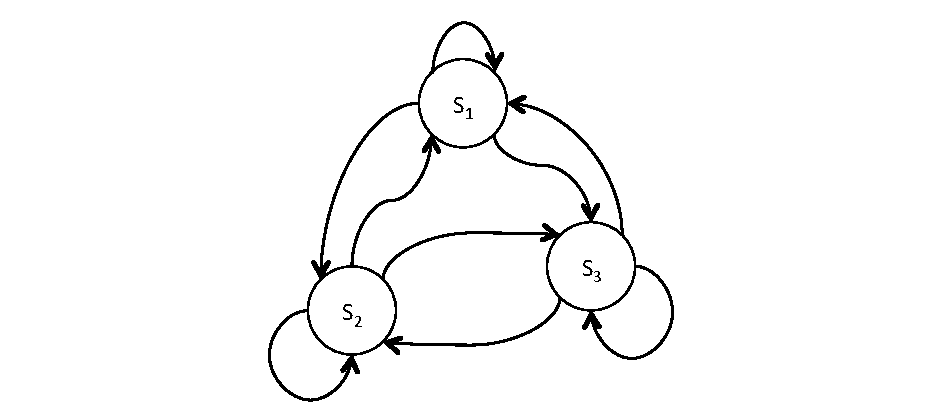
\includegraphics[width=\textwidth]{markov.pdf}
        \caption{State transition process of a Markov chain}
        \label{fig:markov:transition}
        \end{figure}
Illus.\,\ref{fig:markov:transition} visually shows a typical Markov chain.
The state space in this case is finite (three in fact) and 
the process is the transition from the states to one another.

We have given the definition of the state transition matrix 
with Def.\,\ref{defn:markov} in Sec.\,\ref{sec:preliminary:markov:definition}.
For every finite-state time-homogeneous Markov chain, 
we have the following theorem.

		\begin{thm}
		\label{thm:CK}
		For finite-state time-homogeneous Markov chains and any $t,u \in \hn$, we have
			\begin{equation}
			\label{eq:preliminary:markov:CK}
			\bGamma^{(t+u)} = \bGamma^{(t)}\bGamma^{(u)}.
			\end{equation}
		Eq.\,\ref{eq:preliminary:markov:CK} is known as Chapman-Kolmogorov equation.
		\end{thm}
If we denote the $1$-step transition matrix $\bGamma^{(1)}$ as $\bGamma$, 
then we shall deduce the following corollary.
		
		\begin{cor}
		\label{cor:CK}
		For every finite-state time-homogeneous Markov chain and any $t \in \hn$, we have
			\begin{equation}
			\label{eq:preliminary:markov:CK_2}
			\bGamma^{(t)} = \bGamma^t,
			\end{equation}
		that is, the $k$-step transition matrix is entirely decided by the $1$-step transition matrix.
		\end{cor}
Now we give the definition of the initial distribution of a Markov chain,
and we shall find the unconditional distribution of the chain at a given time.

		\begin{defn}
		\label{defn:initial}
		We call the row vector
			\begin{equation}
			\label{eq:preliminary:markov:initial}
			\bdelta(t) = \left(\prob{S_t=1},\dots,\prob{S_t=N}\right)
			\end{equation}
		the unconditional probabilities of a Markov chain at time $t$.
		In particular, we refer to $\bdelta(1) := \bpi$ as the initial distribution of the Markov chain.
		\end{defn}
Then with the definition and Cor.\,\ref{cor:CK}, we have
		\begin{equation}
		\label{eq:preliminary:markov:unconditional}
		\bdelta(t+1) = \bdelta(t)\bGamma = \bpi\bGamma^{t}.
		\end{equation}
The equation implies that the unconditional distribution relies fully on 
the initial distribution and the state transition matrix.


\subsection{Stationary distributions}
\label{sec:preliminary:markov:stationary}
At last we introduce the idea of stationary distribution.

		\begin{defn}
		\label{defn:stationary}
		For a Markov chain, if there exists a row vector $\{v_j \colon j \in \hs\}$ that satisfies
			\begin{subequations}
			\begin{align}
			&v_j  \geq 0, j \in \hs; \\
			&\sum_{j \in \hs} v_j = 1;\\
			&v_j  = \sum_{i \in \hs} v_i\gamma_{ij},
			\end{align}
			\end{subequations}
		then we call $V := \{v_j \colon j \in \hs\}$ the stationary distribution of the Markov chain.
		\end{defn}
The equations above guarantees that $V$ is simutaneously a probability distribution and stationary.

The introduction of stationary distribution is because that 
the state transition matrix will converge.
We state the property as the following theorem.

		\begin{thm}
		\label{thm:stationary}
		For an ergodic finite-space time-homogeneous Markov chain,
		the limit distribution is stationary, i.e.
			\begin{equation}
			\label{eq:preliminary:markov:stationary}
			\lim_{n \ra \infty} \bpi\bGamma^{n} = V.
			\end{equation}
		\end{thm}
One of the results of Thm.\,\ref{thm:stationary} is that forecast result in hidden Markov models
converges with increasing forecast steps
(see Sec.\,\ref{sec:HMM:predeco:forecast}).

%%%%%%%%%%%%%%%%%%%%%%%%%%

\section{K-Means clustering}
\label{sec:preliminary:kmeans}
Data clustering is a popular technique in time series analysis.
It enables us to cluster sub-populations with different properties so that 
more accurate analysis results could be available,
considering the heterogeneity of the sample data.

K-Means, of all existing data clustering techniques,
is the most common and universally acknowledged one.
The name is firstly used in \cite{Macqueen:1967uv}.
The idea originates from signal processing theories, 
which is known as vector quantization (VQ),
and now is prevalent for cluster analysis and data mining.

The standard algorithm for K-Means was proposed by Stuart Lloyd in 1957 and 
by E.\,W.~Forgy in 1965 \cite{Forgy:1965cl} separately, 
which is known as Lloyd-Forgy algorithm.
A more efficient algorithm is proposed by Hartigan in \cite{Hartigan:1975cl}.

Clustering itself has been commonly implemented in financial data analysis
(e.g.\,see \cite{Cont:2001gv,Babu:2012wl,Gupta:2014tp}),
while we introduce the K-Means algorithm merely to find the initial distribution 
of the hidden Markov model (see Sec.\,\ref{sec:system:function:init}),
thus we only provide a very brief introduction here.


\subsection{Model formulation and aims}
\label{sec:preliminary:kmeans:formulation}
Firstly we state the K-Means clustering problem.

Given observation set $\{\bx_1,\bx_2,\dots,\bx_n\}$ where $\bx$ is a $d$-dimensional vector,
we aim to partition the $n$ observations into $k (k\leq n)$ sub-sets $\{S_1,S_2,\dots,S_k\}$
in order to minimize the within-cluster sum of squares (WCSS), 
which is the sum of distance functions of each point in the cluster to the center.
The formulation of this problem is given as follow:
		\begin{equation}
		\label{eq:preliminary:kmeans}
		\min_{\bS} \sum_{i=1}^{k}\sum_{\bx \in S_i} \norm{\bx - \bmu_i}^2,
		\end{equation}
where $\bmu_i$ is the mean of points of $S_i$ (center),
and $\bS$ is the $k$ sub-sets.

The clustering centers found by the K-Means algorithm shall be
appropriate guesses for the initial distribution.


\subsection{The K-Means algorithm}
\label{sec:preliminary:kmeans:algo}
The standard algorithm processes iteratively.

Given a set of initial guess of $k$ means $\{m_1^{(1)},m_2^{(1)},\dots,m_k^{(1)}\}$,
we firstly assign each observation to the cluster whose mean yields the least WCSS,
which is known as the assignment step.
		\begin{equation}
		\label{eq:preliminary:kmeans:assign}
		S_i^{(t)} = \left\{x_p \colon \norm{x_p-m_i^{(t)}}^2 \leq \norm{x_p-m_j^{(t)}}^2,
			\forall j,\ 1\leq j \leq k  \right\}.
		\end{equation}
Each $x_p$ is assigned to one and only one set $S_i$.

Then we calculate the new means to be the centroids of the observations in the new clusters,
which is known as the update step.
		\begin{equation}
		\label{eq:preliminary:kmeans:update}
		m_i^{(t+1)} = \frac{1}{\abs{S_i^{(t)}}} \sum_{x_j \in S_i^{(t)}} x_j.
		\end{equation}
The two steps are performed in sequence until convergence of the result.

Notice that the algorithm only yields a local optimum 
but has no guarantees on finding the global one.
The result is enough for the analysis we will carry out in empirical analysis.
Since the algorithm is not the major concern of this thesis,
the programming realization of K-Means implement 
the \texttt{sklearn.cluster.KMeans} module directly for convenience
(see Appendix \ref{app:code}).



% !TEX encoding = UTF-8 Unicode
%%==================================================
%% thanks.tex for SJTU Bachelor Thesis
%% version: 0.5.2
%% Encoding: UTF-8
%%==================================================

\chapter{Hidden Markov Models}
\label{chap:HMM}

In this chapter we formally introduce the hidden Markov models (HMM).
In Sec.\,\ref{sec:HMM:overview} we examine the structure of HMM and 
some fundamental but significant statistics.
A brief introduction to the history of HMM is also covered.
The core part of this chapter lies in Sec.\,\ref{sec:HMM:EM},
i.e.\,how to estimate the model parameters for further analysis and predictions 
with the so-called Baum-Welch or Expectation Maximization (EM) algorithm.
Principles and derivations are explained in details, 
and every module and step of the algorithm is specified.
Sec.\,\ref{sec:HMM:predeco} firstly introduces the method to forecast the series 
based on model parameters deduced with the algorithm.
Then we discuss about techniques to analyze the behavior of the hidden states,
which is known as decoding.

%%%%%%%%%%%%%%%%%%%%%%%%%%

\section{Model overview}
\label{sec:HMM:overview}
As is apparently indicated in its name, 
a hidden Markov model (HMM) is closely related to Markov chains but
with additional existence of latent elements.
Generally speaking, a HMM is a doubly stochastic process \cite{Rabiner:1986jk}.
One stochastic process cannot be directly observed while
the other sequence is observable,
of which the probability distribution of the observed variable is 
conditional on the hidden states,
i.e.\,the underlying and unobserved process.
Specifically, the underlying process is considered to satisfy the Markovian property
and HMM is thus named.
HMM is also known as `hidden Markov process' \cite{Ephraim:2002ju},
`Markov-dependent mixture' \cite{Leroux:1992ma},
`Markov-switching model' \cite{Haas:2004ek},
`Markov mixture model' or `models subject to Markov regime' \cite{Zucchini:2009df},
and these are just different names of HMM.

The model was firstly proposed by Ruslan L.~Stratonovich in \cite{Stratonovich:1960vh},
who also firstly propose the forward-backward procedure (see Sec.\,\ref{sec:HMM:EM:fwdbwd}).
As we described in Sec.\,\ref{sec:preliminary:markov},
states in a typical Markov chain are observable,
thus the only parameters need estimating are the state transition probabilities (matrix).
In a HMM, one of the two series is visible and 
each output is distributed conditional on the hidden states.
The hidden states are distributed in a potential set with corresponding symbols.
The directly observed sequence and the sequence of state symbols 
(which might need to be deduced from the observations)
together provide information about the model.

HMM, due to its probabilistic property, 
is considered as the simplest form of a dynamic Bayesian network \cite{wiki:hmm}.
Besides its application in the financial industry (see Sec.\,\ref{sec:introduction:background}),
the model is mainly applied to pattern recognition 
such as speech recognition and part-of-speech tagging \cite{wiki:hmm,Rabiner:1989hs},
and bioinfomatics like health trajectory \cite{Ghassempour:2014ew}.

In more general HMMs,
the latent variable is not limited to the form of hidden states represented with tokens.
The latent variables themselves could be mathematically meaningful,
either discrete or continuous.
We will cover this part in Sec.\,\ref{sec:future:PF}.
Currently in this section, we only deal with hidden states that are categorical.


\subsection{Model formulation}
\label{sec:HMM:overview:formulation}

        \begin{figure}[!hbt]
        \center
        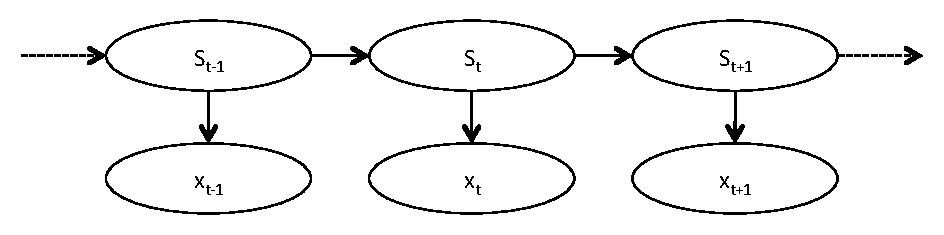
\includegraphics[width=\textwidth]{HMM.pdf}
        \caption{Directed graph of a typical HMM}
        \label{fig:HMM:overview}
        \end{figure}
Illus.\,\ref{fig:HMM:overview} plots a typical HMM in the simplest way.
The model is within the area dependent mixture models,
with $S_t$ representing the hidden states process and 
$X_t$ representing the observed variable,
i.e.\,the visible realizations of the other stochastic process.

The hidden states process $\{S_t \colon t = 1,2,\dots\}$ is a Markov chain: 
        \begin{equation}
        \label{eq:HMM:states}
        \prob{S_t \mid \bS^{(t-1)}} = \prob{S_t \mid S_{t-1}},\ t = 2,3,\dots,
        \end{equation}
and the observed variable has a probability distribution
conditional only on the current hidden state:
        \begin{equation}
        \label{eq:HMM:prob}
        \prob{X_t \mid \bX^{(t-1)}, \bS^{(t-1)}} = \prob{X_t \mid S_t},\ t = 1,2,3,\dots.
        \end{equation}
Values of the hidden states are categorical tokens that qualitatively distinguishes the states.
The number of symbols in the feasible set defines the name of the HMM,
e.g.\,if there are in total $N$ possible hidden states,
the model is then referred to as a $N$-state HMM.
The transition of each state from and to one another 
is exactly the same as one shown in Illus.\,\ref{fig:markov:transition}

The probability $\prob{X_t \mid S_t}$ in Eq.\,\ref{eq:HMM:prob} 
can be used to derive the probability mass/density functions for discrete/continuous observations.
We introduce the notation $p_i$, for $i = 1,2,\dots,N$, where
		\begin{equation}
        \label{eq:HMM:distribution}
        p_i(x) = \left \{ 
        \begin{array}{l l}
        \prob{X_t = x \mid S_t = i} & ,\text{if}\ X_t\ \text{is discrete,} \\
        f_t(x \mid S_t = i) & ,\text{if}\ X_t\ \text{is continuous.} \\
        \end{array} \right.
        \end{equation}
We refer to the $N$ distributions $\{p_i\}_{i=1}^{N}$ as state-dependent distribution, 
or simply conditional distributions, 
since the probability distributions are conditional on the states.
The distributions are irrelevant with time $t$ owing to their time homogeneity.
In the following sections,
we merely consider the case where $X_t$ is discrete,
as the observed stock return series that will be discussed about 
in Ch.\,\ref{chap:system} and \ref{chap:positive} are discretely sampled.


\subsection{Marginal distributions}
\label{sec:HMM:overview:distribution}
With knowledge of Markov chain (Sec.\,\ref{sec:preliminary:markov}) and 
Eq.\,\ref{eq:HMM:states},\ref{eq:HMM:prob} and \ref{eq:HMM:distribution},
we are able to find the marginal distributions of the observed series $X_t$.


Consider the marginal probability
		\begin{equation}
		\label{eq:HMM:marginal}
		\begin{aligned}
		\prob{X_t = x} & = \sum_{i=1}^{N} \prob{X_t = x \mid S_t = i}\prob{S_t = i} \\
		& = \sum_{i=1}^N p_i(x)\delta_i(t).
        \end{aligned}
        \end{equation}
We can rewrite Eq.\,\ref{eq:HMM:marginal} in form of matrix:

		\begin{equation}
		\label{eq:HMM:marginalmat}
		\begin{aligned}
		\prob{X_t = x} & = (\delta_1(t),\delta_2(t),\dots,\delta_N(t)) 
			\left ( \begin{array} {c c c}
				p_1(x) & & 0 \\
				& \ddots & \\
				0 & & p_N(x) \\
			\end{array} \right)
			\left ( \begin{array} {c}
				1 \\	\vdots \\	1 \\
			\end{array} \right) \\
		& = \bdelta(t)\bp(x)\one,
        \end{aligned}
        \end{equation}
where $\bp(x)$ is the diagonalized matrix of $(p_1(t),p_2(t),\dots,p_N(t))$.

Since $\bdelta(t) = \bpi\bGamma^{t-1}$ (Eq.\,\ref{eq:preliminary:markov:unconditional}), 
we shall rewrite Eq.\,\ref{eq:HMM:marginalmat} as 
		\begin{equation}
		\label{eq:HMM:marginalmatsimple}
		\prob{X_t = x} = \bpi\bGamma^{t-1}\bp(x)\one.
        \end{equation}

We also care about the bivariate distribution of $X_t$.
Firstly we consider the joint probability expressed in conditional probabilities:
		\begin{equation}
		\label{eq:HMM:joint}
		\prob{X_t,X_{t+k},S_t,S_{t+k}} = 
			\prob{S_t}\prob{X_t \mid S_t}\prob{S_{t+k} \mid S_t}\prob{X_{t+k} \mid S_{t+k}},
        \end{equation}
which leads to
		\begin{equation}
		\label{eq:HMM:bivariate}
		\begin{aligned}
		\prob{X_t = v,X_{t+k} = w} & = 
			\sum_{i=1}^{N}\sum_{j=1}^{N} \prob{X_t = v,X_{t+k} = w,S_t = i,S_{t+k} = j} \\
		& = \sum_{i=1}^{N}\sum_{j=1}^{N} 
			\prob{S_t = i}p_i(v)\prob{S_{t+k} = j \mid S_t = i}p_j(w) \\
		& = \sum_{i=1}^{N}\sum_{j=1}^{N} \delta_i(t)p_i(v)\gamma_{ij}(k)p_j(w) \\
		& = \bdelta(t)\bp(v)\bGamma^k\bp(w)\one.
        \end{aligned}
        \end{equation}

Thus, we can derive the expectation of $X_t$:
		\begin{equation}
		\label{eq:HMM:expectation}
		E(X_t) = \sum_{i=1}^{N} \delta_i(t)E(X_t \mid S_t = i).
		\end{equation}
Eq.\,\ref{eq:HMM:expectation} plays an important role in 
the series prediction that will be talked about later.

\subsection{The likelihood}
\label{sec:HMM:overview:likelihood}
One of the most important statistics of a statistical model is its (log) likelihood.
Therefore, we present a practical way to compute the likelihood $L_T$
of the $N$-state HMM given observations $\{x_t \colon t = 1,2,\dots,T\}$.
With knowledge of the likelihood,
we shall estimate the model parameters through numerical maximization of the likelihood
or other methods that require computable likelihood.

Consider a $N$-state HMM with initial distribution $\bpi$, 
transition matrix $\bGamma$,
and diagonalized conditional probability density functions $p_i$.
The explicit form of the likelihood is then given by
		\begin{equation}
		\label{eq:HMM:likelihood}
		L_T = \bpi\bp(x_1)\bGamma\bp(x_2)\bGamma\bp(x_3)\cdots\bGamma\bp(x_T)\one.
		\end{equation}
The result is quite elegant and we omit the derivation here,
as it is not the main concern of this work.
The reader shall refer to \cite{Zucchini:2009df} for the proof of this conclusion.
The reader should also notice that \cite{Zucchini:2009df} provides details about the likelihood
when observation data are missing at random or interval-censored.
Corresponding adjustments should be taken to properly calculate the likelihood.
Since the empirical analysis data that we will use in Ch.\,\ref{chap:positive} 
are required to be complete and tidy,
we avoid unnecessary explanations for these cases in this thesis.

%%%%%%%%%%%%%%%%%%%%%%%%%%

\section{Model estimation with Expectation Maximization algorithm}
\label{sec:HMM:EM}
Knowing how to compute the likelihood of a HMM, 
we can estimate the model parameters by direct maximization of the likelihood,
i.e.\,fulfill the task of model estimation with MLEs.
Another commonly implemented method is the so-called Expectation Maximization (EM) algorithm.

The EM algorithm is specifically known as Baum-Welch algorithm within the area of HMMs,
and the method is firstly proposed in \cite{Baum:1966cy,Baum:1967gs,Baum:1970do}.
The algorithm deals with Markovian hidden states series 
that is homogeneous but not necessarily stationary.
Apart from the state transition matrix,
the initial distribution $\bpi$ is also estimated and 
so is the conditional distribution probability density function.
We will first introduce the forward and backward procedure in Sec.\,\ref{sec:HMM:EM:fwdbwd}
and then present the full version of EM in Sec.\,\ref{sec:HMM:EM:algo}.


\subsection{Forward and backward procedure}
\label{sec:HMM:EM:fwdbwd}
Recall Eq.\,\ref{eq:HMM:likelihood} for the form of likelihood:
		\begin{equation*}
		\label{eq:HMM:likelihood2}
		L_T = \bpi\bp(x_1)\bGamma\bp(x_2)\bGamma\bp(x_3)\cdots\bGamma\bp(x_T)\one,
		\end{equation*}
and we provide the definitions of forward and backward probabilities as follows.
		
		\begin{defn}
		\label{defn:fwd}
		For $t = 1,2,\dots,T$, define the row vector $\balpha_t$ as
			\begin{equation}
			\label{eq:HMM:fwd:defn}
			\balpha_t = \bpi\bp(x_1)\bGamma\bp(x_2)\bGamma\bp(x_3)\cdots\bGamma\bp(x_t)
			 = \bpi\bp(x_1)\prod_{s=2}^{t}\bGamma\bp(x_s),
			\end{equation}
		and refer to the elements as forward probabilities.
		\end{defn}

		\begin{defn}
		\label{defn:bwd}
		For $t = 1,2,\dots,T$, define the row vector $\bbeta_t$ as
			\begin{equation}
			\label{eq:HMM:bwd:defn}
			\bbeta_t = \bGamma\bp(x_{t+1})\bGamma\bp(x_{t+2})\cdots\bGamma\bp(x_T)\one
			 = \left(\prod_{s=t+1}^{T}\bGamma\bp(x_s)\right)\one,
			\end{equation}
		and refer to the elements as backward probabilities. 
		The case $t = T$ yields $\bbeta_T = 1$.
		\end{defn}

It is easy to find that we can rewrite Eq.\,\ref{eq:HMM:fwd:defn} in the form of recursion that 
for $t = 1,2,\dots,T-1, \balpha_{t+1} = \balpha_t\bGamma\bp(x_{t+1})$.
With derivation based on Bayesian formula 
(similar to \ref{eq:HMM:likelihood},see \cite{Zucchini:2009df}),
we have the following proposition:

		\begin{prop}
		\label{prop:fwd}
		For $t = 1,2,\dots,T$ and $j = 1,2,\dots,N$,
			\begin{equation}
			\label{eq:HMM:fwd:prop}
			\alpha_t(j) = \prob{\bX^{(t)} = \bx^{(t)}, S_t = j}.
			\end{equation}
		The element $\alpha_t(j)$ is thus called the forward probability.
		\end{prop}

Similarly, we can rewrite Eq.\,\ref{eq:HMM:bwd:defn} as that 
for $t = 1,2,\dots,T-1, \bbeta_{t}^{\prime} = \bGamma\bp(x_{t+1})\bbeta_{t+1}^{\prime}$,
and suggest the similar proposition:
	
		\begin{prop}
		\label{prop:bwd}
		For $t = 1,2,\dots,T-1$ and $i = 1,2,\dots,N$,
			\begin{equation}
			\label{eq:HMM:bwd:prop}
			\beta_t(i) = \prob{\bX^{(t+1:T)} = \bx^{(t+1:T)} \mid S_t = i},\ \prob{S_t = i}>0.
			\end{equation}
		The element $\beta_t(i)$ is thus called the backward probability.
		\end{prop}
Note that the forward probabilities are joint probabilities while
backward probabilities are conditional probabilities.

With Eq.\,\ref{eq:HMM:likelihood},\ref{eq:HMM:fwd:prop} and \ref{eq:HMM:bwd:prop},
we can rewrite the likelihood with forward and backward probabilities:
		\begin{equation}
		\label{eq:HMM:likelihood:fwdbwd}
		\alpha_t(i)\beta_t(i) = \prob{\bX^{(T)} = \bx^{(T)}, S_t = i} \LRa
		L_T = \prob{\bX^{(T)} = \bx^{(T)}} = \balpha_t\bbeta_t^{\prime}.
		\end{equation}
The equation can be easily proved with Def.\,\ref{defn:fwd} and \ref{defn:bwd} 
and we omit the derivation here.

In order to apply the results to the EM algorithm,
we also need the conditional probabilities of the hidden states given observations.
	
		\begin{prop}
		\label{prop:states}
		For $t = 1,2,\dots,T$,
			\begin{equation}
			\label{eq:HMM:states:cond}
			\prob{S_t = j \mid \bX^{(T)} = \bx^{(T)}} = \frac{\alpha_t(j)\beta_t(j)}{L_T},
			\end{equation}
		and for $t = 2,\dots,T$,
			\begin{equation}
			\label{eq:HMM:states:trans}
			\prob{S_{t-1} = j,S_t = k \mid \bX^{(T)} = \bx^{(T)}} = 
			\frac{\alpha_{t-1}(j)\gamma_{jk}p_k(x_t)\beta_t(k)}{L_T},
			\end{equation}
		\end{prop}
Results in Prop.\,\ref{prop:states} will be applied in both model estimation and decoding.


\subsection{The EM algorithm}
\label{sec:HMM:EM:algo}
The traditional EM algorithm iteratively maximize the likelihood of the model
and to find the MLEs under circumstances of missing data.
Baum-Welch algorithm refers to this idea and consider the sequence of hidden states
as missing data since they are unobserved.

We denote the model parameters as $\btheta$ and try to compute the 
complete-data log-likelihood (CDLL),
i.e.\,the log-likelihood of parameters $\btheta$.
Then EM can be carried out by two steps:
		\begin{itemize}
		\item \textbf{E step} calculates the expectations of (functions of) the missing data 
		conditional on the observations and the current estimate of $\btheta$.
		\item \textbf{M step} maximizes the CDLL w.r.t.\,$\btheta$.
		\end{itemize}
The iteration carries on until convergence,
and the final $\btheta$ is the stationary point of the likelihood,
which is the model parameter set that we want to figure out.

We define two indicators, of which the value is either zero or one.
		\begin{equation}
		\label{eq:HMM:EM:indicator}
		u_j(t) = \left \{ \begin{array}{l l}
		1 & ,\text{iff}\ S_t = j \\
		0 & ,\text{otherwise}, \\
		\end{array} \right.
		\text{and}\quad
		v_{jk}(t) = \left \{ \begin{array}{l l}
		1 & ,\text{iff}\ S_{t-1} = j\ \text{and}\ S_t = k \\
		0 & ,\text{otherwise}. \\
		\end{array} \right.
		\end{equation}
Then we rewrite the likelihood of HMM,
viewing hidden states $S_1,S_2,\dots,S_T$ as missing data,
in terms of the indicators and parameters:
		\begin{equation}
		\label{eq:HMM:EM:CDLL}
		\log\left(\prob{\bx^{(T)},\bs^{(T)}}\right) = 
		\underbrace{\sum_{j=1}^{N} u_j(1)\log\pi_j}_{\text{term 1}} + 
		\underbrace{\sum_{j=1}^{N}\sum_{k=1}^{N} \left(\sum_{t=2}^Tv_{jk}(t)\right)\log\gamma_{jk}}
			_{\text{term 2}} + 
		\underbrace{\sum_{j=1}^{N}\sum_{t=1}^{T} u_j(t)\log p_j(x_t)}_{\text{term 3}}.
        \end{equation}
Iterative maximization of the CDLL will provide us information about 
both $\bpi$, the initial distribution and $\bGamma$, the state transition matrix.

Apply Eq.\,\ref{eq:HMM:EM:CDLL} to the general EM and we can specify the two steps as
		\begin{itemize}
		\item \textbf{E step} replaces the two indicator vectors by their conditional expectations
		given observations $\bx^{(T)}$ and the current parameter estimates
			\begin{subequations}
			\begin{align}
			\label{eq:HMM:EM:ind_u}
			\hat{u}_j(t) & = \prob{S_t = j \mid \bx^{(T)}} = \frac{\alpha_t(j)\beta_t(j)}{L_T},\\
			\label{eq:HMM:EM:ind_v}
			\hat{v}_{jk}(t) & = \prob{S_{t-1} = j,S_t = k \mid \bx^{(T)}} = 
				\frac{\alpha_{t-1}(j)\gamma_{jk}p_k(x_t)\beta_t(k)}{L_T}.
			\end{align}
			\end{subequations}
		\item \textbf{M step} maximizes the CDLL, Eq.\,\ref{eq:HMM:EM:CDLL},
		w.r.t.\,the initial distribution $\bpi$, the state transition matrix $\bGamma$,
		and conditional distribution parameters which is embedded in $p_j(x_t)$ in term 3.
		\end{itemize}

Notice that we have split the computation of CDLL into three terms 
so that the maximizations w.r.t.\,the three parameter sets are independent.
Furthermore, the separation guarantees the existence of analytic solutions.
We present the sub-problems and corresponding solutions as follows.

\subsubsection{Initial distribution}
\label{sec:HMM:EM:algo:initial}
By term 1 in Eq.\,\ref{eq:HMM:EM:CDLL}, consider the maximization problem
		\begin{equation}
		\label{eq:HMM:EM:max:1}
		\max_{\bpi} \sum_{j=1}^{N} u_j(1)\log\pi_j,
		\end{equation}
and the solution is given as
		\begin{equation}
		\label{eq:HMM:EM:sol:1}
		\pi_j = \frac{\hat{u}_j(1)}{\sum_{j=1}^{N}\hat{u}_j(1)} = \hat{u}_j(1).
		\end{equation}


\subsubsection{State transition matrix}
\label{sec:HMM:EM:algo:transition}
By term 2 in Eq.\,\ref{eq:HMM:EM:CDLL}, consider the maximization problem
		\begin{equation}
		\label{eq:HMM:EM:max:2}
		\max_{\bGamma} \sum_{j=1}^{N}\sum_{k=1}^{N} \left(\sum_{t=2}^Tv_{jk}(t)\right)\log\gamma_{jk},
		\end{equation}
and the solution is given as
		\begin{equation}
		\label{eq:HMM:EM:sol:2}
		\begin{aligned}
		\gamma_{jk} & = \frac{f_{jk}}{\sum_{k=1}^{N} f_{jk}}, \\
		\text{where}\quad f_{jk} & = \sum_{t=2}^{T} \hat{v}_{jk}(t).
		\end{aligned}
		\end{equation}


\subsubsection{Conditional distribution}
\label{sec:HMM:EM:algo:distribution}
By term 3 in Eq.\,\ref{eq:HMM:EM:CDLL}, consider the maximization problem
		\begin{equation}
		\label{eq:HMM:EM:max:3}
		\max_{\btheta} \sum_{j=1}^{N}\sum_{t=1}^{T} u_j(t)\log p_j(x_t;\btheta).
		\end{equation}
The solution to this sub-problem depends on the formulation of the conditional distribution,
and is deduced through common MLE method.
We provide solutions to two kind of distributions here,
one for Poisson and the other for normal.

For Poisson distributions we have $p_j(x) = e^{-\lambda_j}\frac{\lambda_j^x}{x!}$,
the solution is then given as 
		\begin{equation}
		\label{eq:HMM:EM:sol:3:poisson}
		\hat{\lambda}_j = \frac{\sum_{t=1}^{T} \hat{u}_j(t)x_t}{\sum_{t=1}^{T} \hat{u}_j(t)}.
		\end{equation}

For normal distributions we have 
$p_j(x) = \frac{1}{\sqrt{2\pi\sigma_j^2}} \exp\{-\frac{(x-\mu_j)^2}{2\sigma_j^2}\}$,
the solution is then given as 
		\begin{subequations}
		\begin{align}
		\label{eq:HMM:EM:sol:3:normal:mu}
		\hat{\mu}_j & = \frac{\sum_{t=1}^{T} \hat{u}_j(t)x_t}{\sum_{t=1}^{T} \hat{u}_j(t)}, \\
		\label{eq:HMM:EM:sol:3:normal:sigma}
		\hat{\sigma}_j & = \frac{\sum_{t=1}^{T} \hat{u}_j(t)(x_t - \hat{\mu}_j)^2}
							  {\sum_{t=1}^{T} \hat{u}_j(t)}.
		\end{align}
		\end{subequations}
The results above are thus easy to compute and can be 
directly applied in the numerical realization procedures.

%%%%%%%%%%%%%%%%%%%%%%%%%%

\section{Prediction and decoding}
\label{sec:HMM:predeco}
The series prediction is essentially an application of the forecast distributions.
With model parameters estimated,
we can fulfill the prediction by one-step or multiple-step forecast.
We cover this topic in Sec.\,\ref{sec:HMM:predeco:forecast}.

Information of the historical hidden states distributions can be also deduced.
The process of find the states occupied by the Markov chain is referred to as decoding,
Decoding can be further classified as local ones and global ones
in terms of the likelihood to be maximized.
Both decoding procedures are discussed in this section.
Specifically, we introduce the Viterbi algorithm that is implemented for global decoding 
in Sec.\,\ref{sec:HMM:predeco:glodeco}.


\subsection{Forecast distributions}
\label{sec:HMM:predeco:forecast}
Consider $h$-step forecast distribution conditional on the observations
		\begin{equation}
		\label{eq:HMM:predeco:forecast}
		\begin{aligned}
		\prob{X_{T+h} = x \mid \bX^{(T)} = \bx^{(T)}} & = 
			\frac{\prob{\bX^{(T)} = \bx^{(T)}, X_{T+h} = x}}{\prob{\bX^{(T)} = \bx^{(T)}}} \\
		& = \frac{\balpha_T\bGamma^h\bp(x)\one}{\balpha_T\one}. 
		\end{aligned}
		\end{equation}
In order to perform one-step prediction,
we can simply assign $h$ with value one and obtain the result.

Notice that when $h$ increases, 
the result stated in Eq.\,\ref{eq:HMM:predeco:forecast} will converge
due to the convergence of Markov chain state transition matrix, i.e.
		\begin{equation}
		\label{eq:HMM:predeco:forecast:converge}
		\lim_{h\ra\infty}\prob{X_{T+h} = x \mid \bX^{(T)} = \bx^{(T)}} = \bdelta^{\ast}\bp(x)\one,
		\end{equation}
where $\bdelta^{\ast}$ represents the stationary distribution of the Markov chain
(see Sec.\,\ref{sec:preliminary:markov:stationary}).
One of the direct influences of the convergence is that
we cannot take a too big $h$ in our stock return series prediction system,
or the prediction results would be smoothed due to the converging property.


\subsection{State probabilities and local decoding}
\label{sec:HMM:predeco:locdeco}
The concept of decoding is firstly adopted in speech recognition areas \cite{Fredkin:1992ba},
and, in the context of HMM,
refers to the procedure to find the most probable sequence of hidden states
that generates the observation series.
The idea `local decoding' of the state at a specific time 
stands for the determination of the most possible state at that time node.

Recall Eq.\,\ref{eq:HMM:states:cond}
		\begin{equation*}
		\prob{S_t = j \mid \bX^{(T)} = \bx^{(T)}} = \frac{\alpha_t(j)\beta_t(j)}{L_T},
		\end{equation*}
we are able to compute the likelihood $L_T$ with EM algorithm,
and therefore able to calculate the state probabilities and 
decide the most probable state at each $t$:
		\begin{equation}
		\label{eq:HMM:predeco:locdeco:state}
		S_t^{\ast} = \argmax_{j = 1,2,\dots,N} \prob{S_t = j \mid \bX^{(T)} = \bx^{(T)}}.
		\end{equation}


\subsection{Global decoding and Viterbi algorithm}
\label{sec:HMM:predeco:glodeco}
Local decoding only provides information of the most probable state for each separate time $t$
but tells nothing about the most likely sequence of the states over the entire period.
Global decoding solves a slightly different maximization problem as local decoding,
and the result is often similar but not exactly identical.

The global decoding procedure enables us to find 
the conditional probability of the entire hidden state series given the observations, i.e.
		\begin{equation}
		\label{eq:HMM:predeco:glodeco:prob}
		\prob{\bS^{(T)} = \bs^{(T)} \mid \bX^{(T)} = \bx^{(T)}}.
		\end{equation}

The maximization problem can be solved with an algorithm named after Viterbi \cite{Viterbi:1967hq},
which is a very effective dynamic programming technique.
Define the probabilities $\xi_{ti}$ as follows:
		\begin{equation}
		\label{eq:HMM:predeco:viterbi:defn}
		\begin{aligned}
		\xi_{1i} & = \prob{S_1 = i,X_1 = x_1} = \pi_ip_i(x_1), \\
		\xi_{ti} & = \max_{s_1,s_2,\dots,s_{t-1}} 
			\prob{\bS^{(t-1)} = \bs^{(t-1)},S_t = i, \bX^{(T)} = \bx^{(T)}},
		\end{aligned}
		\end{equation}
for $t = 2,3,\dots,T$.
We can also rewrite Eq.\,\ref{eq:HMM:predeco:viterbi:defn} in a recursive form:
		\begin{equation}
		\label{eq:HMM:predeco:viterbi:defn_2}
		\begin{aligned}
		\xi_{1i} & = \prob{S_1 = i,X_1 = x_1} = \pi_ip_i(x_1), \\
		\xi_{tj} & = \left(\max_i(\xi_{t-1,i}\gamma_{ij})\right)p_j(x_t),
		\end{aligned}
		\end{equation}
for $t = 2,3,\dots,T$ and $i = 1,2,\dots,N$.
The $T\times N$ matrix enables us to solve the maximization problem with 
computational complexity that is linear in $T$.
The result can be solved recursively from:
		\begin{equation}
		\label{eq:HMM:predeco:viterbi:defn_3}
		\begin{aligned}
		S_T & = \argmax_{i = 1,2,\dots,N} \xi_{Ti}, \\
		S_t & = \argmax_{i = 1,2,\dots,N} (\xi_{ti}\gamma_{i,S_{t+1}}),
		\end{aligned}
		\end{equation}
for $t = T-1, T-2,\dots,1$.

The maximization can also be rewritten in form of logarithms,
and scaling problems should be noticed to avoid numerical underflows.
This problem is explained in \cite{Zucchini:2009df} with details.





% !TEX encoding = UTF-8 Unicode
%%==================================================
%% thanks.tex for SJTU Bachelor Thesis
%% version: 0.5.2
%% Encoding: UTF-8
%%==================================================

\chapter{Stock Return Series Prediction System}
\label{chap:system}

This chapter explains in details about the composition of 
the stock return series prediction system and functionality of each module.
Sec.\,\ref{sec:system:overview} firstly present an overview of the system,
introducing the entire data flow and module connection.
Then, in Sec.\,\ref{sec:system:function}, structure of each part is analyzed,
including its intention, input and output, and settings specific to this thesis.
Sec.\,\ref{sec:system:improvement} focuses on some of these settings 
and proposes several ideas concerning potential for improvement.
The full version of the system realization with Python programming is appended to the thesis 
in Appendix \ref{app:code}.

%%%%%%%%%%%%%%%%%%%%%%%%%%

\section{Overview}
\label{sec:system:overview}

		\begin{figure}[!hbt]
        \center
        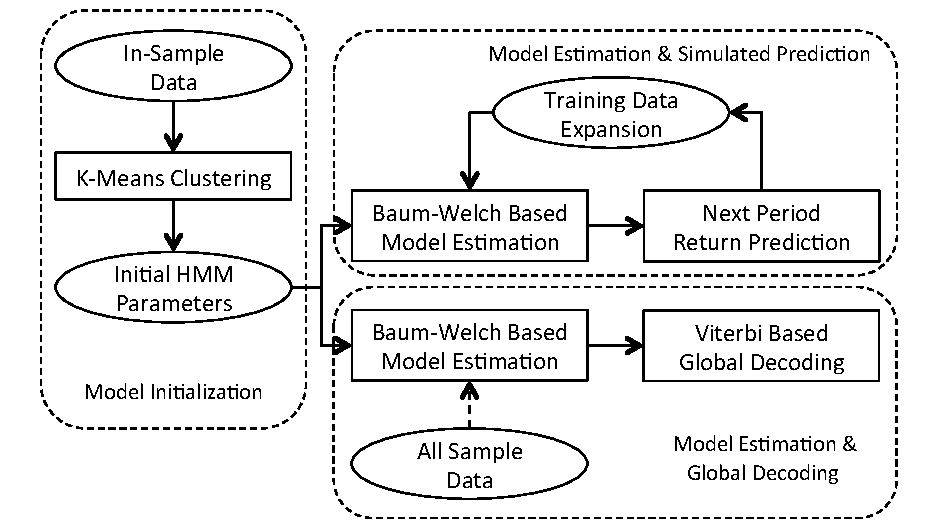
\includegraphics[width=\textwidth]{system.pdf}
        \caption{Overview of the stock return series prediction system}
        \label{fig:system:overview}
        \end{figure}
The stock return series prediction system is composed of two major parts,
model initialization, and simulated prediction; 
the latter part can be further split into two sub-parts, 
model estimation with Baum-Welch (EM) algorithm and prediction based on the model.
Apart from these two major parts, 
a global decoding module is also included in the system 
with purpose to conducted analysis of sample data within the entire observation period.

Illus.\,\ref{fig:system:overview} is a brief overview of the system.
The organization of the system are constructed and will be explained accordingly as follows
	\begin{itemize}
	\item \textbf{Model initialization,} including data pre-processing,
		  initial guesses for parameters based on K-Means clustering.
	\item \textbf{Simulated prediction,} including two sub-parts:
		  \begin{enumerate}
		  \item \textbf{EM based model estimation,} i.e.\,estimation of the state transition matrix
		  		and conditional distribution parameters with EM algorithm.
		  \item \textbf{Prediction,} for stock return of the next period based on 
		  		aforementioned model estimation results.
		  \end{enumerate}
	\item \textbf{Global decoding,} including model estimation and 
		  decoding based on Viterbi algorithm. 
		  The model in this part takes in all sample data in order to 
		  provide analysis of the entire period and the most likely sequence of hidden states.
	\item \textbf{Results saving and visualization.} This part is significant to the system in practice,
		  but needless to be explained in details. 
		  All numerical results are exported in the form of \texttt{.csv} files and 
		  visualizations are carried out on the results.
	\end{itemize}

%%%%%%%%%%%%%%%%%%%%%%%%%%

\section{System composition and functionality}
\label{sec:system:function}
This section is focused on detailed descriptions of 
each part listed above in Sed. \ref{sec:system:overview}.
The part of results saving and visualization is, however, omitted in this section
since the process is more about convenience and intuition 
while it has very little to do with the system itself.


\subsection{Model initialization}
\label{sec:system:function:init}
The data pre-processing work include data downloading and tidying.
A complete input data file consists of two columns, 
the first standing for the timeline and the second for the observed closing prices.
Timeline should be uniformed for each trading day (or trading year in daily cases),
and thus missing value of closing prices should be filled.
Here we fill the missing ones with previous values,
but it is not the only method and sometimes 
linear interpolation or even spline interpolation are implemented for data filling
(e.g.\,see \cite{Beckers:2003do,Reuter:2007cv}).

In order to construct a K-Means model, 
further adjustment and transformation should be made on the raw data.
Firstly we calculate the log return series out of the price series,
and then estimate the standard deviation on each observing time node
through calculating the rolling historical standard errors,
as is shown in Eq.\,\ref{eq:system:data}
		\begin{equation}
		\label{eq:system:data}
		\begin{aligned}
		\text{log return}: r_t & = ln\big( \frac{P_{t}}{P_{t-1}} \big),\ t = 1,2,\dots, \\
		\text{standard deviation}: \sigma_t & = 
			\sqrt{\frac{1}{nf - 1}\sum_{i=t-nf+1}^{nf} (r_i - \bar{r})^2},\ t \geq nf.
		\end{aligned}
		\end{equation}
where $n$ is the number of rolling days and $f$ represents the number of data within each trading day.
For data with different observation frequency, 
$f$ vary (e.g.\,$f=1$ for daily data and $f=24$ for 10min data) but we keep $n$ the same;
more specifically, we choose $n=5$ in this system.

		\begin{figure}[!hbt]
        \center
        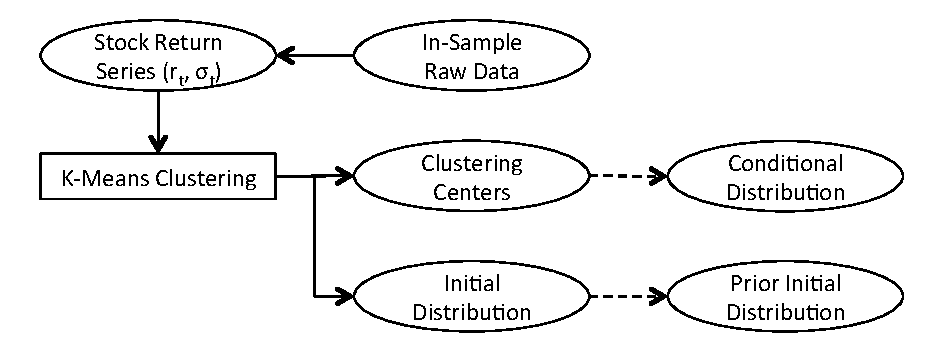
\includegraphics[width=\textwidth]{initialization.pdf}
        \caption{Model initialization module}
        \label{fig:system:init}
        \end{figure}
Now K-Means model takes in a two dimensional time series,
i.e.\,the stock return series and 5-day historical standard deviation series.
Given the number of states, $k$, 
the model generates $k$ clustering centers and corresponding probability distribution,
which are then taken as initial guesses for HMM conditional distribution parameters 
and initial state distribution separately.
Initial guesses for each entry of the transition matrix is arbitrarily set as equal.
The process follows the steps in Illus.\,\ref{fig:system:init}

Notice that K-Means is a very common method to 
find the prior distribution of the parameters \cite{Brailovskiy:2014wu},
while there are also some other methods to find the prior,
e.g.\,generating random vector satisfying the numerical constraints \cite{Hassan:2005uw},
or introduction of machine learning techniques like artificial neural networks (ANN) 
and genetic algorithms (GA) \cite{Hassan:2007hk}. 


\subsection{Simulated prediction}
\label{sec:system:function:prediction}
Simulated prediction module processes with a time loop, 
containing two parts within each loop, model estimation and prediction.
Every time a loop is finished,
we incorporate the real historical return of the next period into the training data set
and process the time horizon to the next period,
estimate the model with the new data set in order to 
predict the return of one more next period.
The iterations is visually described in Illus.\,\ref{fig:system:overview}.


\subsubsection{EM based model estimation}
\label{sec:system:function:prediction:EM}

		\begin{figure}[!hbt]
	    \center
	    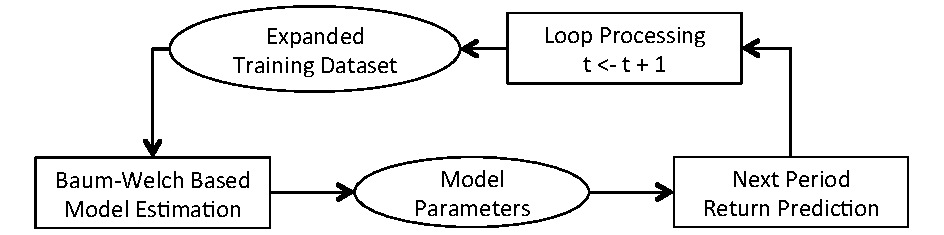
\includegraphics[width=\textwidth]{EM.pdf}
	    \caption{EM based model estimation procedure}
	    \label{fig:system:EM}
	    \end{figure}
Model estimation refers to find the estimations of model parameters, 
including state transition matrix parameters (each entry of the matrix) and
conditional distribution parameters 
(probability density distributions of observed variables conditional on each state).
The method is fully explained in Sec.\,\ref{sec:HMM:EM} 
so we avoid the unnecessary repetition here.
Visual description of the procedure is shown in Illus.\,\ref{fig:system:EM}.

There is something though should be cleared.
As we mentioned before, 
initial guesses for model parameters of the very first loop is found 
with K-Means clustering based on in-sample data.
We use the same initial guesses for all of the following loops,
i.e.\,initialization is carried out only once and 
we no more perform K-Means on the expanded training dataset.
Besides, using the same initial guesses also means that 
the EM algorithm starts from the same parameters for different iterations.
Another way to improve the initial guesses is to 
use the estimation results from the previous loop as the initial guess for the next one,
which shall largely relieve the computational burden and reduce the running time of the system.
However, the change of the training dataset is so small that 
it is reasonable to assume that model parameters change very little.
Thus, it is possible that the initial guess is close enough to the final result 
so that the algorithm prematures due to precision limits,
and that is why the system does not take this way to set the initial guesses.


\subsubsection{Prediction}
\label{sec:system:function:prediction:prediction}
Prediction for the next return is calculated through the estimation results found with EM.
The calculation is simply put as follows:
		\begin{subequations}
		\begin{align}
		\label{eq:system:prediction:ret}
		r_{t+1} & = \bdelta^{\prime} \bGamma \bmu, \\
		\label{eq:system:prediction:std}
		\sigma_{t+1} & = \sqrt{\bdelta^{\prime} \bGamma \bsigma^2},
		\end{align}
		\end{subequations}
where
		\begin{equation}
		\label{eq:system:mu}
		\bmu = (\mu_1, \mu_2, \dots, \mu_N)
		\end{equation}
are expectations of the conditional distributions, and
		\begin{equation}
		\label{eq:system:sigma}
		\bsigma^2 = (\sigma^2_1, \sigma^2_2, \dots, \sigma^2_N)
		\end{equation}
are variances of the conditional distributions,
and $\bdelta$ represents the final distribution of the hidden state 
and $\bGamma$ stands for the state transition matrix.
Notice that an implied assumption of Eq.\,\ref{eq:system:prediction:std} is that
the distributions conditional on hidden states are independent
so the variances are added without covariance terms.
The prediction results are then to be compared with the actual historical returns 
and corresponding standard deviations are used to find the confidence band.

There are two ways to plot the prediction results.
The first one is to fix the price level at the last in-sample date,
of which the stock price is denoted as $P_0$.
We denote the predicted returns as $\hat{r}_i, i = 1,2,\dots,t$,
and thus the prediction result of $\hat{P}_t$ is that
		\begin{equation}
		\hat{P}_t = P_0 e^{\sum_{i=1}^{t}\hat{r}_i}.
		\end{equation}
The second one is called the adaptive prediction, 
which incorporates not only the information of returns but also prices of the data.
In order to predict the price at time $t$, 
we firstly predict the return $\hat{r}_t$ and compute the price given the price at time $t-1$,
that is
		\begin{equation}
		\hat{P}_t = P_{t-1} e^{\hat{r}_t}.
		\end{equation}
In the first kind of prediction, errors of return series predictions accumulate,
so it is very likely that the adaptive prediction performs much better.
We will examine this idea in Ch.\,\ref{chap:positive}.


\subsection{Global decoding}
\label{sec:system:function:decoding}

		\begin{figure}[!hbt]
        \center
        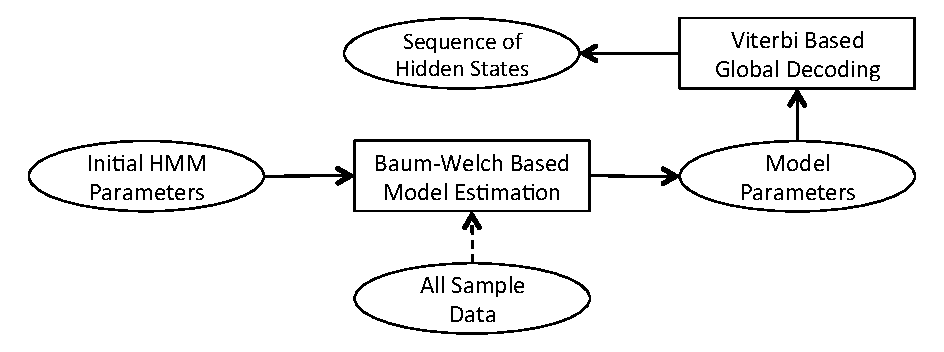
\includegraphics[width=\textwidth]{decoding.pdf}
        \caption{Global decoding module}
        \label{fig:system:decoding}
        \end{figure}
The global decoding module is independent with the simulated prediction module,
and is not the major focus of the prediction system.
The aim of this module is to provide a HMM-based description of 
sample data over the entire observation period.
Traditional methods enable us to know elementary statistics about the data 
(e.g.\,mean, variance, skewness, etc.),
but with Viterbi algorithm we are able to know 
how the hidden states are distributed across the history and 
whether the result matches our conjectures and common senses.

The procedure is illustrated in Illus.\,\ref{fig:system:decoding}.
With initial HMM parameters found in the model initialization module 
(Sec.\,\ref{sec:system:function:init})
we set up the model with all sample data
\footnote{Initial parameters are found with in-sample data instead of all of them. 
Considering the length of out-of-sample data is much shorter than the in-sample,
and the fact that initial guesses do not have large effect on the eventual optimal results,
we choose to remain the initial guesses rather than 
perform another initialization based on all sample data}.
The Viterbi algorithm based decoding is then conducted to 
deduce the most probable sequence of hidden states during the observation period.

%%%%%%%%%%%%%%%%%%%%%%%%%%

\section{Potential for improvement}
\label{sec:system:improvement}
Heretofore the system is complete to perform analysis and predictions 
for the stock return series.
Well functioning as the system is,
it can be further improved and perfected for better performances,
e.g.\,more thorough description of the dataset and more correct and accurate predictions.
We propose several perspectives where potential for improvement may exist.

\subsection{Multiple observed variables}
\label{sec:system:improvement:variable}
Currently the input for the system is a simple observation series on only one variable,
i.e.\,the log return of the stock, derived from its closing price.
However, the information embedded in the single closing price series is so little 
that it cannot capture many of the properties of the stock.
One way to improve the case is to incorporating more observed variables,
e.g.\,opening, low, high and closing prices, 
and to find the conditional observing probability with Gaussian mixture models (GMM)
\cite{Hassan:2005uw,Gupta:2012gm,Brailovskiy:2014wu}.
One of the formulations from \cite{Gupta:2012gm} can be generalized as follows:
		\begin{subequations}
		\begin{align}
		\bo_t & = \big( \frac{\text{close} - \text{open}}{\text{open}},
					  \frac{\text{high} - \text{open}}{\text{open}},
					  \frac{\text{open} - \text{low}}{\text{open}} \big) \\
		b_j(\bo_t) & = \sum_{n = 1}^{N} c_{jn} N(\bo_t,\bmu_{jn},\bsigma_{jn}),
		\end{align}
		\end{subequations}
where $\bo_t$ is the vector of observed variables (observed vector),
$b$ is the observing probability of $\bo_{t}$ conditional on the $j^{th}$ state,
$c$ is the GMM weight and $\bmu, \bsigma$ are GMM parameters.

The idea could be furthered to incorporate more factors apart from the observing prices,
such as financial indicators or economic indicators.
For example, \cite{Wasson:2009dh} presents a way to include Boltzman chain, 
a generalized HMM, into the multi-factor binding genome model.
Including more observed variable may require some other statistical techniques 
since the Gaussian distribution assumption could fail for these variables.
Principal component analysis (PCA) and machine learning theories like neural network (NN)
are commonly implemented methods \cite{Bengio:1992ke,Tipping:1999db,Hassan:2007hk}.


\subsection{Multiseries HMM}
\label{sec:system:improvement:series}
In order to include multiple observed variables, 
the conditional distributions should be accordingly designed and modified.
Another way to make multiple observed variables compact with the original Gaussian distribution
is to introduce the multiseries HMM model,
where the observation is a series of vectors rather than one-dimensional time series.
See \cite{Zucchini:2009df} for more details.


\subsection{Multiple latent variables}
\label{sec:system:improvement:latent}
Apart from improvements from the angle of observed variables,
the latent variable, i.e.\,the hidden states, can also be improved.

The latent variable we use in this thesis is categorical,
which means it merely represents the set of hidden states,
while the states are just labels without realistic statistical meanings.
However, the hidden states can be expressed in other ways that 
they are mathematically meaningful,
and so the latent variable is included in the conditional distribution function of 
the observed variables as a parameter, either discrete or continuous.

For example, time-variation properties are considered for 
the discrete latent variables in \cite{Dias:2015ky};
properties and theories related to continuous latent variables 
are introduced in \cite{Creal:2012ct}.
We will further discuss about the topic in Sec.\,\ref{sec:future:PF}.

Like observed variables, the number of latent variables can be over one
so can the dimension of it, 
and we do not expand the topic here.



% !TEX encoding = UTF-8 Unicode
%%==================================================
%% thanks.tex for SJTU Bachelor Thesis
%% version: 0.5.2
%% Encoding: UTF-8
%%==================================================

\chapter{Empirical Analysis on Stock Market Indices}
\label{chap:positive}

In this chapter we present the numerical results of HMM application for real-world data. 
empirical analysis is conducted on both Chinese and U.S. stock market indices.
We first make several base assumptions on the model and realizations, 
and propose some conjectures on the results, 
including model effectiveness, prediction correctness, 
and possible differences caused by diverse data frequency and observation time period, etc.
We then perform empirical analysis on Standard \& Poor's 500 Index (S\&P 500) and present both 
numerical and visual results in Sec.\,\ref{sec:positive:SP}.
Similar analysis is also carried out on Chinese CSI 300 Index in Sec.\,\ref{sec:positive:CSI}.
We take a further look at the Chinese market and apply the model for data with higher frequencies.
An overall analysis is presented in Sec.\,\ref{sec:positive:result} 
along with comparisons among different data groups.

%%%%%%%%%%%%%%%%%%%%%%%%%%

\section{Assumptions and conjectures}
\label{sec:positive:aspconj}
In this section we specify some basic but necessary assumptions 
for the model application and empirical analysis,
and also propose some conjectures on the prediction result,
including differences in behaviors, potential causes of prediction errors, etc.


\subsection{Assumptions}
\label{sec:positive:aspconj:asp}
The main parameters of a hidden Markov model include 
the state transition matrix and conditional distribution density functions, 
of which dimensions are predetermined by the number of hidden states 
and values are computed through model estimation procedure.

        \begin{asp}
        \label{asp:states}
        The U.S. and Chinese market both have and only have three hidden states,
        namely bear, intermediate and bull.
        \end{asp}
This assumption is intuitively easy to explain.
Usually we tend to describe the market as a bull if the index keeps rising 
and a bear if it goes down all the time.
Sometimes the trend of the index is not that obvious,
daily returns dangle around zero and market volatility is low,
this is when we consider the market as in an intermediate state.
Assuming the market have exactly three states suits customs and has realistic economic meanings.

However, taking the number of states as three might not be statistically optimal,
and we will talk about it in Sec.\,\ref{sec:positive:result:states}.

        \begin{asp}
        \label{asp:distribution}
        Stock returns conditional on the market state are normally distributed.
        Distribution parameters (expectation $\mu$ and variance $\sigma^2$) 
        vary across hidden states and time.
        \end{asp}
Assumption \ref{asp:distribution} follows traditional economic and financial ideas 
and is accepted in most models.
Besides, the normal distribution assumption guarantees the convergence of EM algorithm
and the existence of analytic solution to iterative log-likelihood maximizations 
(see Sec.\,\ref{sec:HMM:EM}).

Some more advanced models have been proposed,
considering the skewness and kurtosis of real-world returns' sample density distribution,
and \cite{Kon:1984ih} presents detailed analysis and comparisons of them.
The topic is beyond the scope of this work so no further discussions will be made,
and we stick to the normal distribution assumption throughout this thesis.


\subsection{Conjectures}
\label{sec:positive:aspconj:conj}
Based on the system described in Sec.\,\ref{sec:system:function},
we propose some conjectures about the model calibration and simulated prediction results.

        \begin{conj}
        \label{conj:lag}
        Prediction results are good at first, and might worsen as processing.
        More specifically, the prediction result may present 
        similar trend and pattern as the historical data that is used for initial model calibration,
        which can be viewed as time lag effect, 
        and that is because the model incorporates too much out-dated information.
        \end{conj}
Conjecture \ref{conj:lag} is one of the potential sources of prediction errors (and maybe the largest).
As described in Sec.\,\ref{sec:system:function:prediction},
every time the prediction processes to the next loop, i.e.\,the next out-of-sample time node,
it takes one more point into the model, but not replaces the oldest one.
Thus, all information in the past still exist, and worse,
all data takes the same weight in the model.
The data from two years ago is as significant as one from yesterday 
when predicting the return of tomorrow, and that is quite against intuition.
Too much weight on out-dated data shall be reflected as time lags in prediction result.
Potential improvement for this problem will be proposed in Sec.\,\ref{sec:future:lag}.

        \begin{conj}
        \label{conj:period}
        Prediction correctness vary with time periods of the data,
        i.e.\,model calibrated for different time periods will have differences in prediction accuracy 
        (ceteris paribus\footnote{Meaning holds all other conditions the same. 
        It is important to do so for results comparisons and to draw meaningful conclusions.}).
        \end{conj}
Conjecture \ref{conj:period} is proposed from the perspective of time.
Although market states switch to each other, 
each state lasts for some time and the endurings are not necessarily short.
Hence, it is very common (almost sure) that the distribution of states 
vary every year (maybe less or more frequently);
even though there should be economy cycles,
hidden market states changed and differed from previous years.
So it is possible that the model have different effectiveness and prediction correctness 
when calibrated with market data from different time period.
We will try to catch the difference by separating data into different time period groups
and applying the model to each group.
Detailed result analysis and comparisons will be given in Sec.\,\ref{sec:positive:result:time}.

Another thing worth mentioning is that the differences between the time groups
could also be supportive evidence for Conjecture \ref{conj:lag}.
Distinguishing the groups also means cutting off data from the previous time period,
and the results from the sub-periods and those from the entire sample period may differ.
However, the ``support'' here can hardly meet the requirement of ceteris paribus.
We merely provide a point of view here and further analysis and experiments 
should be conducted if to prove this opinion,
which is not the major concern of this thesis.


        \begin{conj}
        \label{conj:frequency:states}
        Global decoding results may vary with data frequency.
        For a certain time period, 
        hidden states sequence may be found different using data with diverse frequency.
        \end{conj}

        \begin{conj}
        \label{conj:frequency:prediction}
        Prediction results may vary with data frequency.
        More specifically, data with higher frequency may generate better prediction results.
        \end{conj}
Conjecture \ref{conj:frequency:states} and \ref{conj:frequency:prediction} 
are concerned with data frequency within the same time period.
For data within the same time period,
difference in observation frequencies represents different amount of information.
Usually is the case that the higher the frequency is, the more information the data contains.
Thus we can also examine the differences due to various observation frequencies.
To be more specific, we suppose that prediction correctness increase with data frequency.
Examination of these two conjectures will be given in Sec.\,\ref{sec:positive:result:frequency}.

%%%%%%%%%%%%%%%%%%%%%%%%%%

\section{U.S. S\&P 500 Index daily return series}
\label{sec:positive:SP}
S\&P 500 is one of the oldest and the most important stock market indices in the world, 
and it is safe to say that it has the most typical behaviors of a mature stock market. 
We firstly apply our model to S\&P 500 and then CSI 300 so as to 
compare the effectiveness of our model under different market maturity.


\subsection{Data preprocessing and description}
\label{sec:positive:SP:data}

        \begin{figure}[!hbt]
        \center
        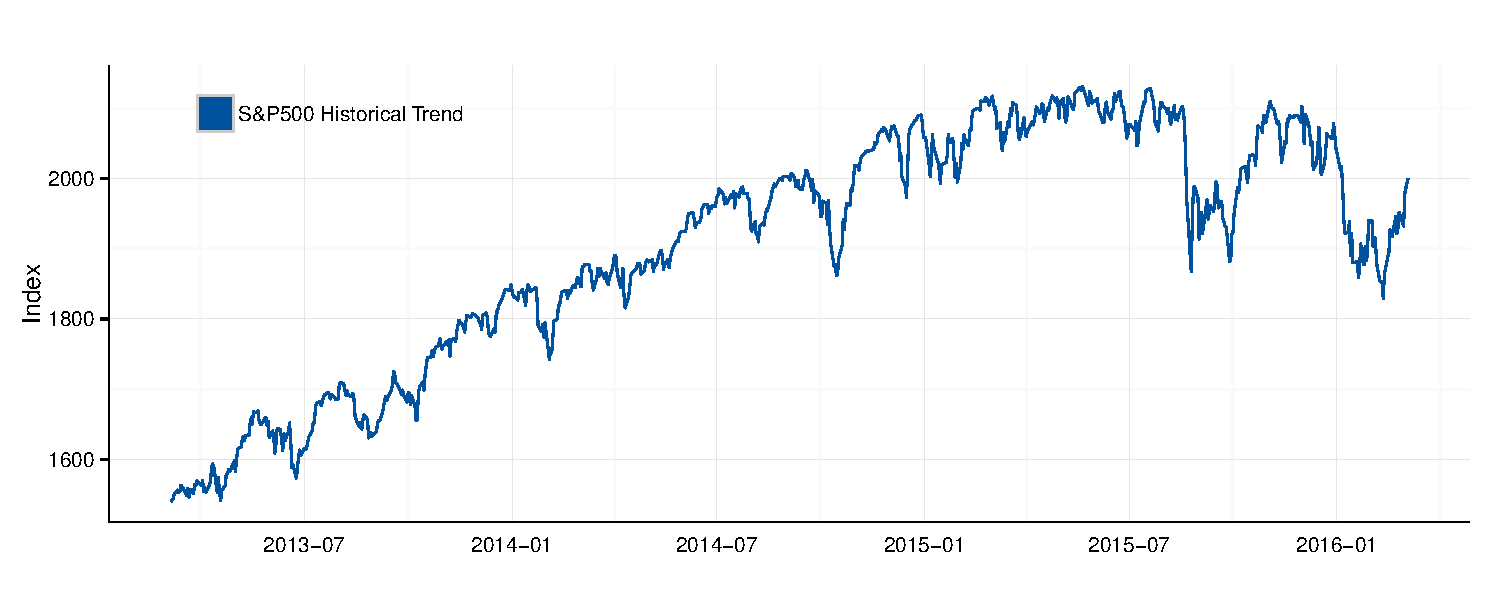
\includegraphics[width=\textwidth]{SP500/histFig1.pdf}
        \caption{S\&P 500 historical prices}
        \label{fig:SP:hist}
        \end{figure}
Sample data of S\&P 500 is composed of its daily close 
between Mar. $5^{th}$, 2013 and Mar. $4^{th}$, 2016
\footnote{Data source: Yahoo Finance},
i.e.\,757 prices within three years in total. 
Of all 757 records, two thirds of them (data before Mar. $6^{th}$, 2015) are used as in-sample data
for K-Means model training and HMM initialization. 
The remaining one third are reserved to compare with the simulated prediction results.

Illus.\,\ref{fig:SP:hist} presents the historical prices and trends of S\&P 500 during all three years. 
The index had been going up steadily, though with fluctuations, 
since the very beginning until around July, 2015. 
It then suffered a large downturn followed by a short period of turbulence, 
and then a large upgoing trend.
Generally speaking, the index presented quite different behaviors, 
in terms of both trend and volatility, between in-sample data and out-of-sample data.

        \begin{figure}[!hbt]
        \center
        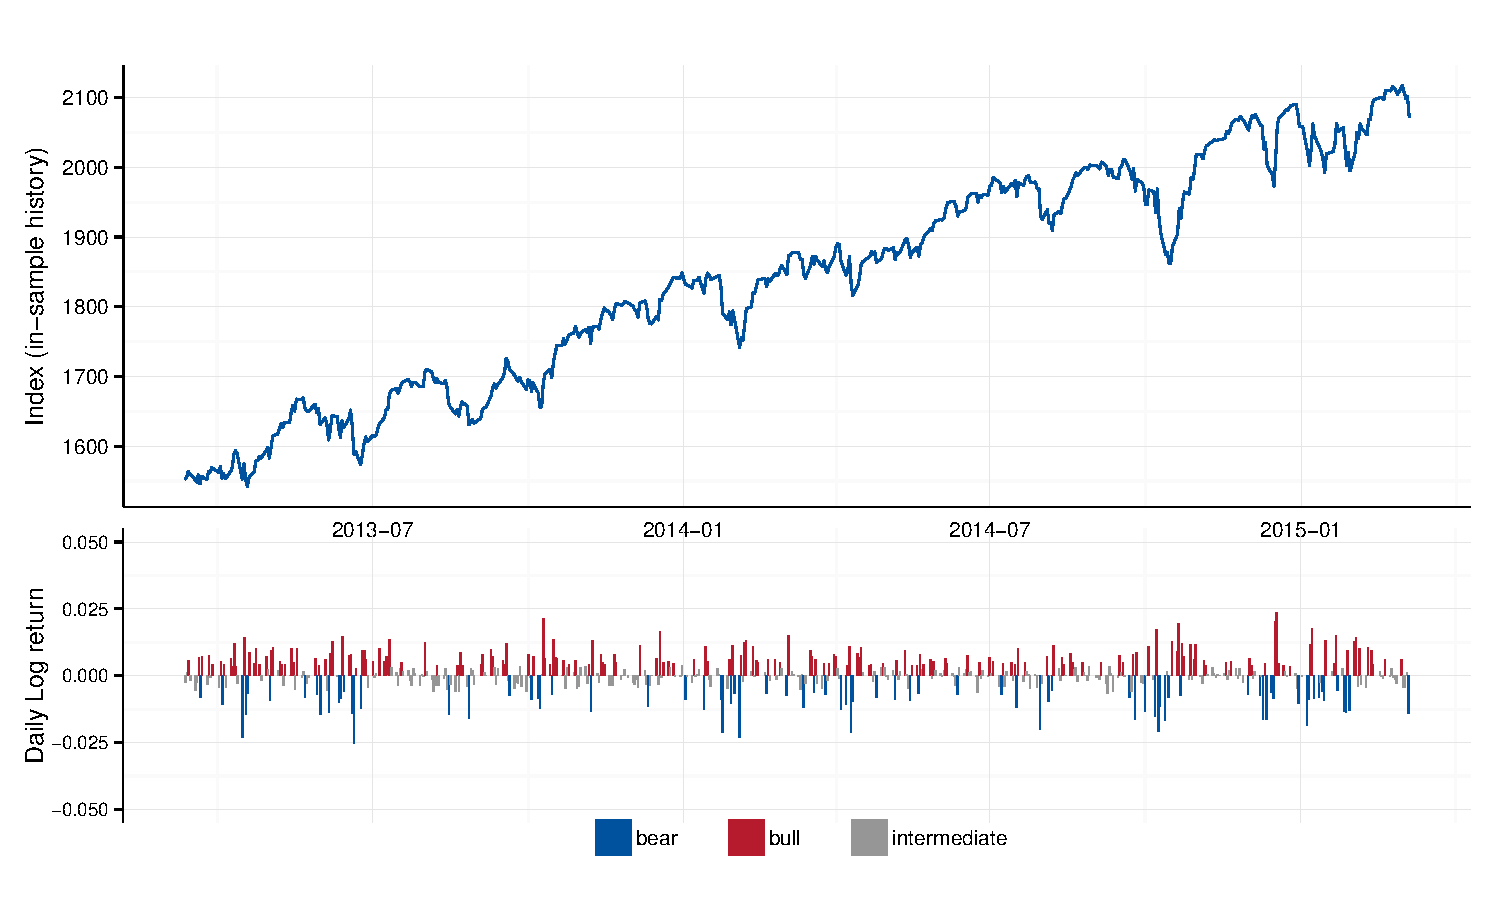
\includegraphics[width=\textwidth]{SP500/histFig3.pdf}
        \caption{S\&P in-sample trend with daily return bars}
        \label{fig:SP:histin}
        \end{figure}

        \begin{figure}[!hbt]
        \center
        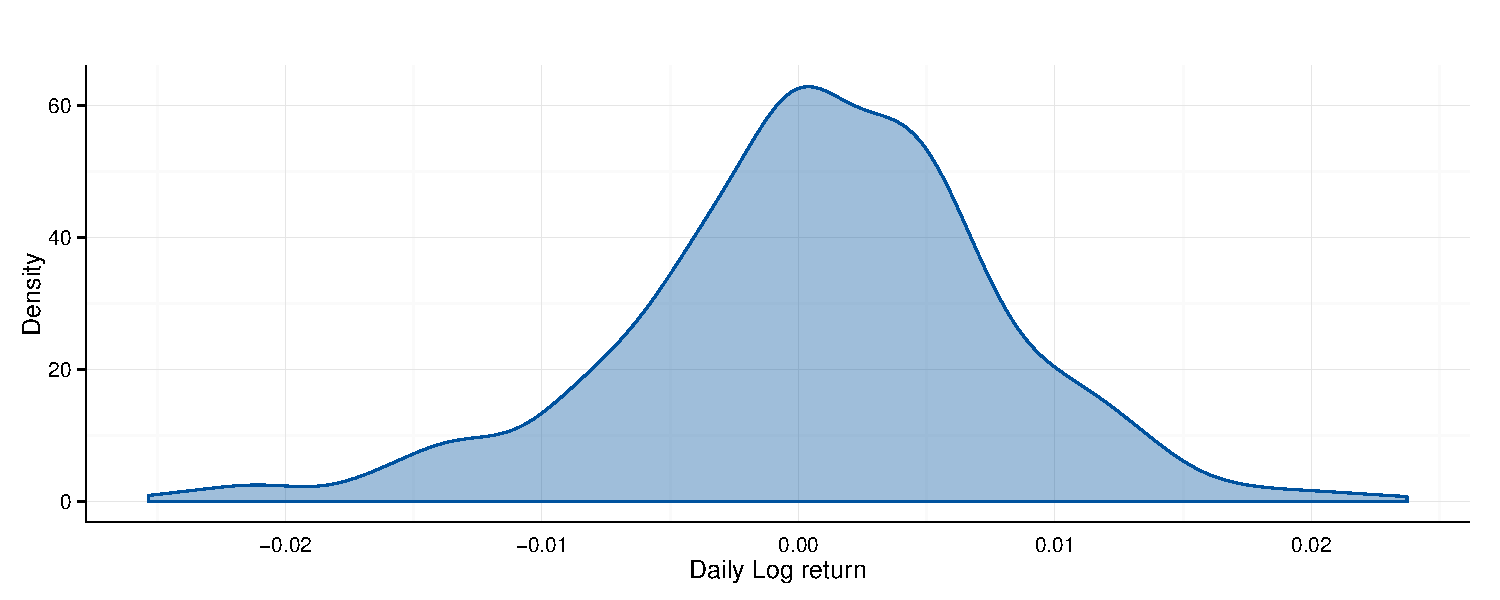
\includegraphics[width=\textwidth]{SP500/histFig4.pdf}
        \caption{Density distribution of S\&P in-sample daily returns}
        \label{fig:SP:ret}
        \end{figure}
Now take a look at the in-sample period.
Density distribution of daily returns is almost bell-curve shaped,
with slight skewness to the right (see Illus.\,\ref{fig:SP:histin} and \ref{fig:SP:ret}). 
Almost all returns are within the range $[-2.5\%,2.5\%]$ and 
with 5-day volatility less than $2\%$ (daily basis, indicated in Illus.\,\ref{fig:SP:KMeans}).

        \begin{figure}[!hbt]
        \center
        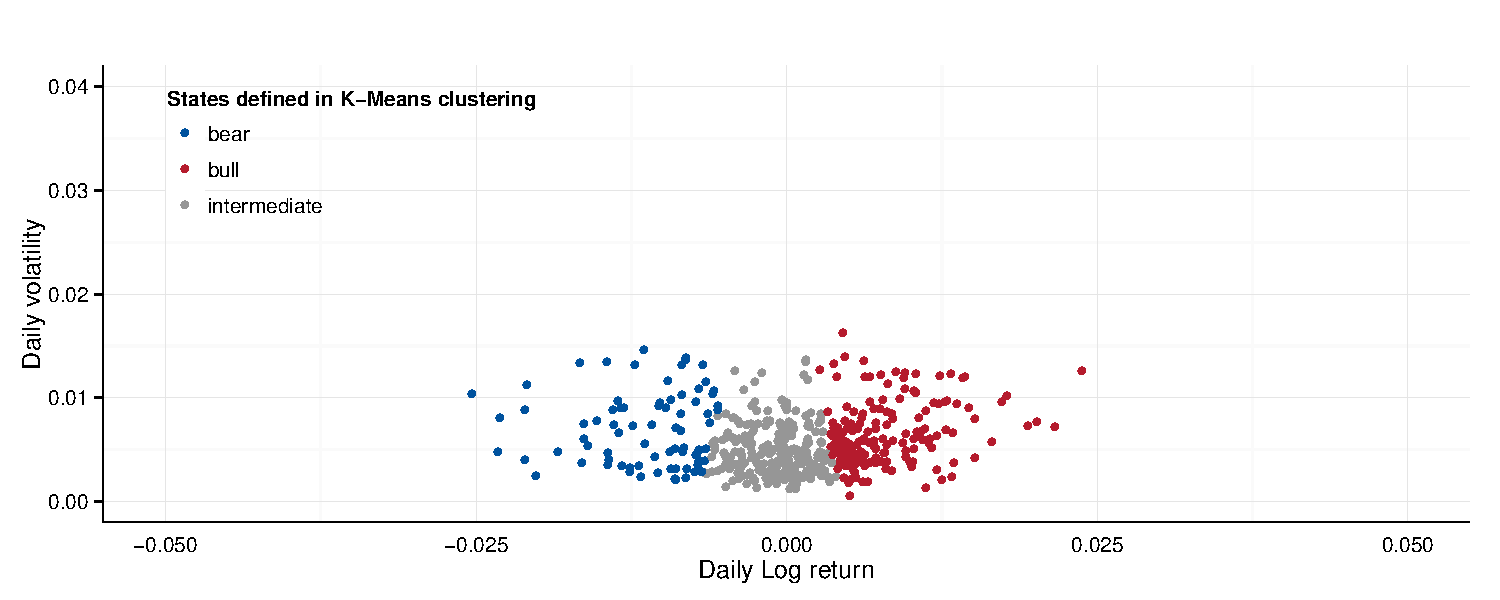
\includegraphics[width=\textwidth]{SP500/histFig2.pdf}
        \caption{K-Means result of S\&P 500 in-sample returns}
        \label{fig:SP:KMeans}
        \end{figure}
The result of K-Means clustering is pretty straightforward 
as it classifies the lowest one third of the returns as bear,
the highest one third as bull and the remaining as in the intermediate state.
Note that the clustering of K-Means method is purely based on quantitative differences of the data
(daily return and corresponding 5-day volatility in this case),
and has nothing to do with the market states then.
The definition and names of the states are artificially given to 
merely distinguish the three clustering centers.


\subsection{State transition parameters}
\label{sec:positive:SP:transition}
The three by three state transition matrix has nine unknown parameters in total,
estimated by EM algorithm through iteration.
Illus.\,\ref{fig:SP:transition} presents four chord plots
of the state transition matrix for S\&P 500 in-sample data.

        \begin{figure}[!hbt]
        \center
        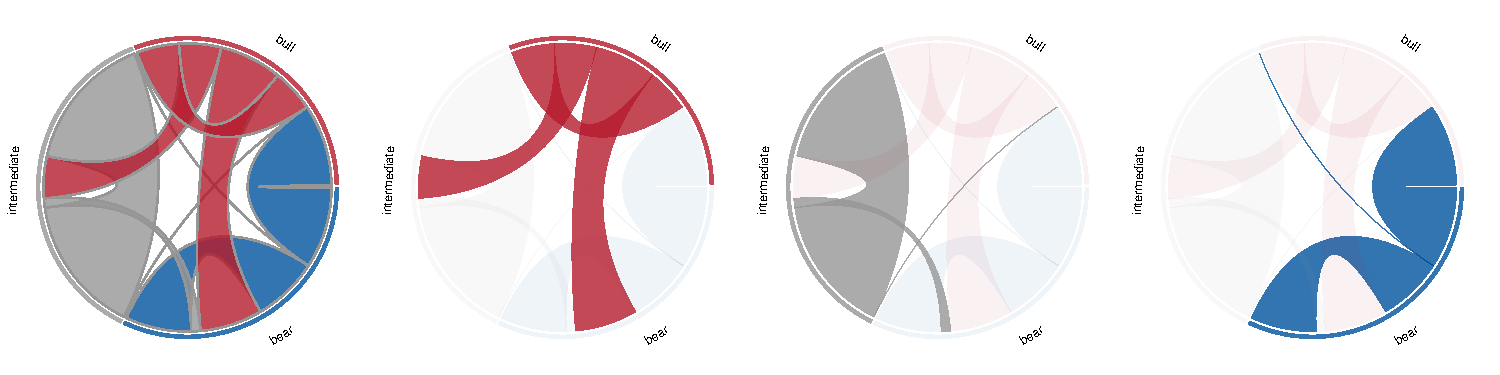
\includegraphics[width=\textwidth]{SP500/transFig1.pdf}
        \caption{State transition for S\&P 500 in-sample data}
        \label{fig:SP:transition}
        \end{figure}
The first plot in Illus.\,\ref{fig:SP:transition} visualizes a complete state transition matrix.
Three different colors each stands for a hidden state.
Every chord links two arcs:
the arc with the same color as the chord represents the current state,
and the other one represents the next state.
Since HMM allows for stays of the latent variable,
the state transition matrix may have non-zero diagonal entries,
leading to chords that travels from and to the same arc.

The latter three plots each shows the transition vector conditional on the current state.
As can be seen, a bull market is most likely to enter a bear state (with probability of $42\%$),
and to stay put or transit into an intermediate state with the same probability (of $29$\%).
However, a market at intermediate state stays at intermediate with great chance (about $93\%$),
but is almost impossible to change into a bull market (with probability less than $10^{-5}$).
A bear market, on the other hand, is more likely to transit into a bull than stay still 
with a slightly higher probability ($55\%$ vs. $45\%$) 
and has very little chance to go intermediate (with probability less than $10^{-6}$).
Transitions between extreme cases (bull and bear) seem more likely to happen,
compared to transitions between the intermediate state and an extreme case.

These patterns indicate a highly volatile market, 
where it is more possible to meet with a rebounce rather than a trend 
(except the intermediate state, which might represent lack of trends).
This fact can be indirectly proved by Illus.\,\ref{fig:SP:histin}.
The index kept going up for two years and the trend seems quite obvious;
but upturns and downturns, not only small waves but also large ones, 
are densely distributed within the period.
The volatility of the market will be more clear if one takes into account inflation.


\subsection{Conditional distribution parameters}
\label{sec:positive:SP:distribution}
Another type of unknown parameters are those of the Gaussian distributions 
conditional on each hidden state.
Conditional distribution parameters include three pairs of 
expectation and variance (or standard deviation).
The optimal estimation during each iteration can be analytically computed through EM
(see Sec.\,\ref{sec:HMM:EM}).

The estimation result of S\&P 500 in-sample is given as follow:
        \begin{equation}
        \left (
        \begin{array}{c c c}
        -1.13\%  &  -0.08\%  &  0.78\%  \\
         0.70\%  &   0.49\%  &  0.65\%  \\
        \end{array}
        \right ).
        \end{equation}
Each column in order represents the bear state, the intermediate and the bull.
Entries in the first row are corresponding expectations 
and ones in the second row are standard deviations.
It is clear that returns during the bear and bull 
have higher variances and non-zero expectations,
while returns during the intermediate are closer to zero and have lower volatility.

        \begin{figure}[!hbt]
        \center
        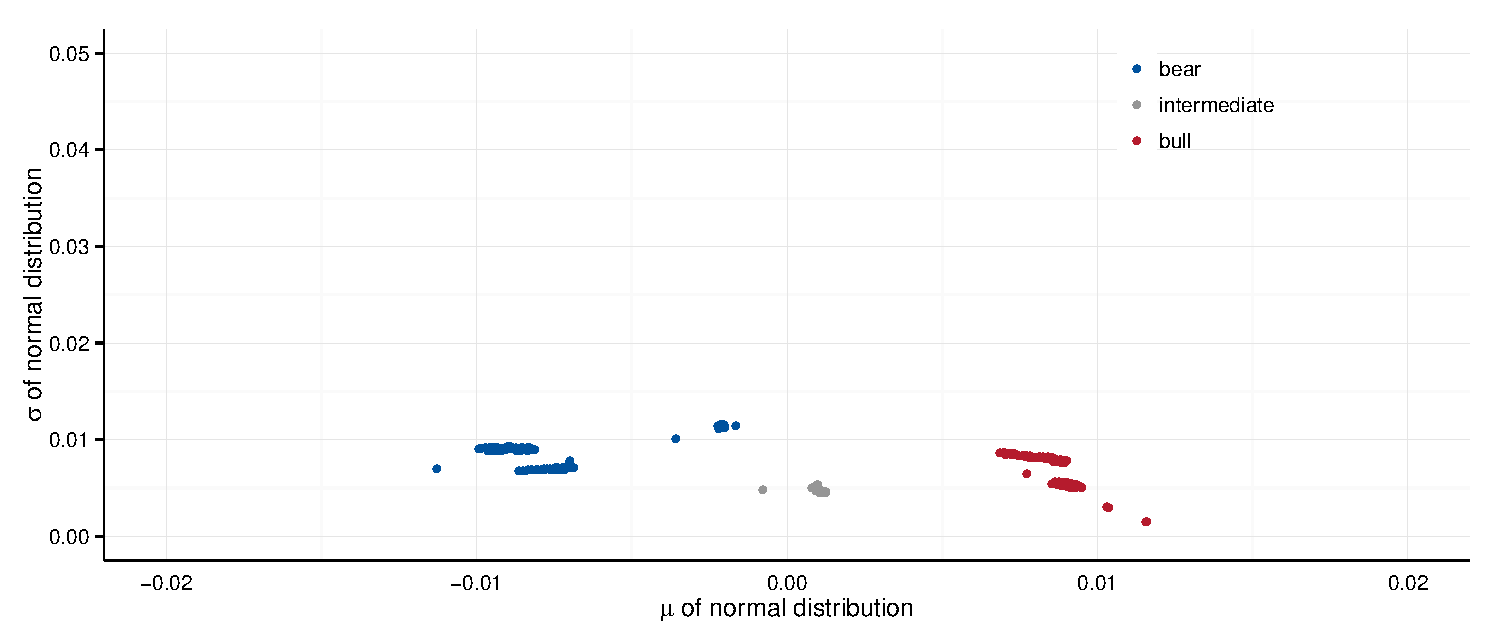
\includegraphics[width=\textwidth]{SP500/paramFig1.pdf}
        \caption{Conditional distribution parameters across time}
        \label{fig:SP:distscatter}
        \end{figure}
We also consider time-variation of the parameters.
As a matter of fact, when the simulated prediction is processing,
more information has been incorporated into the model and parameters change with time.
Illus.\,\ref{fig:SP:distscatter} and \ref{fig:SP:distdist} are to 
describe the conditional distribution parameters time series.

The aforementioned patterns about the parameters remain across time.
Bear(bull) states have expected returns significantly below(over) zero and higher volatility,
while intermediate states have expectations around zero and a relatively lower volatility.
Notice that some distributions conditional on bull states also have smaller variance,
indicating a slower and milder rise.
Clearly bears always come more strongly.

        \begin{figure}[!hbt]
        \center
        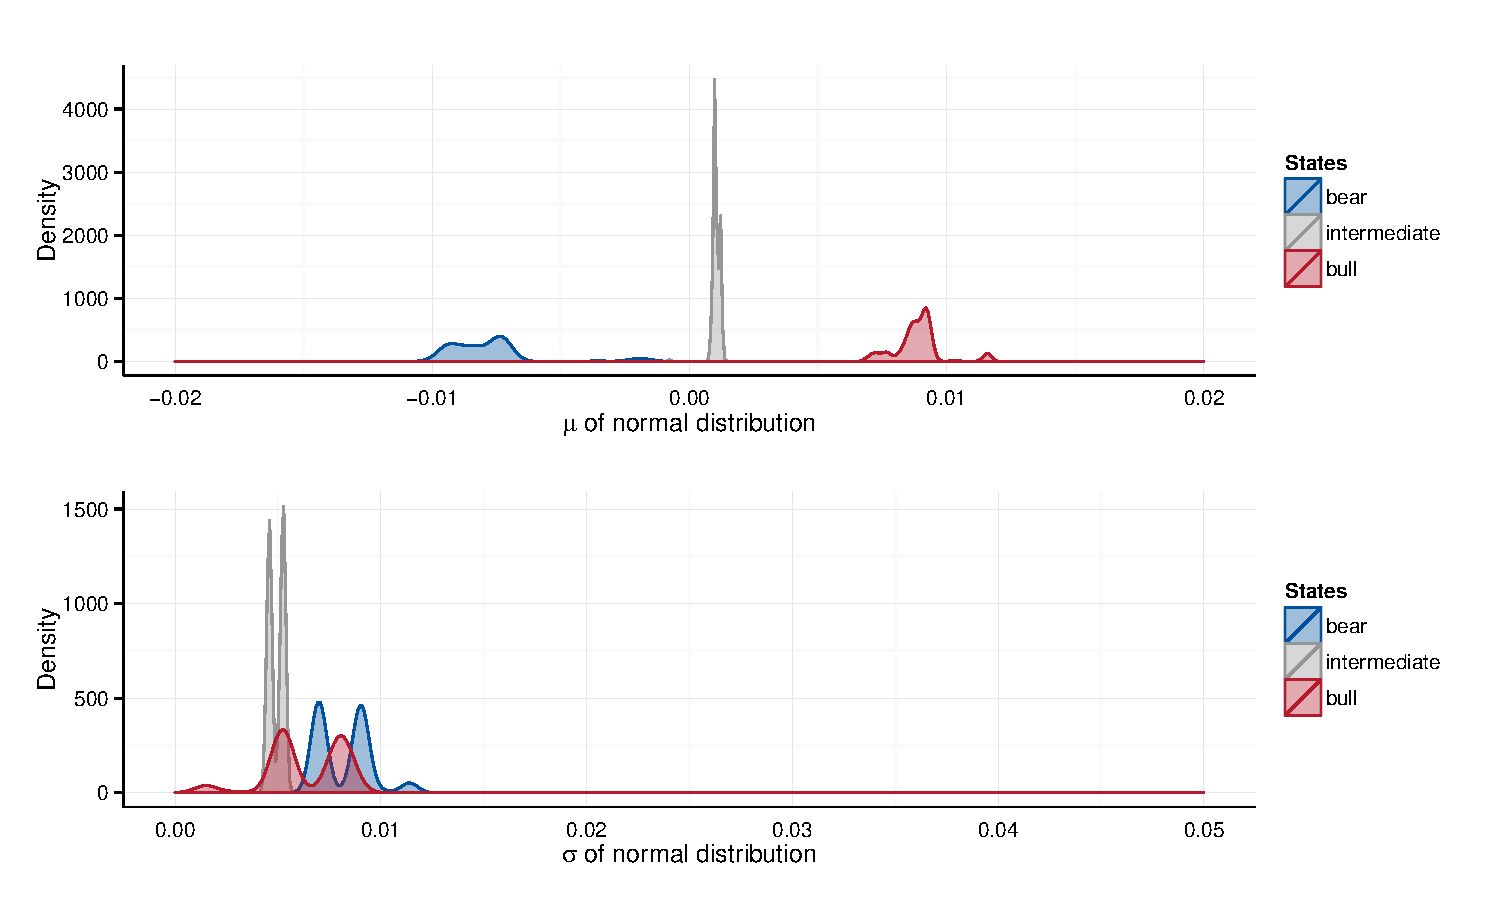
\includegraphics[width=\textwidth]{SP500/paramFig2.pdf}
        \caption{Density distribution of conditional distribution parameters}
        \label{fig:SP:distdist}
        \end{figure}
Illus.\,\ref{fig:SP:distdist} shows the density distribution of these parameters.
The multi-modality of $\sigma$ matches the multi-clustering-center in Illus.\,\ref{fig:SP:distscatter}.
Therefore, chances are that even the same hidden state presents different behaviors.
It means it might be necessary to increase the number of hidden states in the model,
which is currently against Assumption \ref{asp:states} and 
will be discussed about in Sec.\,\ref{sec:positive:result:states}.


\subsection{Global decoding and hidden states}
\label{sec:positive:SP:states}

        \begin{figure}[!hbt]
        \center
        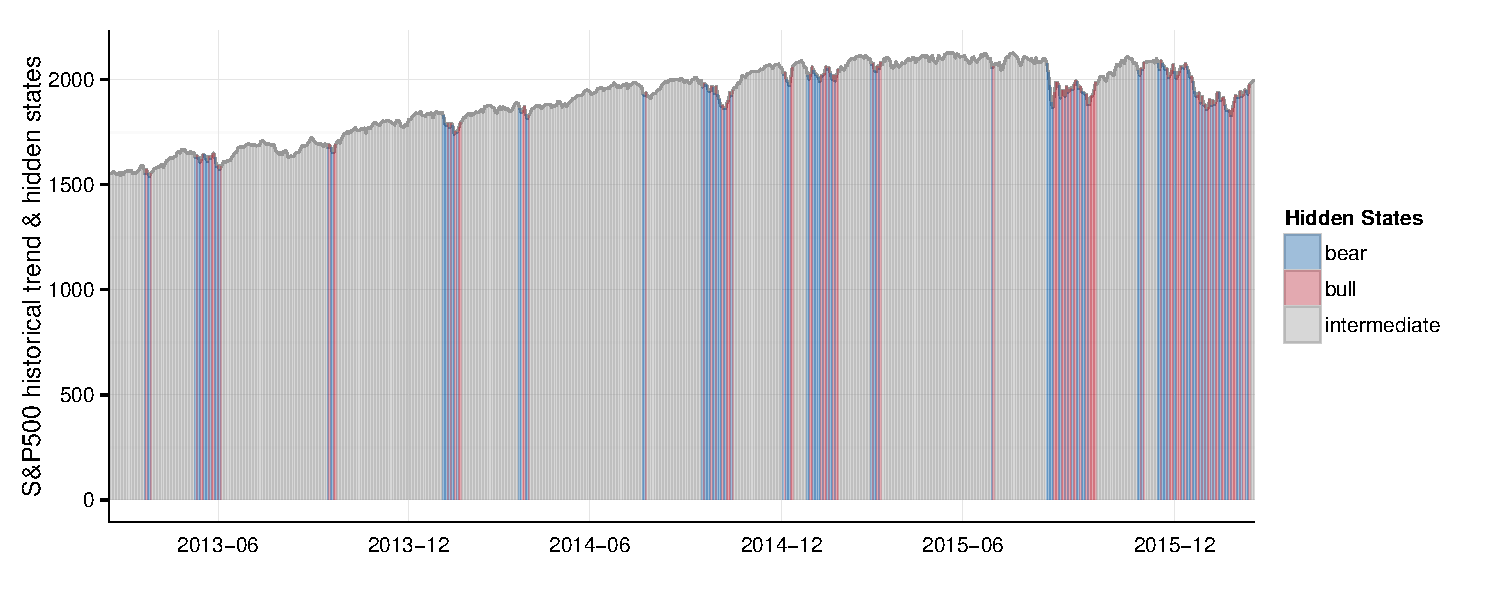
\includegraphics[width=\textwidth]{SP500/statesFig1.pdf}
        \caption{S\&P 500 in-sample trend and states sequence}
        \label{fig:SP:seqstates}
        \end{figure}
Global decoding based on Viterbi algorithm enables us to find the 
most probable sequence of hidden states,
which shall help us learn about the market with ability to 
identify the market states during the observation period.

Illus.\,\ref{fig:SP:seqstates} provides knowledge about 
the sequence of hidden states of S\&P 500 in-sample data.
The color gray, standing for the intermediate state, 
makes up the majority of the figure.
Bears and bulls are far less frequent than intermediates and often come together.
This phenomenon is better expressed by Illus.\,\ref{fig:SP:states}

        \begin{figure}[!hbt]
        \center
        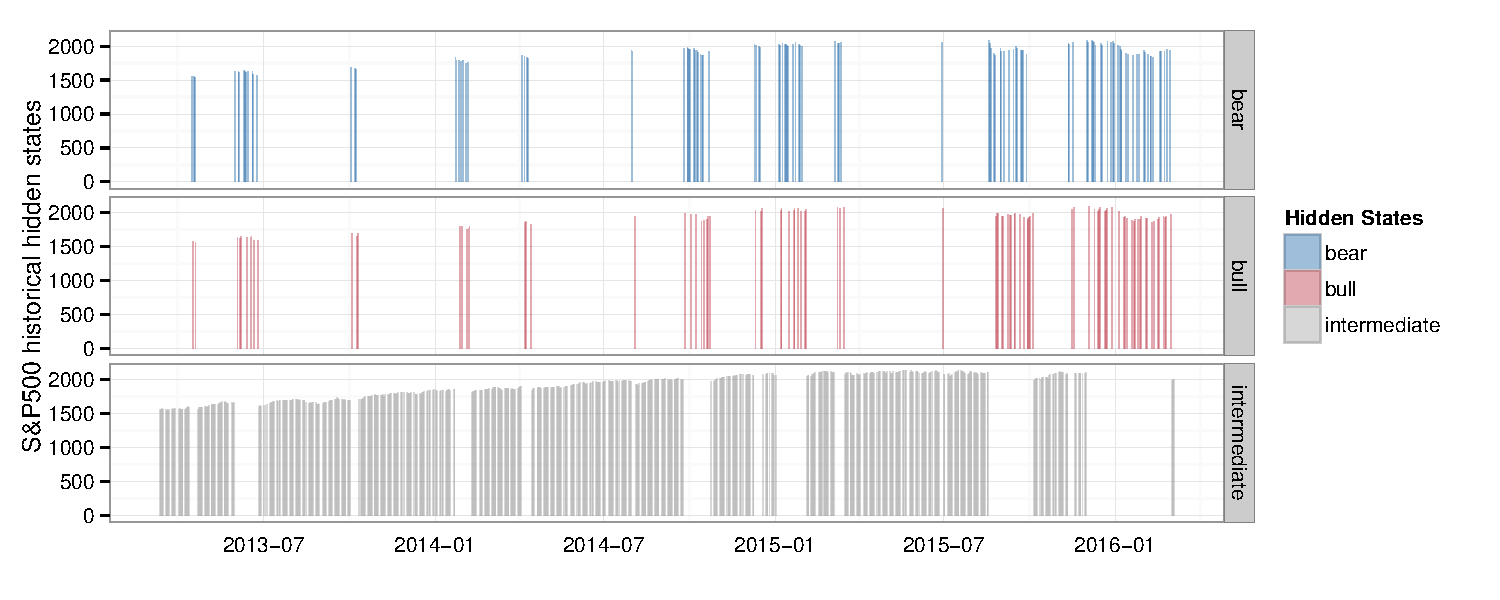
\includegraphics[width=\textwidth]{SP500/statesFig2.pdf}
        \caption{S\&P 500 historical hidden states}
        \label{fig:SP:states}
        \end{figure}
The upper two parts of Illus.\,\ref{fig:SP:states} are almost the same except for color labels,
which proves the closeness of bears and bulls.

Actually the global decoding result also supports, from a visual perspective, 
our findings mentioned in Sec.\,\ref{sec:positive:SP:transition},  
that extreme states tend to transit into each other instead of the intermediate.

        \begin{figure}[!hbt]
        \center
        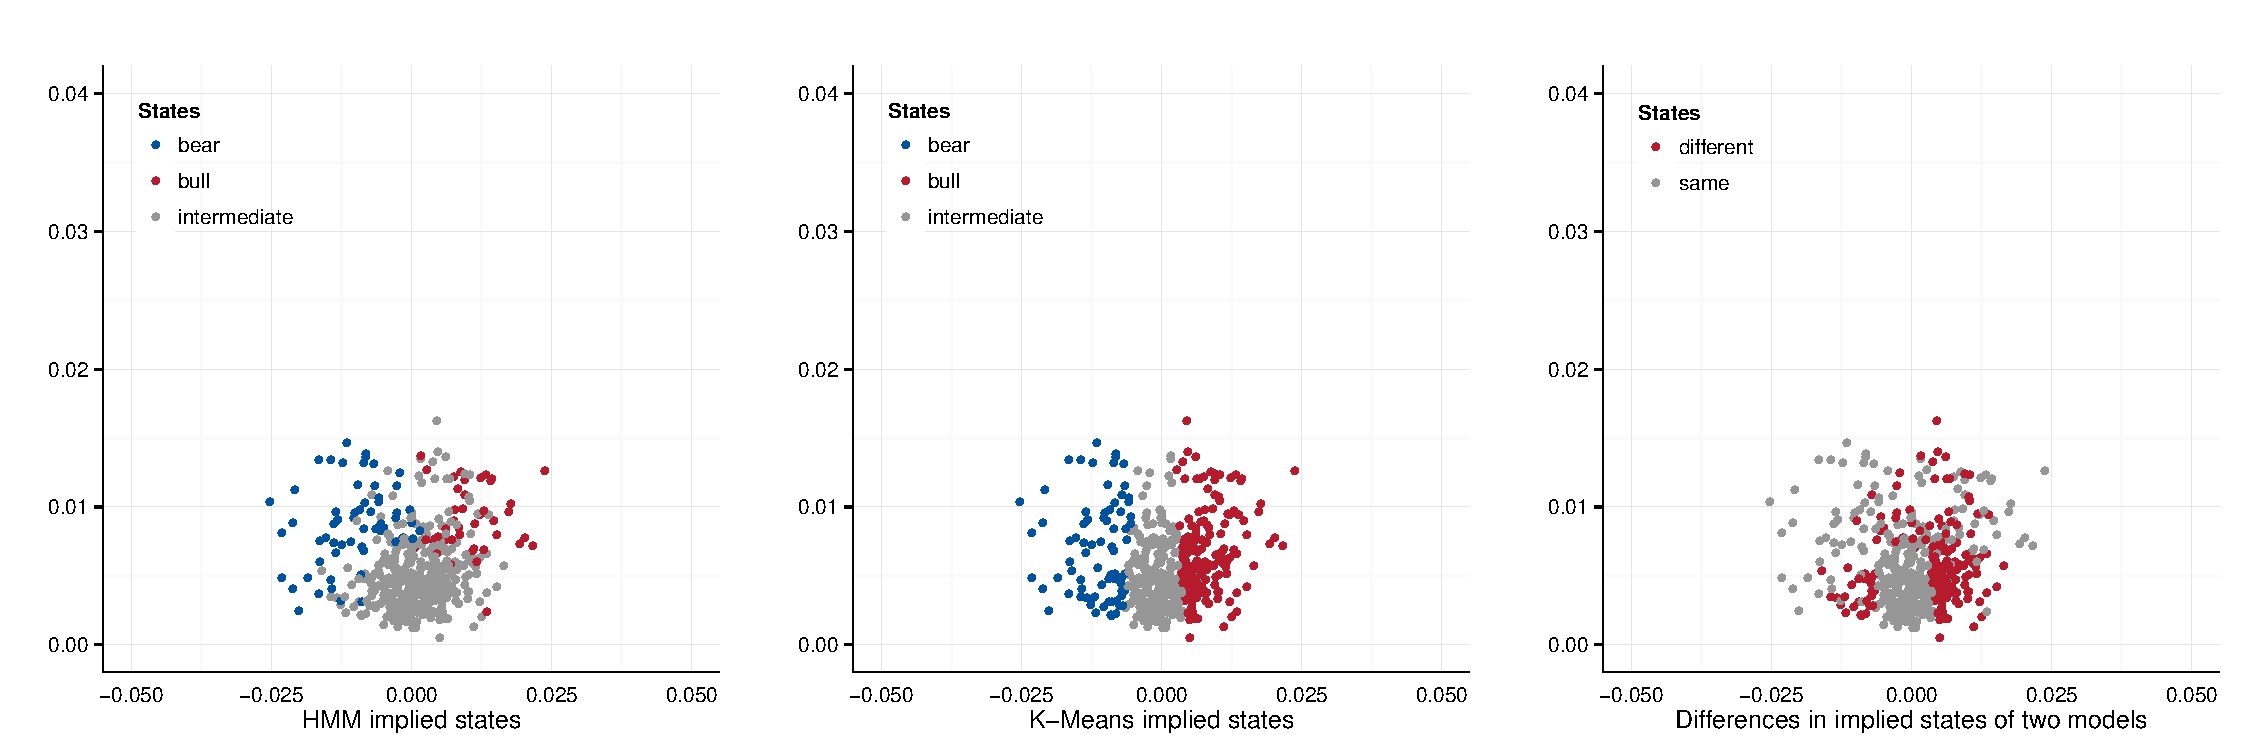
\includegraphics[width=\textwidth]{SP500/statesFig3.pdf}
        \caption{Comparison between K-Means states and HMM hidden states}
        \label{fig:SP:diffstates}
        \end{figure}
Illus.\,\ref{fig:SP:diffstates} shows the states of in-sample returns implied by HMM and K-Means.
As we mentioned before, K-Means distinguish the states based merely on 
quantitative properties of the data, not taking into account their correlations and transitions.
Hence, most of the differences lie in the bull zone in K-Means, 
which are identified as intermediate in HMM.
Statistically speaking, these returns are relatively higher,
but they are more likely to appear during an intermediate state according to HMM.
It is similar for those which are labeled as bear in K-Meas but intermediate in HMM.
There also exist some points classified as intermediate in K-Means 
but considered to be in one of the extreme states in HMM.
These points may be viewed as small adjustments (or small rebounces) under a big trend,
even though they are close to zero.


\subsection{Simulated prediction results}
\label{sec:positive:SP:prediction}
Simulated prediction is carried out on out-of-sample data and 
the model is updated on a daily basis.
Information of the real historical daily return is incorporated into 
the current model in order to predict the return for the next day.
Illus.\,\ref{fig:SP:predictionall} presents the result of the prediction
over the entire observation period (in-sample and out-of-sample).
Predicted returns are cumulatively summed and taken exponential, 
multiplied by the first closing price of the out-of-sample data.

        \begin{figure}[!hbt]
        \center
        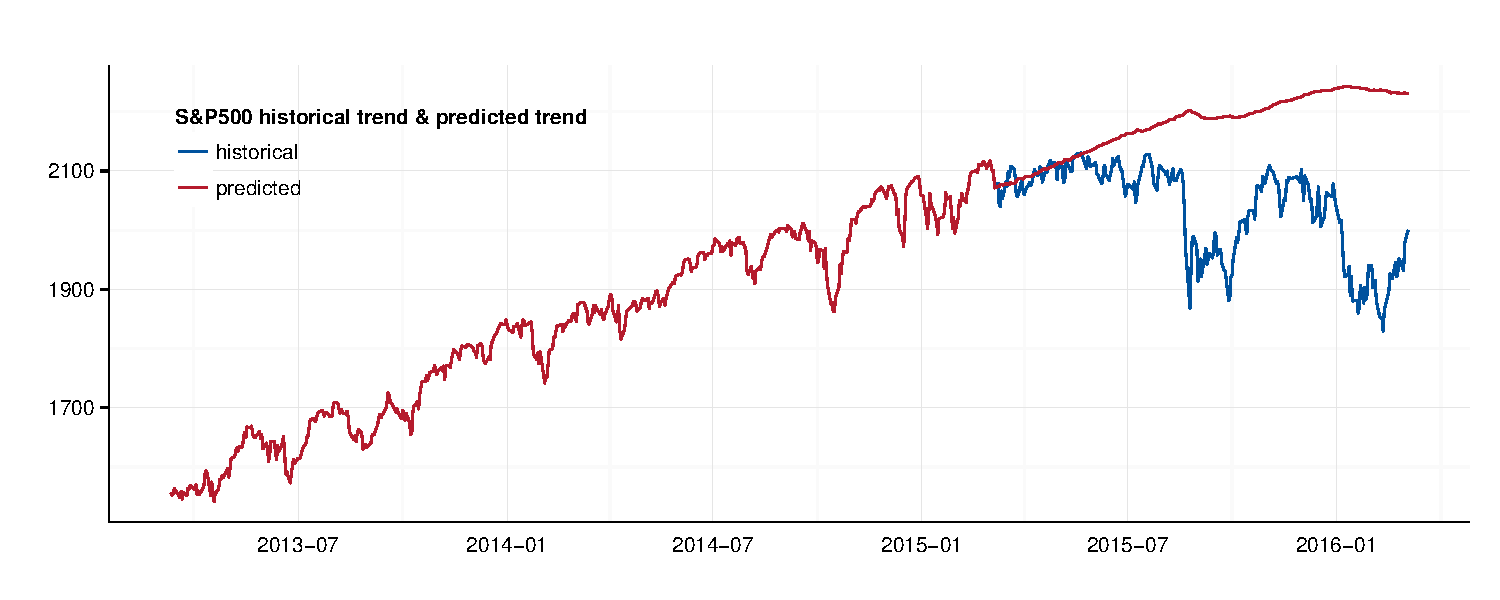
\includegraphics[width=\textwidth]{SP500/predictionFig1.pdf}
        \caption{S\&P 500 simulated prediction result}
        \label{fig:SP:predictionall}
        \end{figure}
Visually speaking the prediction result is extremely poor.
The predicted result preserves the trend of the in-sample data
and has started to deviate from the real history since June 2015.

        \begin{figure}[!hbt]
        \center
        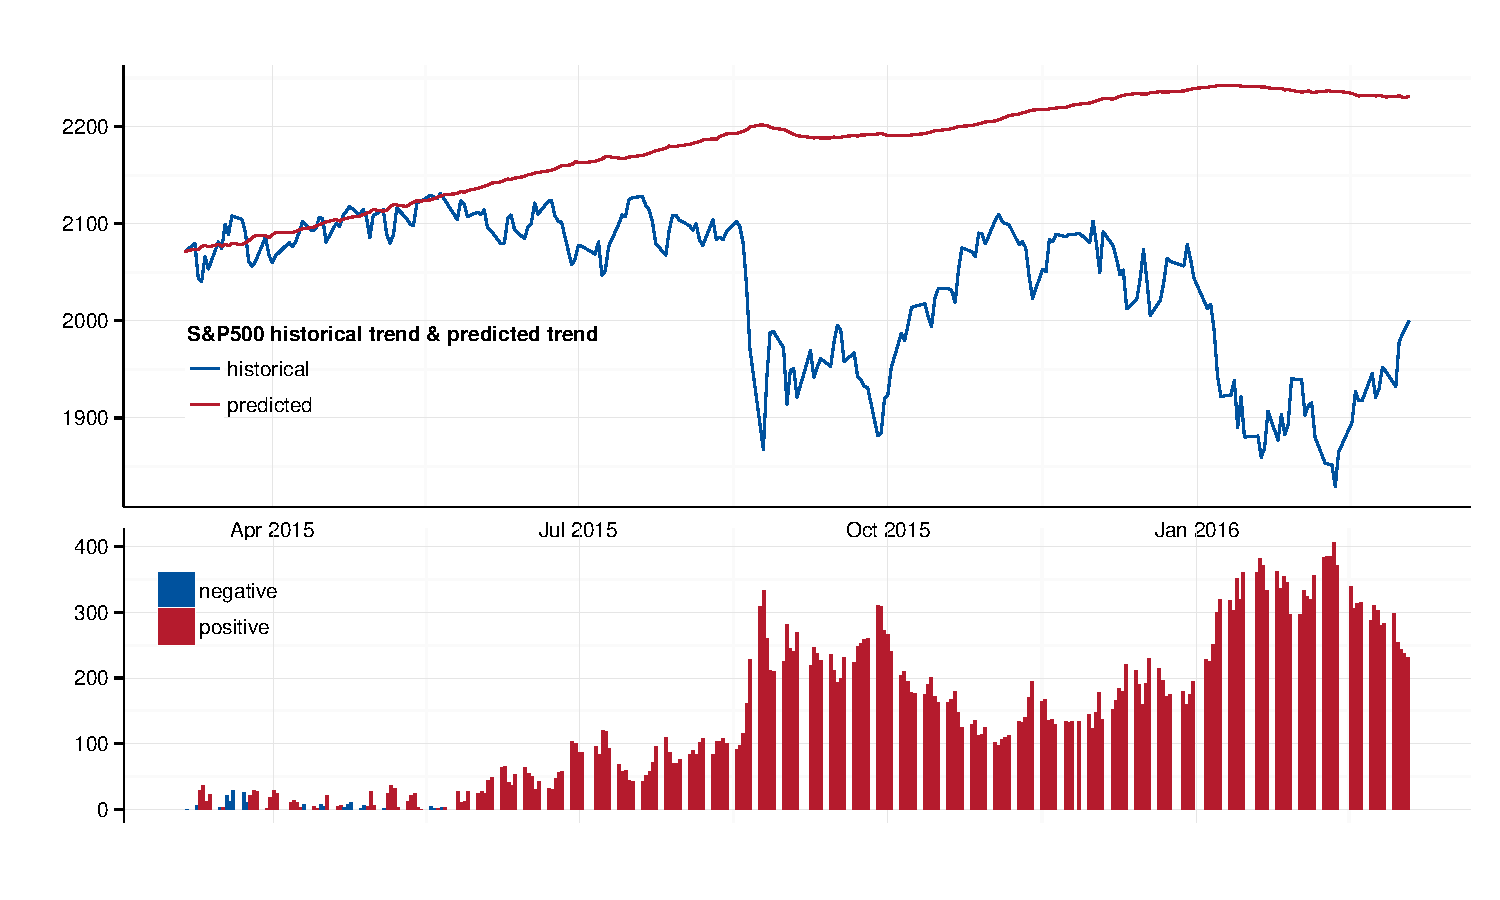
\includegraphics[width=\textwidth]{SP500/predictionFig2.pdf}
        \caption{S\&P 500 simulated prediction result out-of-sample part}
        \label{fig:SP:predictionout}
        \end{figure}
Illus.\,\ref{fig:SP:predictionout} shows both the trend and differences 
between the historical value and the prediction result.
Difference shot up when the index changed from a up-going trend to a downward shape.
Illus.\,\ref{fig:SP:predictionstd} indicates that even considering the standard deviations 
cannot help with the prediction.

        \begin{figure}[!hbt]
        \center
        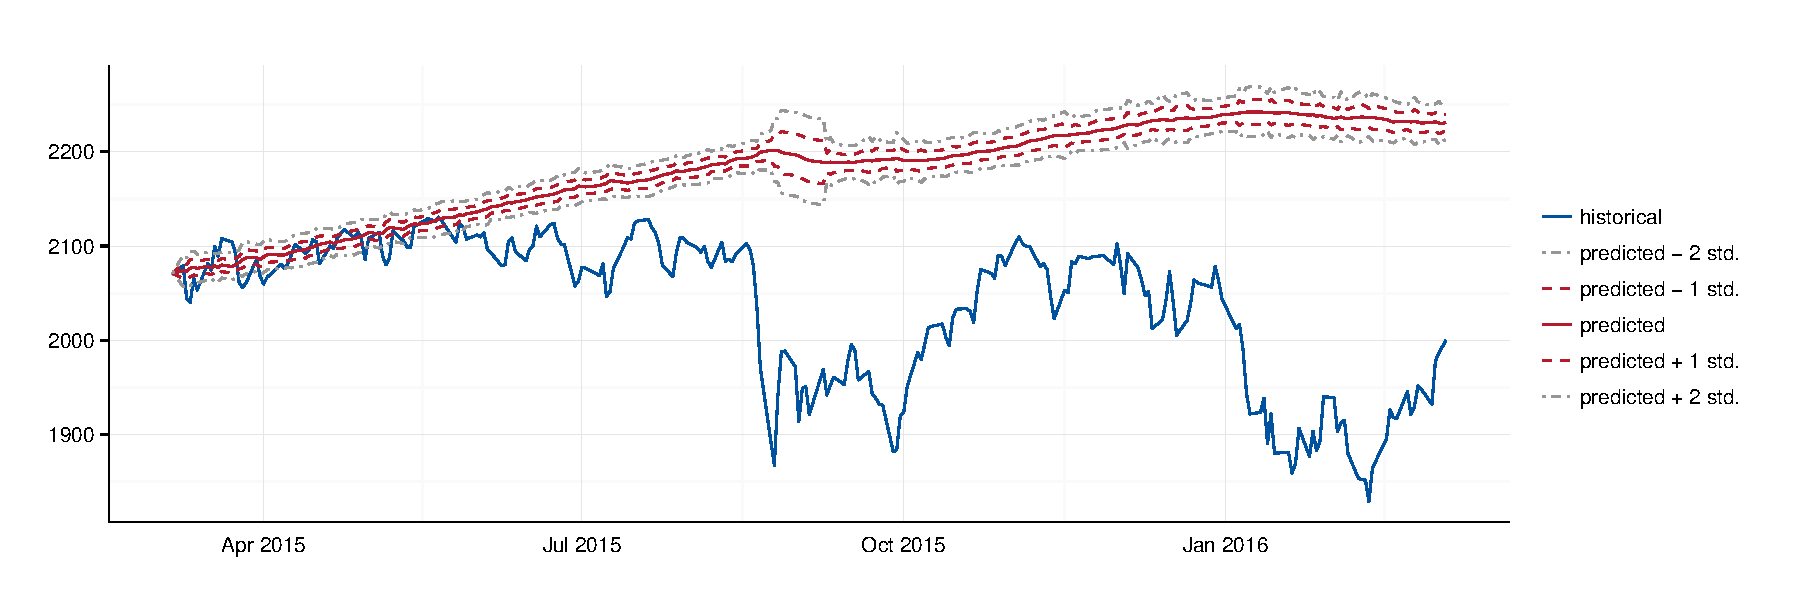
\includegraphics[width=\textwidth]{SP500/predictionFig3.pdf}
        \caption{S\&P 500 simulated prediction result with confidence band}
        \label{fig:SP:predictionstd}
        \end{figure}
However, the simulated prediction result has a win ratio of $50.4\%$,
which means the model has predicted the right direction of the index 
with probability slightly over a half.

Besides, as we mentioned in the very beginning of Sec.\,\ref{sec:positive:SP:prediction},
the predicted curve is based on the first closing price of the out-of-sample data 
but does not consider the current price of the index.
The most direct and obvious result of such a method is that prediction errors accumulate,
leading to larger and larger deviation from the real history.

        \begin{figure}[!hbt]
        \center
        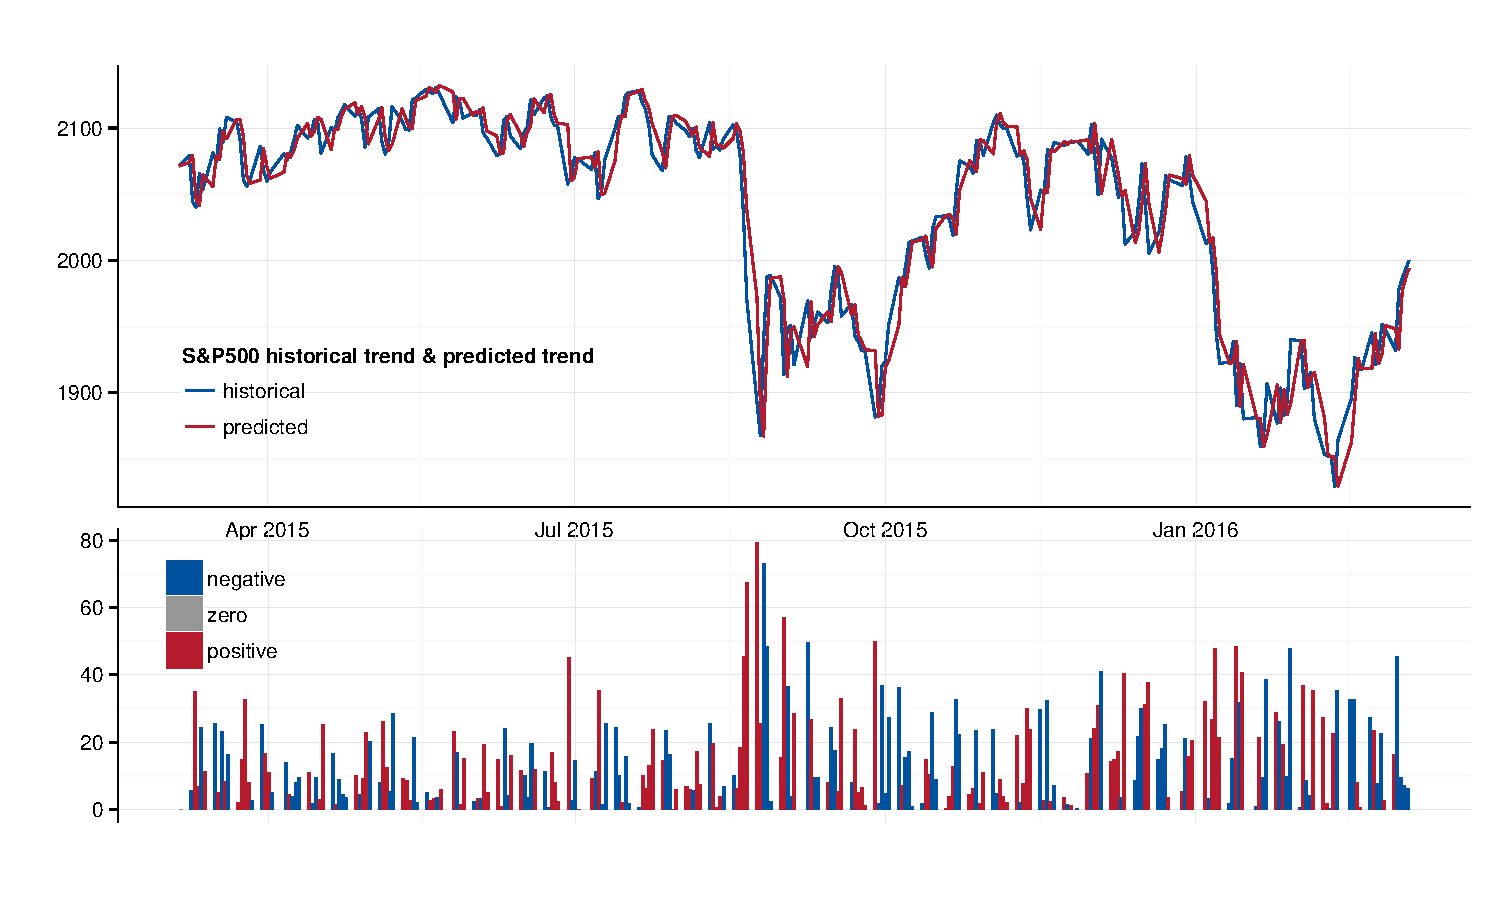
\includegraphics[width=\textwidth]{SP500/predictionFig4.pdf}
        \caption{S\&P 500 adaptive prediction}
        \label{fig:SP:predictiondyn}
        \end{figure}
Therefore, it is reasonable to fully use the information provided by the data,
including both real returns and real closing prices.
We base prediction for the next day on both return and closing price at the standing point,
and the result seems much better, as shown in Illus.\,\ref{fig:SP:predictiondyn}.
Illus.\,\ref{fig:SP:predictiondynstd} plots the result and index along with 
$\pm \sigma, \pm 2\sigma$ bands.
The real index is almost entirely covered by the $\pm 2\sigma$ band,
which stands for a $95.45\%$ confidence interval of prediction.

        \begin{figure}[!hbt]
        \center
        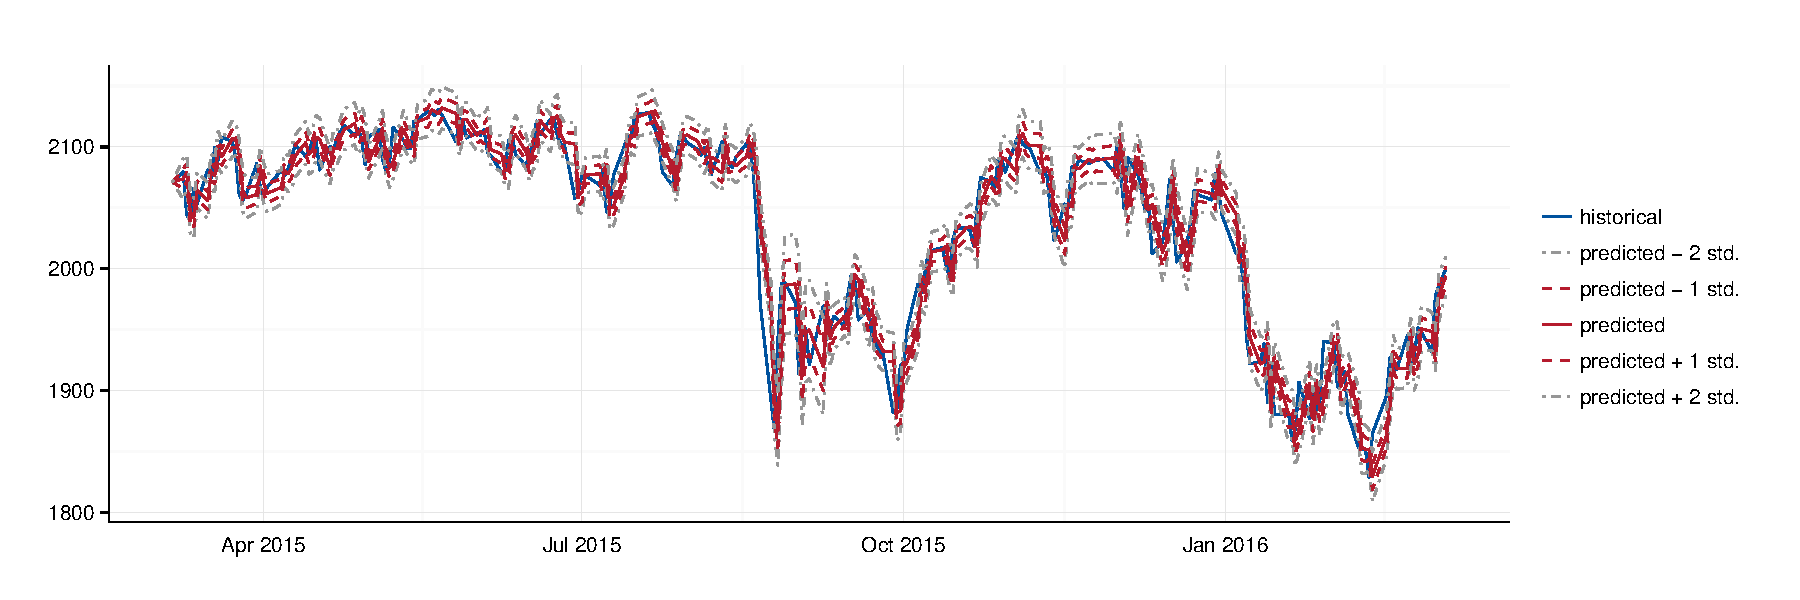
\includegraphics[width=\textwidth]{SP500/predictionFig5.pdf}
        \caption{S\&P 500 adaptive prediction with confidence band}
        \label{fig:SP:predictiondynstd}
        \end{figure}
It is worth noticing that there are clearly lags 
in the prediction results compared to the real index.
The extension of previous trend in Illus.\,\ref{fig:SP:predictionall} can be viewed
as a stronger version of such lag.
Furthermore, the lagging effect is not relived as time goes by,
but, on the opposite, exacerbated.

Thus, Conjecture \ref{conj:lag} seems reasonable to explain the phenomenon,
that too much outdated information is included and causes the lag and error.
Previous trends extend and too few weights have been allocated for the status quo.
More detailed analysis and explanations will be discussed in 
both Sec.\,\ref{sec:positive:result:prediction} and Sec.\,\ref{sec:future:lag}.

%%%%%%%%%%%%%%%%%%%%%%%%%%

\section{Chinese CSI 300 Index daily return series}
\label{sec:positive:CSI}
Of all stock market indices like Shanghai Composite Index, CSI 500 and CSI 800, etc.,
CSI 300 is the most typical and used for analysis.

\subsection{Data preprocessing and description}
\label{sec:positive:CSI:data}

        \begin{figure}[!hbt]
        \center
        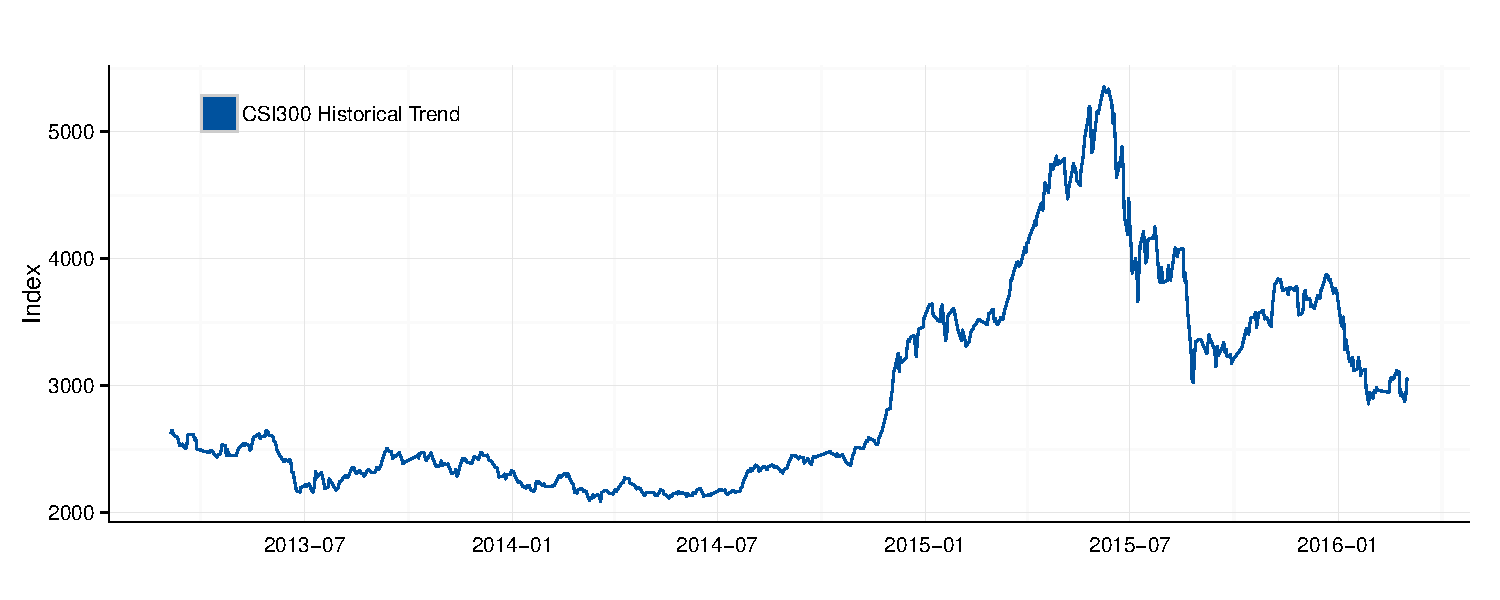
\includegraphics[width=\textwidth]{daily/histFig1.pdf}
        \caption{CSI 300 historical prices}
        \label{fig:CSI:hist}
        \end{figure}
Sample data of CSI 300 is selected between Mar.\,$5^{th}$, 2013 and Mar.\,$3^{rd}$, 2016
\footnote{Data source: Wind. All data of CSI 300, 
with different frequencies, are from the same data source},
totally 729 prices within three years, 
of which two thirds are used as in-sample, similar to the scheme in Sec.\,\ref{sec:positive:SP}. 
The time period is chosen as the same to the S\&P 500 case as well
so that the results are comparable.

As is shown in Illus.\,\ref{fig:CSI:hist},
the index was almost flat during 2013 and 2014 and met its big upturn at the end of 2014.
The big rise came in two parts and reached peak in May 2015,
followed by a rapid and large fall.
Rebounce occurred around September 2015 and then came another downturn in December.

        \begin{figure}[!hbt]
        \center
        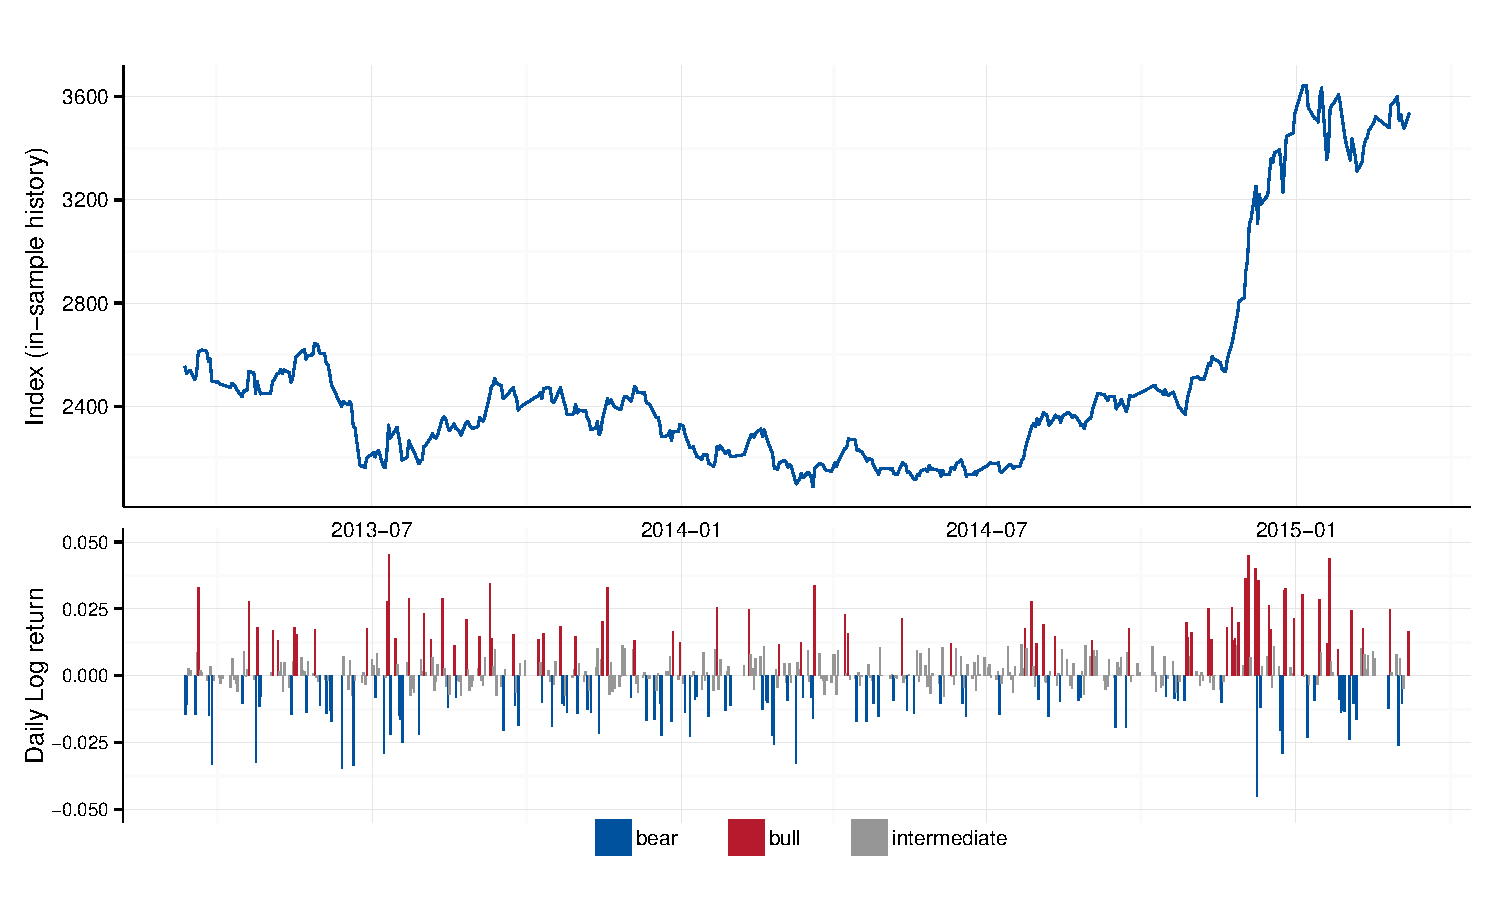
\includegraphics[width=\textwidth]{daily/histFig3.pdf}
        \caption{CSI 300 in-sample trend with daily return bars}
        \label{fig:CSI:histin}
        \end{figure}

        \begin{figure}[!hbt]
        \center
        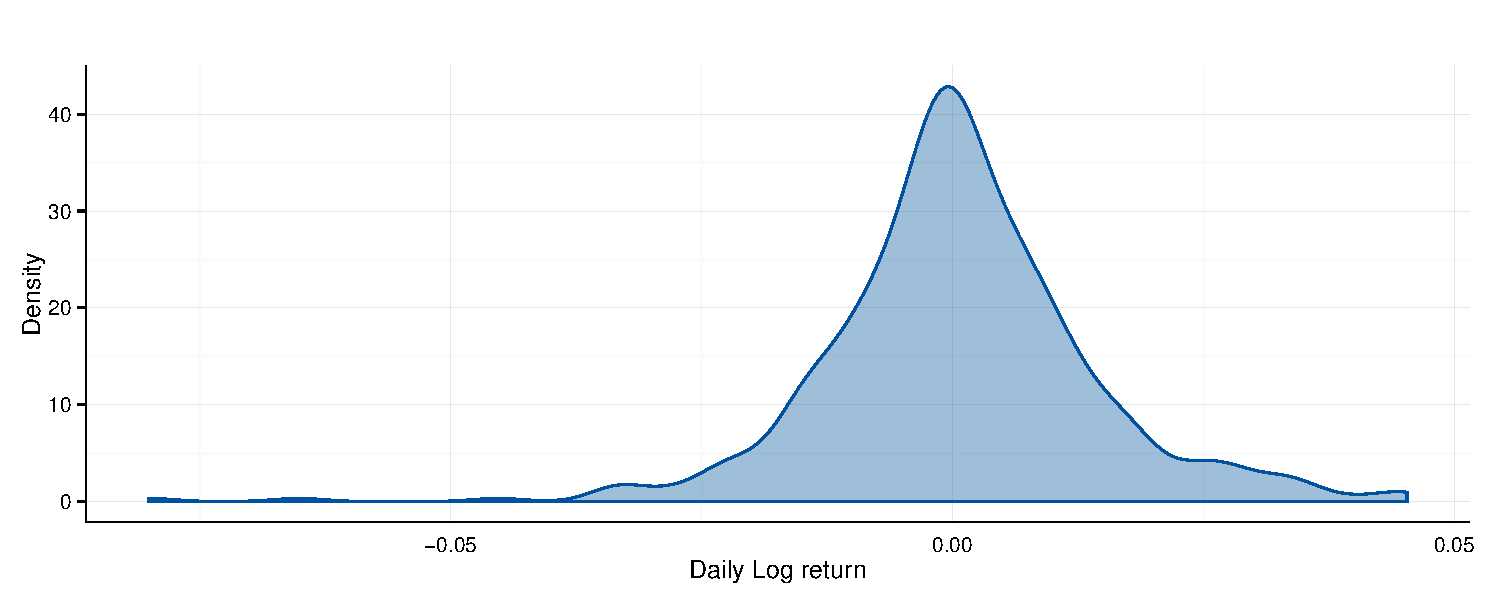
\includegraphics[width=\textwidth]{daily/histFig4.pdf}
        \caption{Density distribution of CSI 300 in-sample daily returns}
        \label{fig:CSI:ret}
        \end{figure}
The long period of fluctuation and almost half of the upgoing period
makes up the in-sample period.
Density distribution of daily returns has a lower skewness than S\&P 500 in-sample data,
but a longer tail on the left.

\subsection{State transition parameters}
\label{sec:positive:CSI:transition}
State transition matrix of CSI 300 data is quite similar to 
the one in Sec.\,\ref{sec:positive:SP:transition} but different in exact numbers.

        \begin{figure}[!hbt]
        \center
        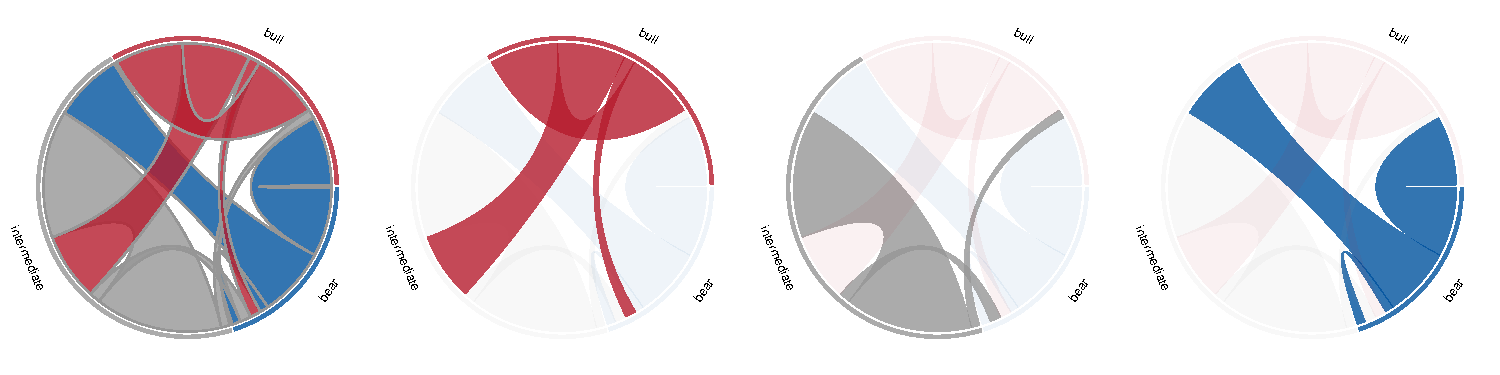
\includegraphics[width=\textwidth]{daily/transFig1.pdf}
        \caption{State transition for CSI 300 in-sample data}
        \label{fig:CSI:transition}
        \end{figure}
Illus.\,\ref{fig:CSI:transition} implements a similar chord diagram to 
visually present the transition matrix.
A bull market tends to stay at bull or transit into an indermediate with the same probability ($46\%$)
and is relatively unlikely to go into a bear directly.
An intermediate market has the chance of $86\%$ to stay put and 
a slightly higher probability to go into bear ($7.7\%$).
However, a bear market is very likely to get off the status quo,
with a probability of $47\%$ to turn into an intermediate and 
$46$ to even go into a bull directly.
This pattern is quite different from one in the U.S. market.

        \begin{figure}[!hbt]
        \center
        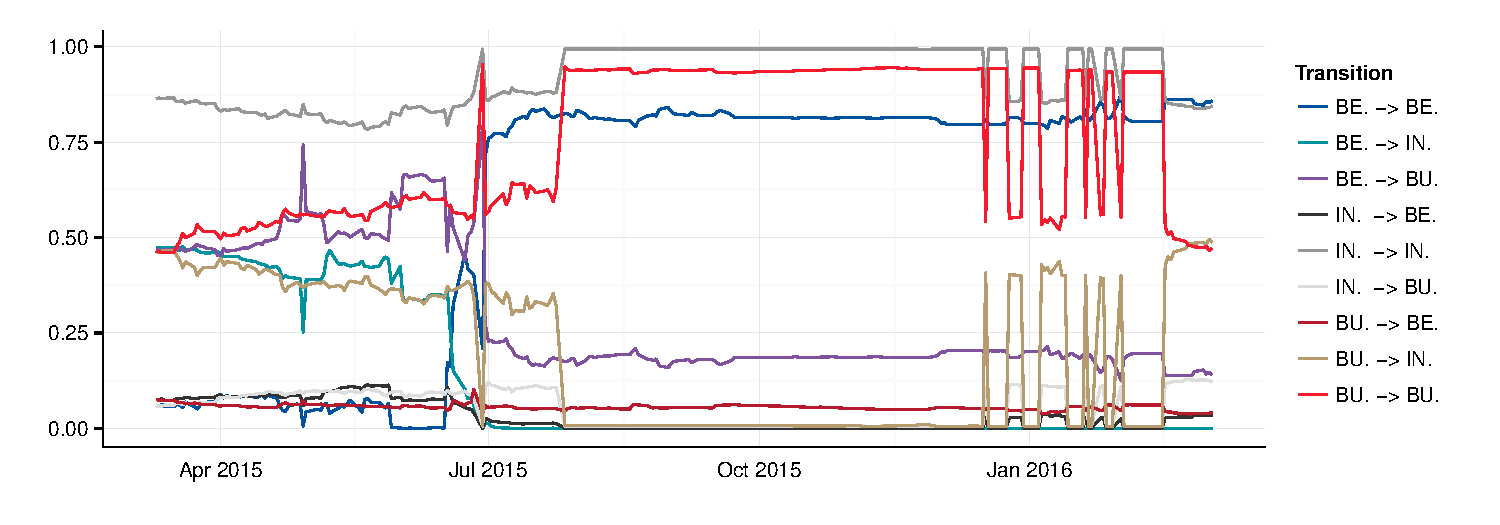
\includegraphics[width=\textwidth]{daily/transFig2.pdf}
        \caption{Evolution of state transition matrix entries}
        \label{fig:CSI:transitionevo}
        \end{figure}

        \begin{figure}[!hbt]
        \center
        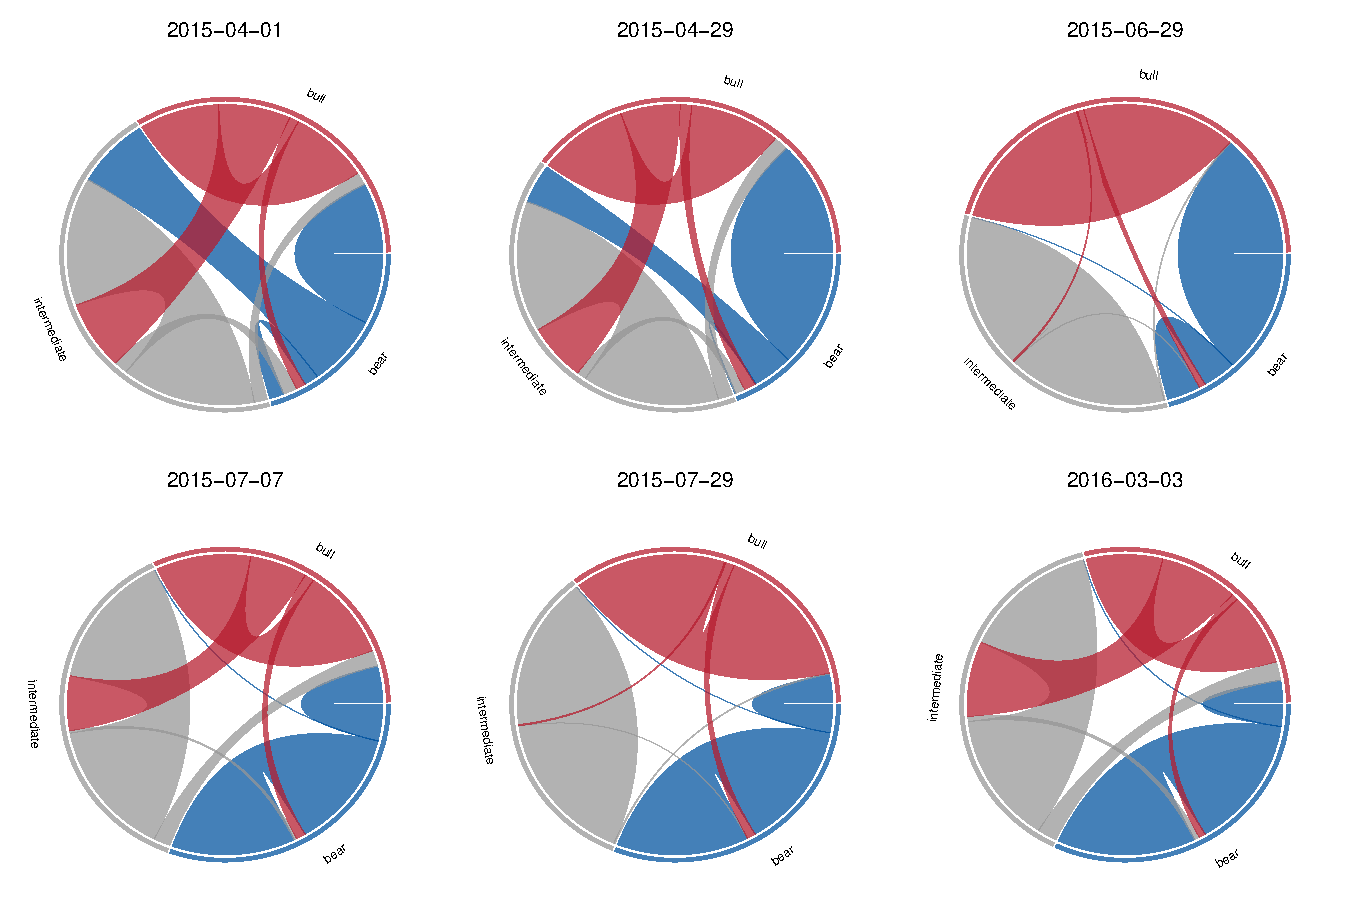
\includegraphics[width=\textwidth]{daily/transFig3.pdf}
        \caption{Typical state transition matrices during the entire period }
        \label{fig:CSI:transitiontypical}
        \end{figure}
To be more thorough, we also examine evolution of the state transition matrix
as the prediction processes, which leads to increases in data used to estimate parameters.
Illus.\,\ref{fig:CSI:transitionevo} plots the dynamic evolution of 
the matrix as size of in-sample data grows.
Dense fluctuations appear in June to July 2015, when the market has just passed its peak,
and in early this year, when another downturn took place.
It seems that falls of the market have greater impacts on the parameters than rises,
and that may be related to the long tail we mentioned in Sec.\,\ref{sec:positive:CSI:data}.

Illus.\,\ref{fig:CSI:transitiontypical} selects six chord diagrams within the entire observation period.
Market states tend to remain the same with more chance after the big fall and
hence the probability to transit into other states goes down,
that is, the market has a bigger tendency to behave like previous trading days.


\subsection{Conditional distribution parameters}
\label{sec:positive:CSI:distribution}
The estimation result of conditional distribution parameters for
CSI 300 in-sample is given as follow:
        \begin{equation}
        \left (
        \begin{array}{c c c}
        -1.66\%  &  0.13\%  &  2.13\%  \\
         1.02\%  &  0.99\%  &  1.23\%  \\
        \end{array}
        \right ).
        \end{equation}
Columns stand for states, the first row for expectation and the second for standard deviation.
The pattern resembles the one in \ref{sec:positive:SP:distribution} and clearly makes sense.


        \begin{figure}[!hbt]
        \center
        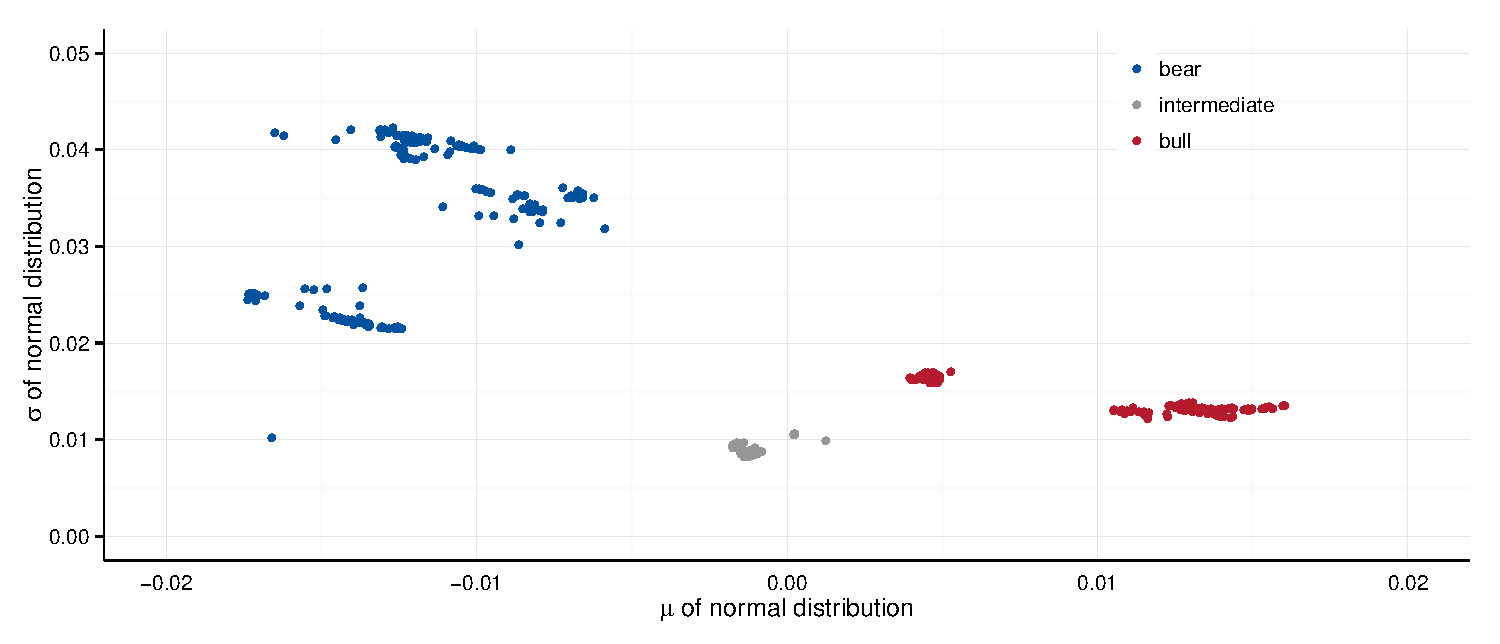
\includegraphics[width=\textwidth]{daily/paramFig1.pdf}
        \caption{Conditional distribution parameters across time}
        \label{fig:CSI:distscatter}
        \end{figure}

        \begin{figure}[!hbt]
        \center
        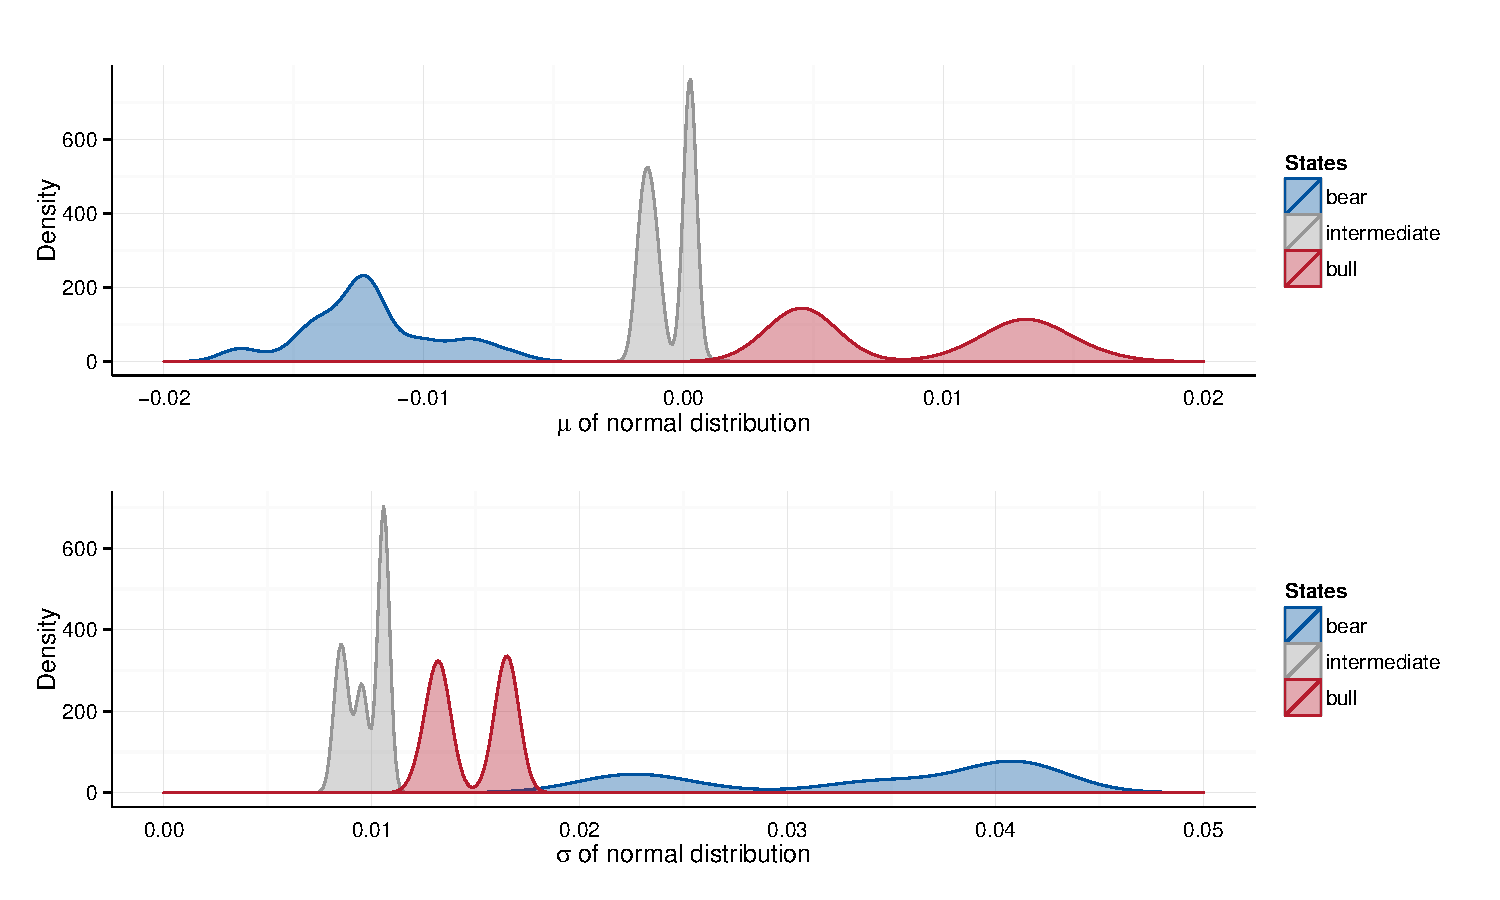
\includegraphics[width=\textwidth]{daily/paramFig2.pdf}
        \caption{Density distribution of conditional distribution parameters}
        \label{fig:CSI:distdist}
        \end{figure}
Illus.\,\ref{fig:CSI:distscatter} and \ref{fig:CSI:distdist} give 
the time-variation of distribution parameters.
High volatility of bears seems more significant than S\&P 500 case, 
but standard deviations are dispersed, 
which is reflected as flatness of the blue line in the downer part of Illus.\,\ref{fig:CSI:distdist}.
Multi-modality exists, indicating changes of the states and 
a potential need to increase the number of hidden states in the model.


\subsection{Global decoding and hidden states}
\label{sec:positive:CSI:states}

        \begin{figure}[!hbt]
        \center
        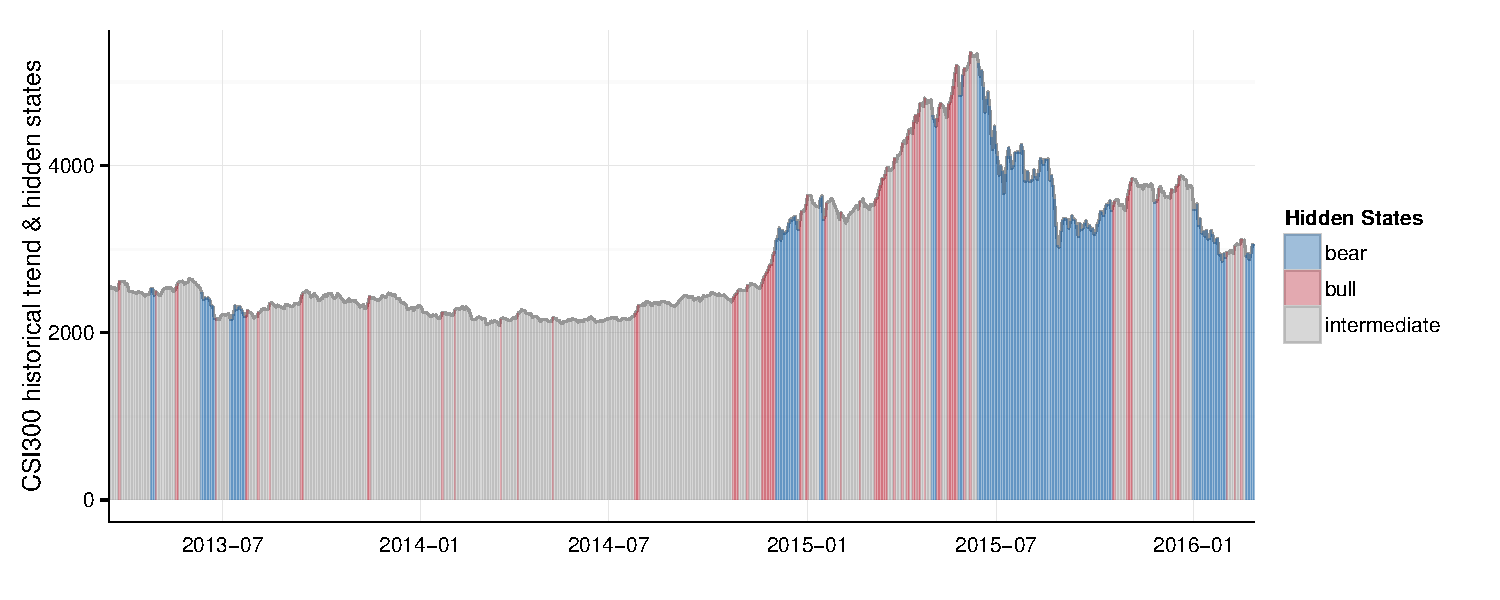
\includegraphics[width=\textwidth]{daily/statesFig1.pdf}
        \caption{CSI 300 in-sample trend and states sequence}
        \label{fig:CSI:seqstates}
        \end{figure}
Global decoding result meets our expectation well.
The intermediate state lasts for almost two years,
followed by frequent occurences of bulls.
Then there came the large bear until the rebounce,
and then the bear hit the market again.

        \begin{figure}[!hbt]
        \center
        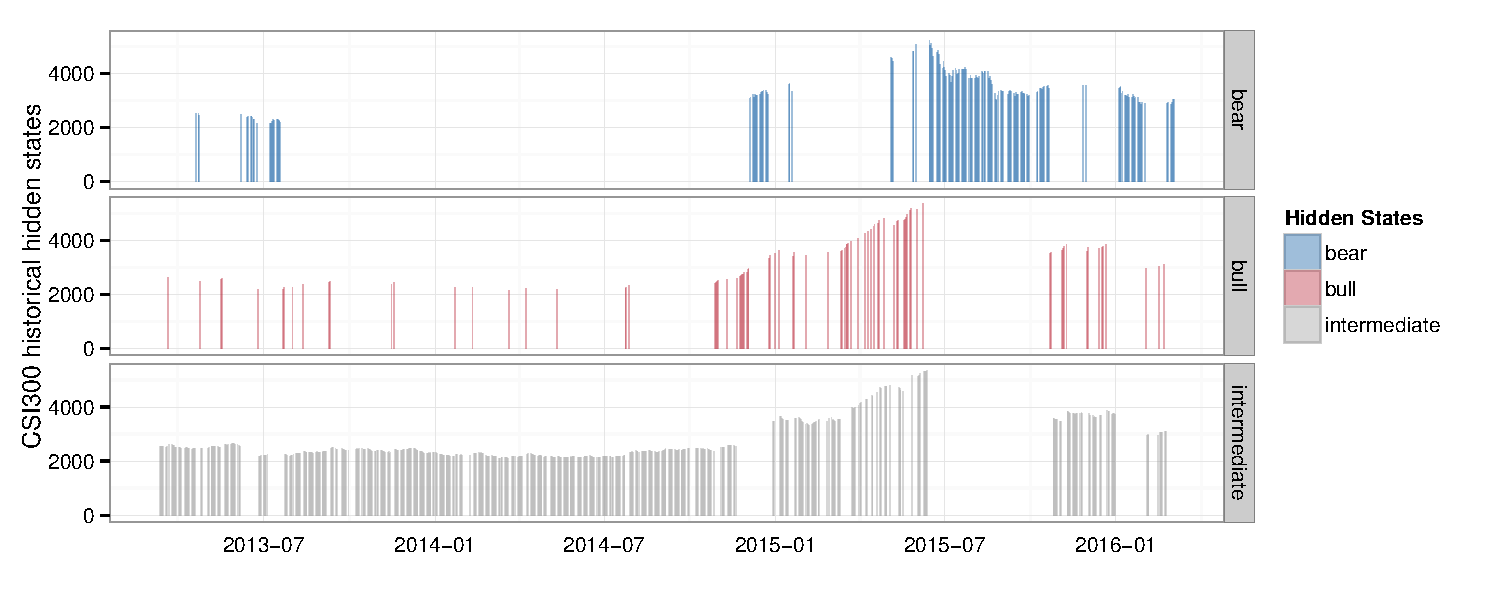
\includegraphics[width=\textwidth]{daily/statesFig2.pdf}
        \caption{CSI 300 historical hidden states}
        \label{fig:CSI:states}
        \end{figure}
The bull states have not appeared consecutively like the bear.
We suppose that is because when the market went up,
the returns were relatively small, 
and small positive returns accumulated to form a long-term bull with help of time,
while the bear came with large negative returns and conquered the market rapidly.
Results visualizations are presented in 
Illus.\,\ref{fig:CSI:seqstates} and \ref{fig:CSI:states}.

        \begin{figure}[!hbt]
        \center
        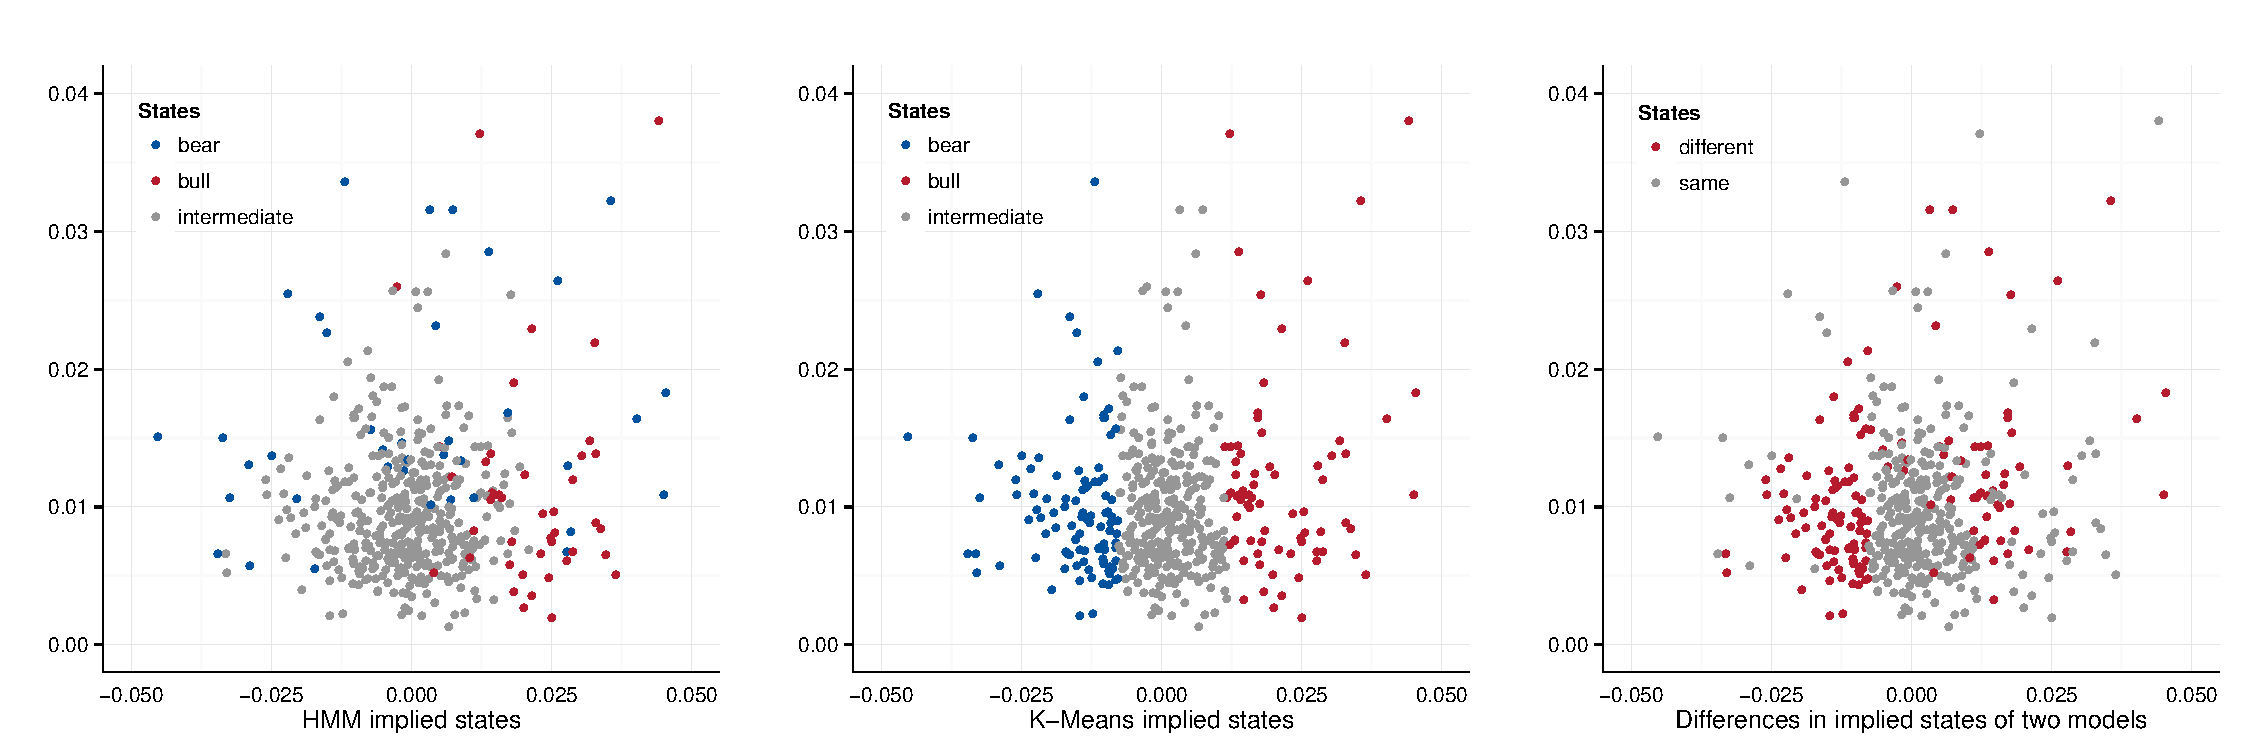
\includegraphics[width=\textwidth]{daily/statesFig3.pdf}
        \caption{Comparison between K-Means states and HMM hidden states}
        \label{fig:CSI:diffstates}
        \end{figure}
Similarly, differences between HMM states and K-Means states are examined 
(see Illus.\,\ref{fig:CSI:diffstates}).
Differences occur mainly in the bear zone, some in the bull, and few in the intermediate.
The pattern resembles one in Sec.\,\ref{sec:positive:SP:states} and 
we no longer repeat it here.


\subsection{Simulated prediction results}
\label{sec:positive:CSI:prediction}

        \begin{figure}[!hbt]
        \center
        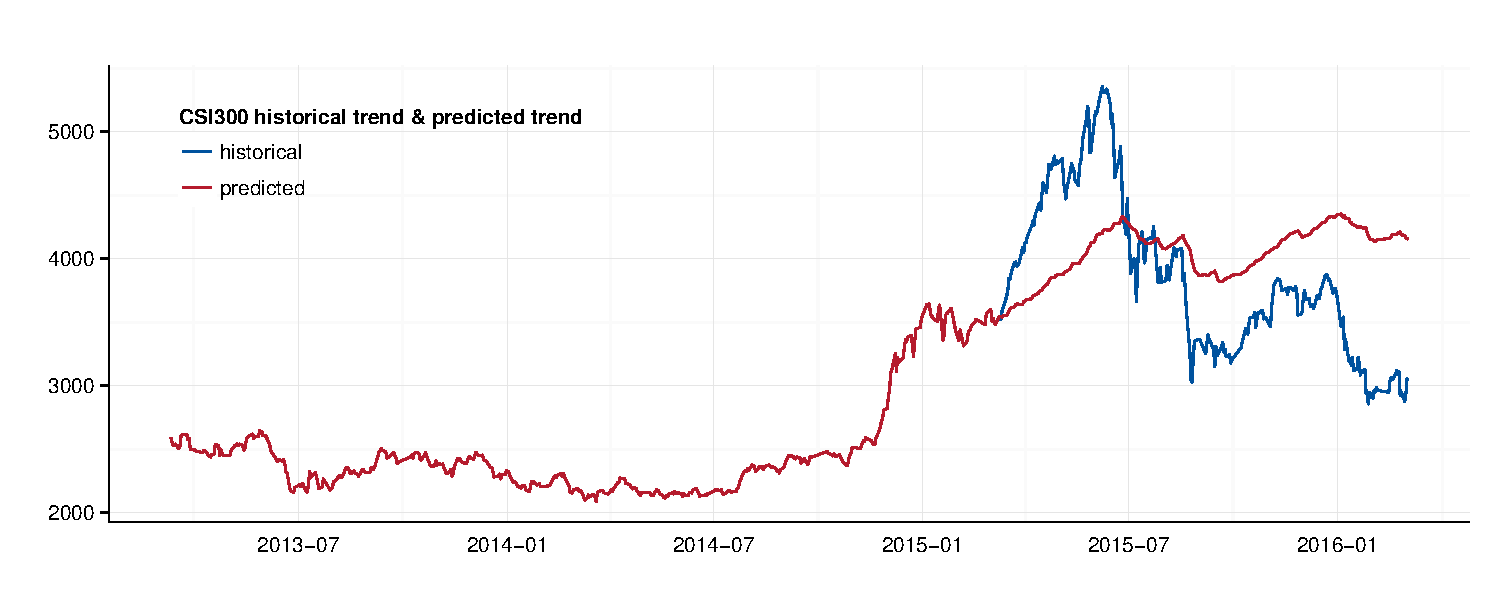
\includegraphics[width=\textwidth]{daily/predictionFig1.pdf}
        \caption{CSI 300 simulated prediction result}
        \label{fig:CSI:predictionall}
        \end{figure}
Simulated prediction result along with CSI 300 in-sample data
is plotted in Illus.\,\ref{fig:CSI:predictionall}.
The out-of-sample part is separatedly presented with daily return bars
in Illus.\,\ref{fig:CSI:predictionout}

        \begin{figure}[!hbt]
        \center
        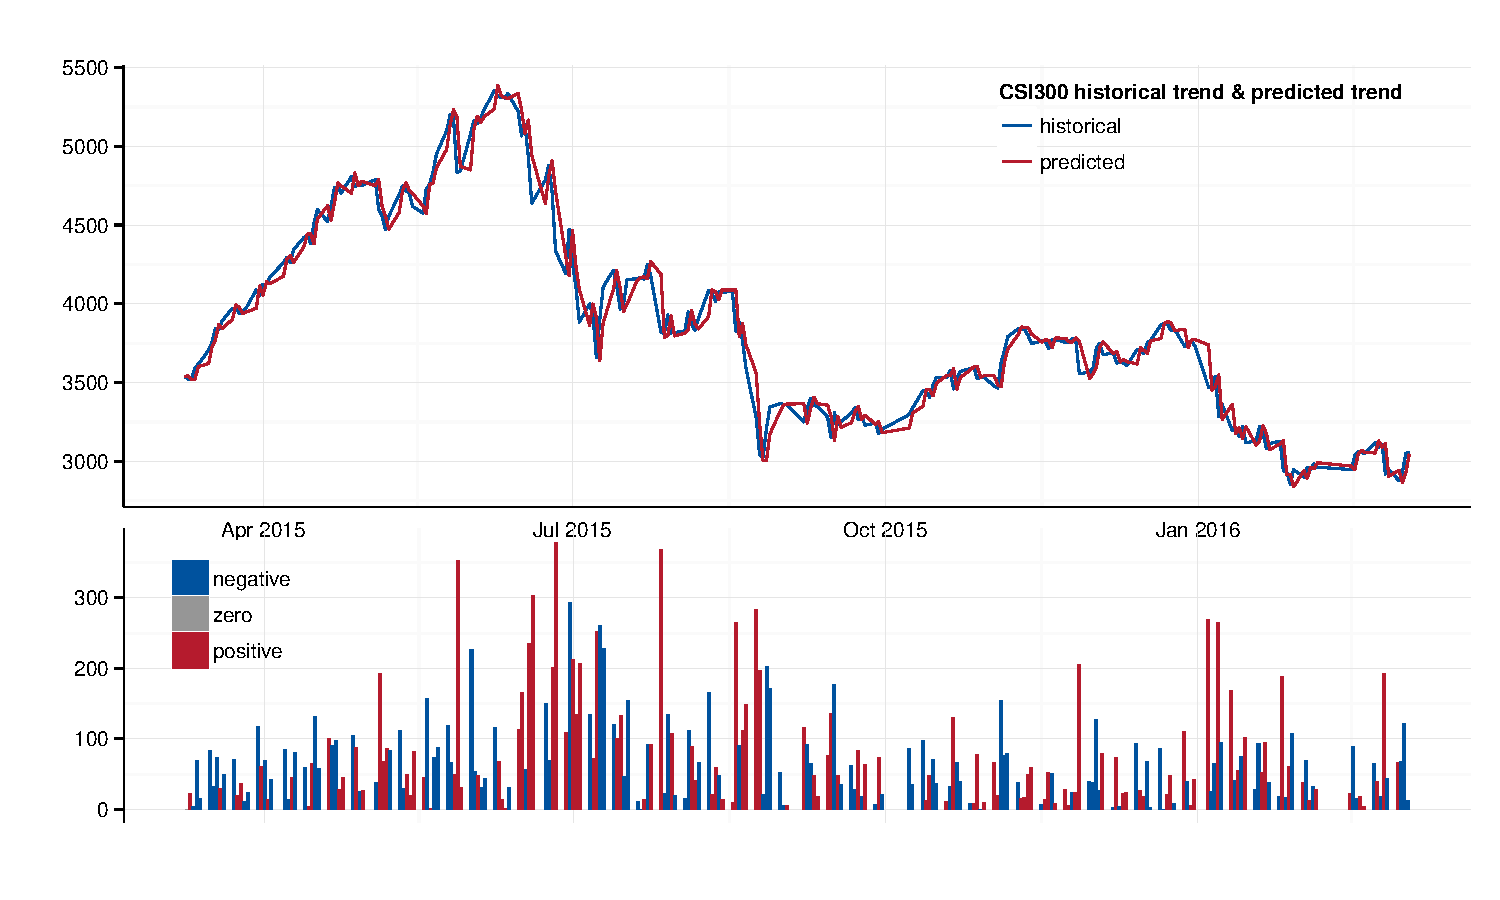
\includegraphics[width=\textwidth]{daily/predictionFig4.pdf}
        \caption{CSI 300 simulated prediction result out-of-sample part}
        \label{fig:CSI:predictionout}
        \end{figure}
The win ratio of the prediction is $50.2\%$, almost the same as in S\&P case,
and the extension and lagging pattern is more clearly conveyed.
At the very first of the out-of-sample period, 
the predicted index remains going up straight but with a lower slope,
which extends the trend before and also influenced by recent adjustments.
Downturn appears after the real fall takes place and the lag is quite obvious.
Prediction behaviors are similar in the rest part.
Confidence bands and adaptive prediction results are also visualized and 
the formats are similar as in S\&P case.
In order to avoid unnecessary information, 
we do not present the illustrations here and they will be listed in 
Appendix \ref{app:fig} in case the reader is interested
\footnote{Similar prediction and analysis are also carried out for 
CSI 300 data with medium frequencies 
(see Sec.\,\ref{sec:positive:CSI60} and Sec.\,\ref{sec:positive:CSI10},
and the figures are also presented in Appendix \ref{app:fig})}.

However, results are quite good for adaptive predictions.
Though the time lag effect still exists, 
it eliminates the error accumulation on the absolute level of the index.

%%%%%%%%%%%%%%%%%%%%%%%%%%

\section{Chinese CSI 300 Index medium frequency (60min) return series}
\label{sec:positive:CSI60}
CSI 300 medium frequency (60min) return data are selected within 
the same observation period as before.
The only difference is the observation frequency.
Higher frequency indicates that the number of data increase during the same period,
so we split the entire period into three parts,
each has length of about one year (from March to March).


\subsection{Global decoding and hidden states}
\label{sec:positive:CSI60:states}
        \begin{figure}[!hbt]
        \begin{center}
        \subfigure[Mar. 2013 $\sim$ Mar. 2014]
            {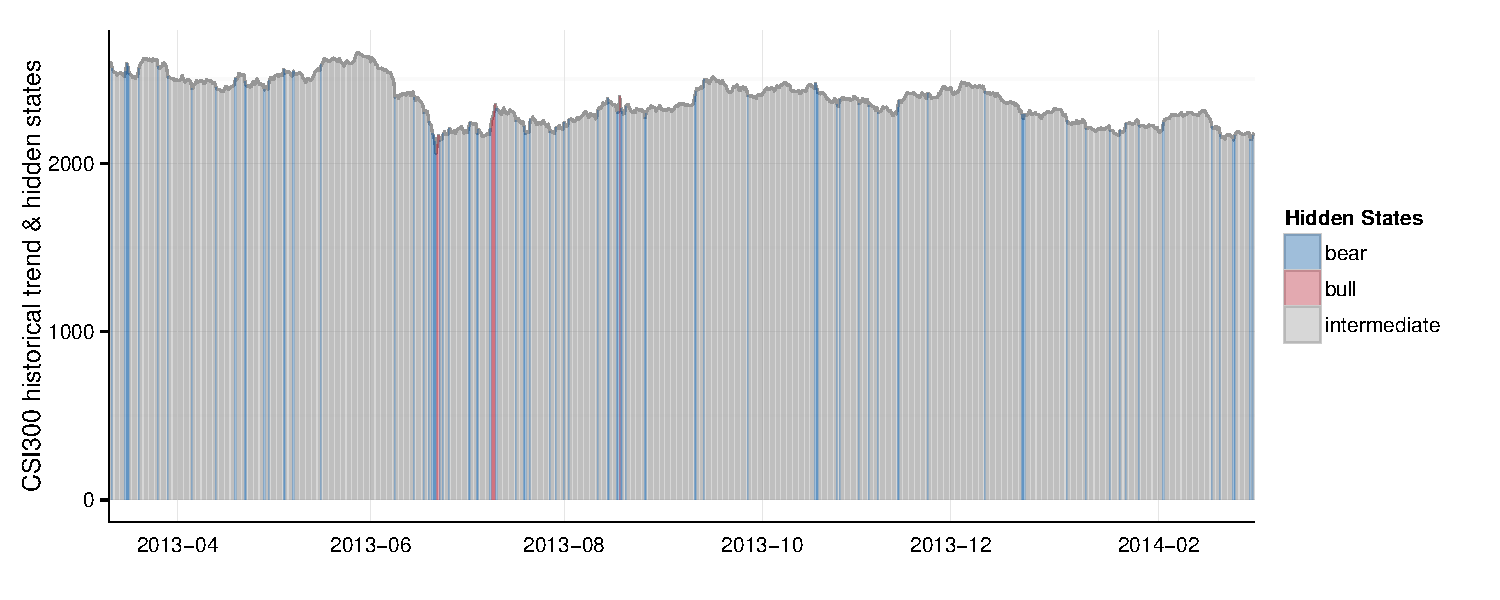
\includegraphics[width=0.49\textwidth]{60min_1314/statesFig1.pdf}}
        \subfigure[Mar. 2014 $\sim$ Mar. 2015]
            {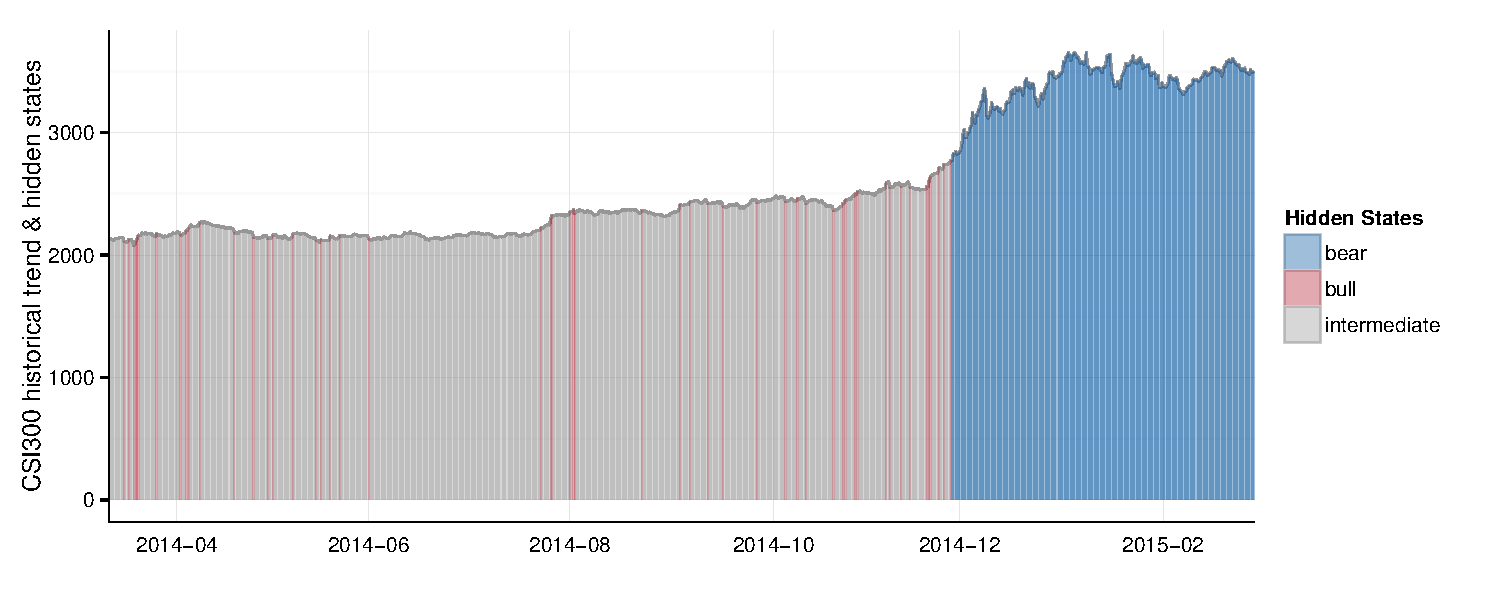
\includegraphics[width=0.49\textwidth]{60min_1415/statesFig1.pdf}}
        \end{center}
        \subfigure[Mar. 2015 $\sim$ Mar. 2016]
            {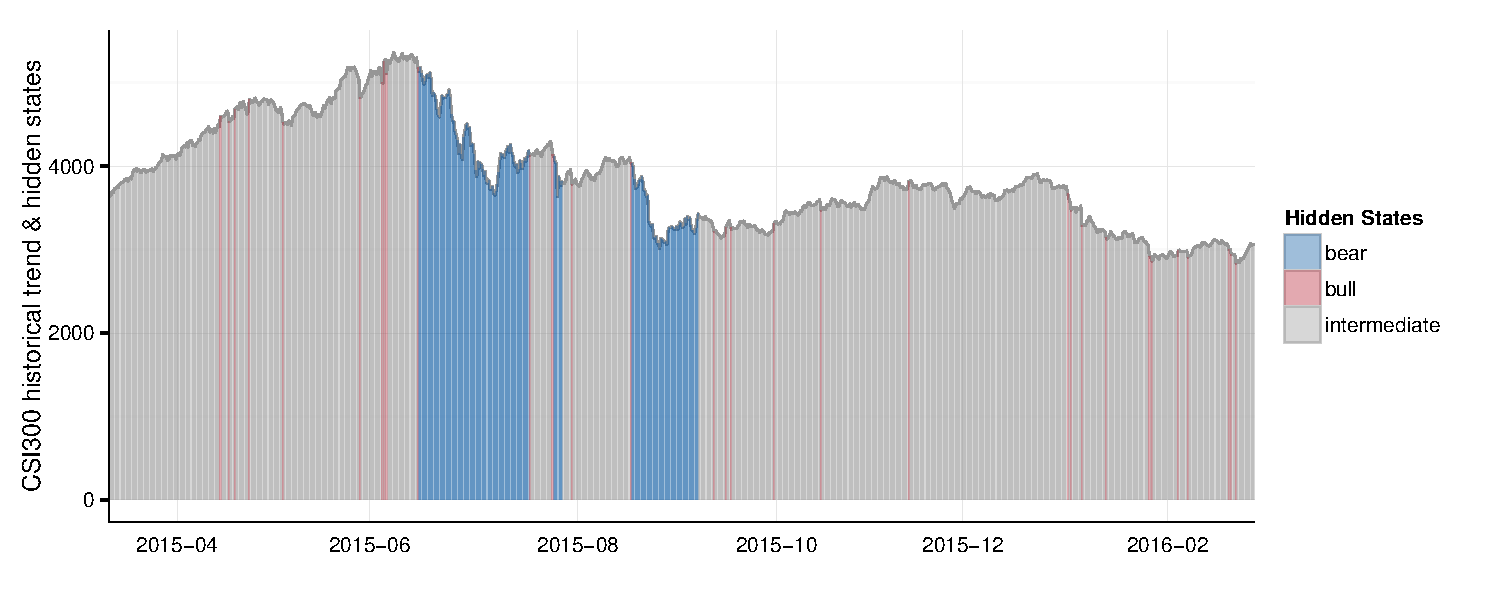
\includegraphics[width=0.49\textwidth]{60min_1516/statesFig1.pdf}}
        \caption{CSI 300 60min data global decoding results}
        \label{fig:CSI60:states}
        \end{figure}
Decoding results in year 2013 to 2014 matches our expectation,
while the result in the latter two sub-periods is quite astonishing.

The last part in Part (b) of Illus.\,\ref{fig:CSI60:states} presents 
the trend of a lasting rise but is identified as bear.
The conditional distribution parameters (60min basis
\footnote{The returns are calculated on a 60min basis and 
we do not annualize the data or change the scale to the same as former cases,
since compared to the actual value of the parameters,
we care more about their differences, orders and decoding and prediction results.}
) in the period are
        \begin{equation}
        \left (
        \begin{array}{c c c}
        0.108\%  &  0.019\%  &  0.115\%  \\
        1.207\%  &  0.324\%  &  0.827\%  \\
        \end{array}
        \right ).
        \end{equation}
The parameter pair corresponding to bear states has a positive expectation
and a relatively big standard deviation.
Thus, the ``bear'' state here has actually a higher expected return than the
intermediate state and is classified as bear because its volatility is higher
and expected return is lower than the bull.

As we mentioned before, 
the name of states here are artificially given to the states based on customs.
During Mar. 2014 to Mar. 2015, 
the market is at a (conventionally acknowledges) bull state almost all the time
and does not actually have a bear state, if not consider the small rebounces.
Therefore, although the labels do not meet our expectations,
the actual distributions are not that unexpected.


\subsection{Simulated prediction results}
\label{sec:positive:CSI60:prediction}
        \begin{figure}[!hbt]
        \begin{center}
        \subfigure[Mar. 2013 $\sim$ Mar. 2014]
            {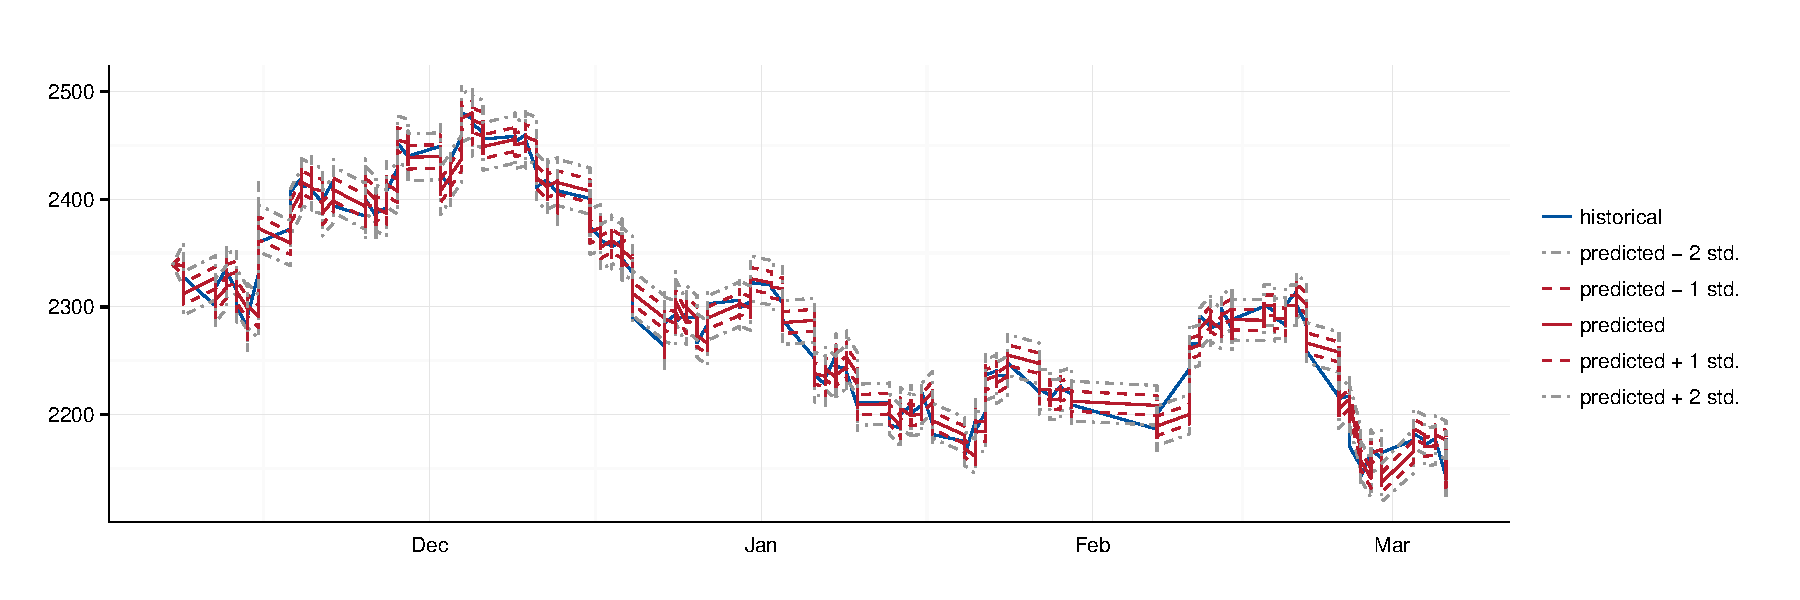
\includegraphics[width=0.49\textwidth]{60min_1314/predictionFig5.pdf}}
        \subfigure[Mar. 2014 $\sim$ Mar. 2015]
            {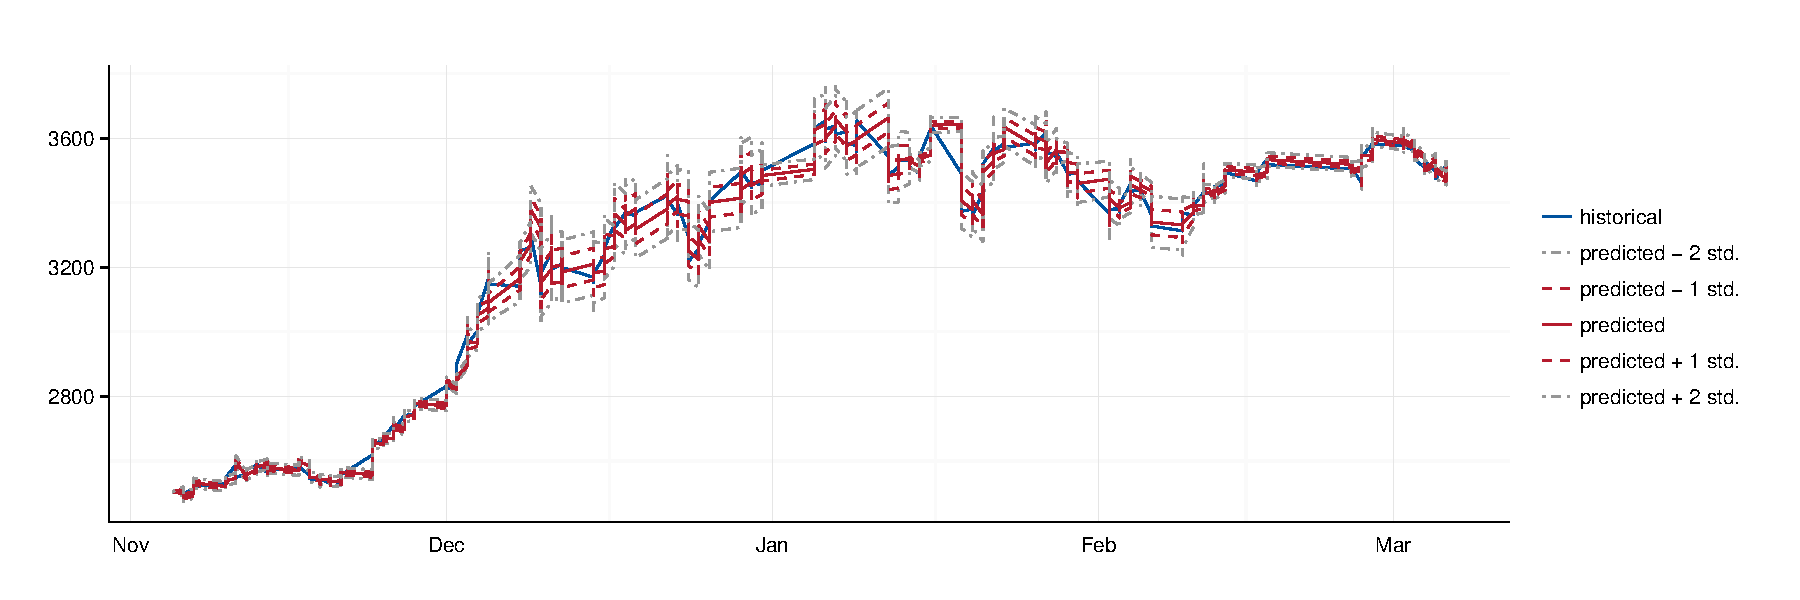
\includegraphics[width=0.49\textwidth]{60min_1415/predictionFig5.pdf}}
        \end{center}
        \subfigure[Mar. 2015 $\sim$ Mar. 2016]
            {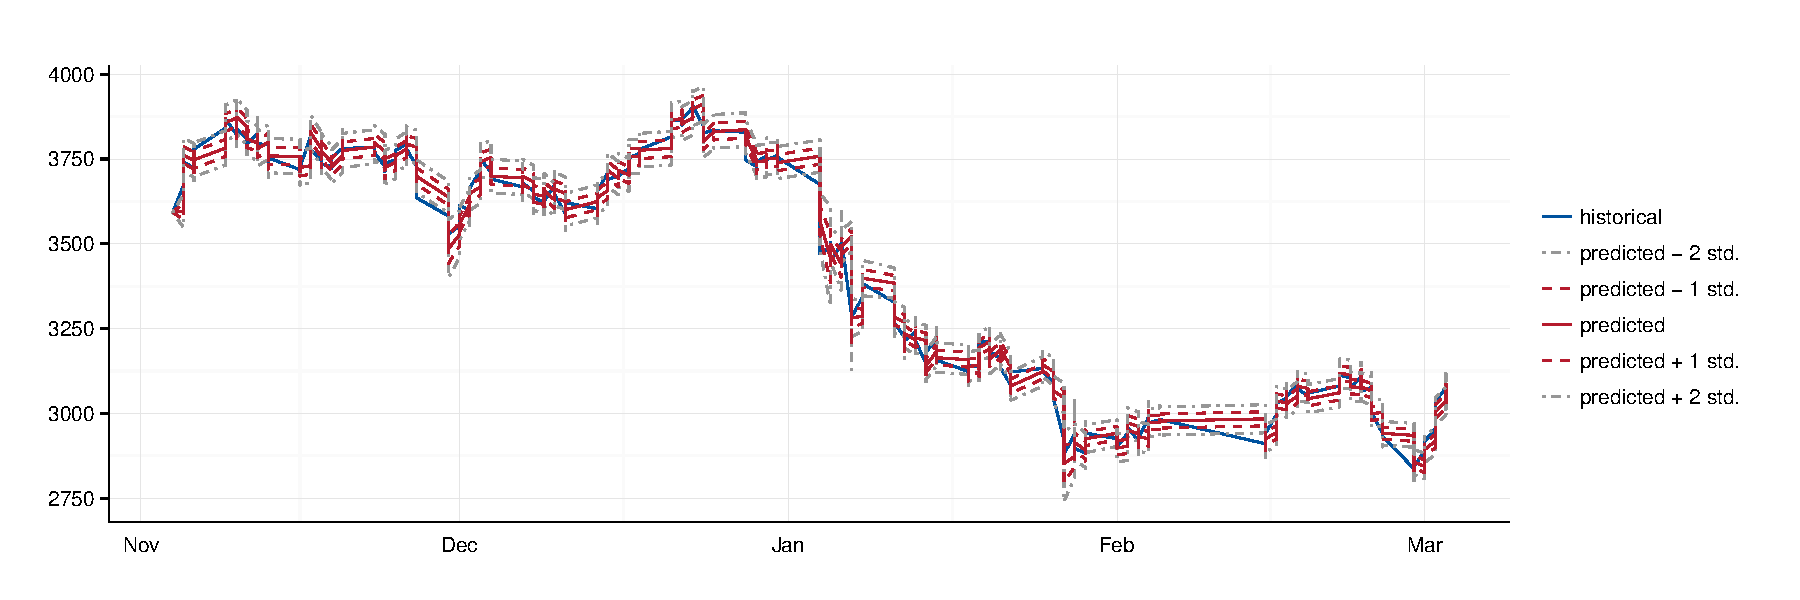
\includegraphics[width=0.49\textwidth]{60min_1516/predictionFig5.pdf}}
        \caption{CSI 300 60min data simulated prediction results}
        \label{fig:CSI60:prediction}
        \end{figure}
Win ratios in the three year are $51.7\%$, $55.5\%$ and $50.5\%$ separately,
which are all better than former cases.
Time lag effects and error accumulations exist for long-term prediction.
Adaptive prediction results are much better.

%%%%%%%%%%%%%%%%%%%%%%%%%%

\section{Chinese CSI 300 Index medium frequency (10min) return series}
\label{sec:positive:CSI10}
CSI 300 medium frequency (10min) return data have exactly the same structure as 60min data
except higher observation frequency.
This only difference enables us to examine the effect of observation frequency,
or data density within a given time period,
on the decoding results and prediction results.

\subsection{Global decoding and hidden states}
\label{sec:positive:CSI10:states}
        \begin{figure}[!hbt]
        \begin{center}
        \subfigure[Mar. 2013 $\sim$ Mar. 2014]
            {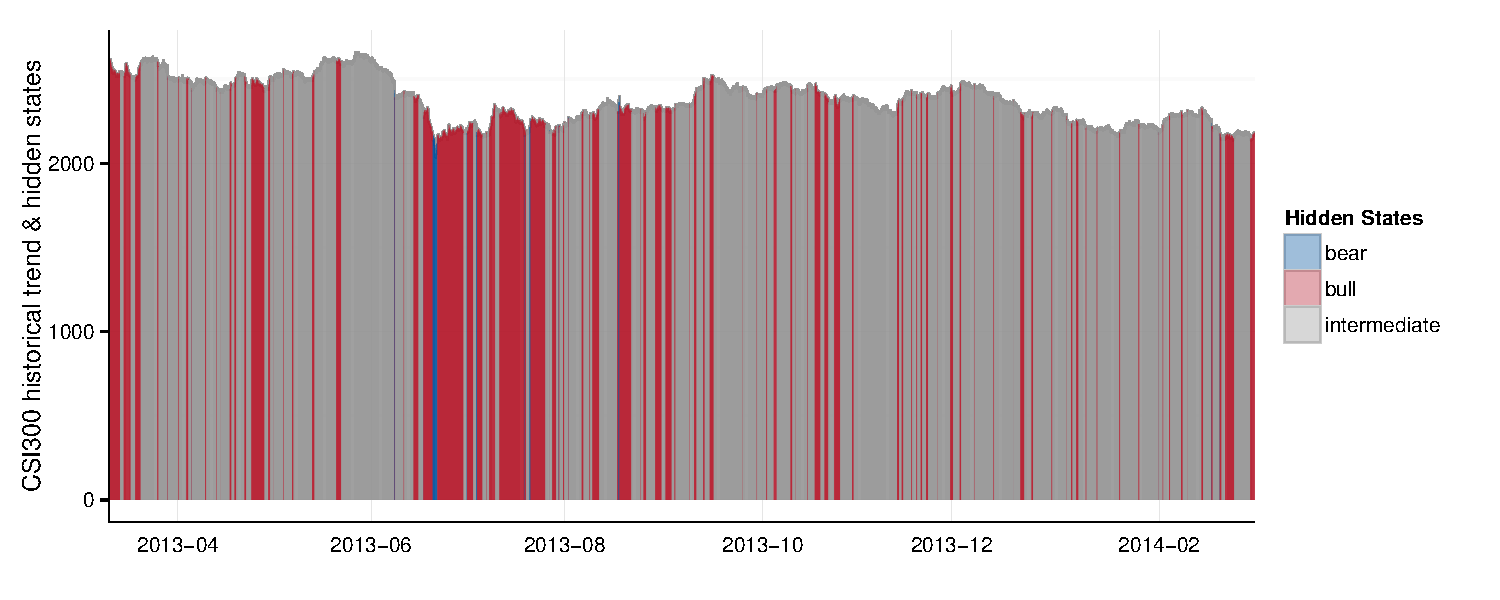
\includegraphics[width=0.49\textwidth]{10min_1314/statesFig1.pdf}}
        \subfigure[Mar. 2014 $\sim$ Mar. 2015]
            {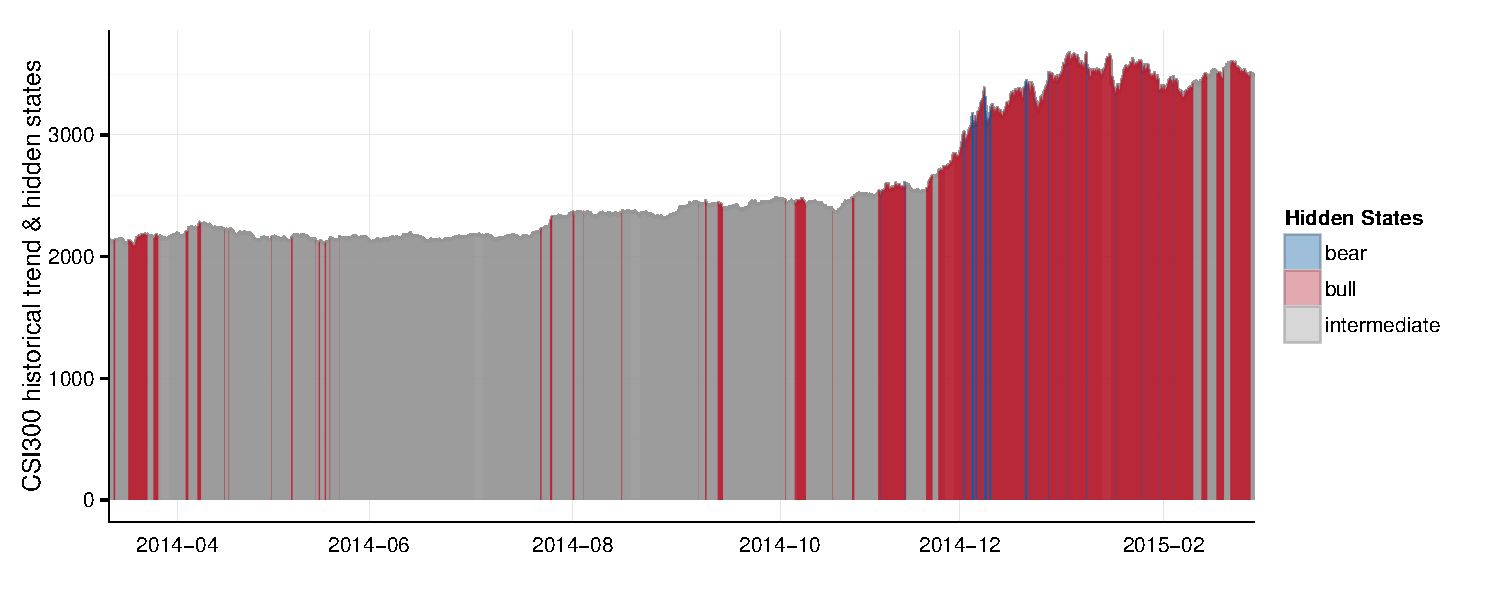
\includegraphics[width=0.49\textwidth]{10min_1415/statesFig1.pdf}}
        \end{center}
        \subfigure[Mar. 2015 $\sim$ Mar. 2016]
            {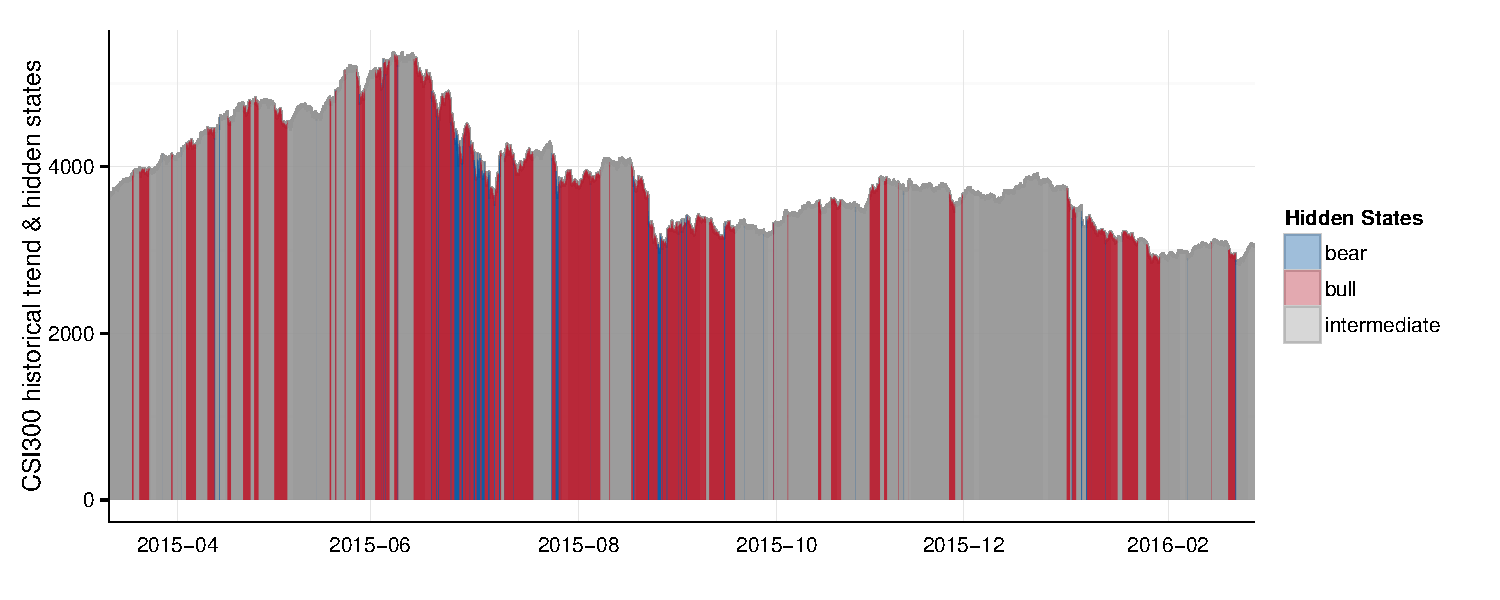
\includegraphics[width=0.49\textwidth]{10min_1516/statesFig1.pdf}}
        \caption{CSI 300 10min data global decoding results}
        \label{fig:CSI10:states}
        \end{figure}
Anomaly in 10min case occurs in year 2015 to 2016 (instead of 2014 to 2015 in 60min case).
Conditional distribution parameters (10min basis) are
        \begin{equation}
        \left (
        \begin{array}{c c c}
        -0.117\%  &  0.026\%  &  -0.031\%  \\
         1.627\%  &  0.269\%  &   0.515\%  \\
        \end{array}
        \right ).
        \end{equation}
So it is actually very similar to the 60min case,
just that the ``bull'' has a negative expected return and higher volatility here
while the anomaly in 60min case is related to the ``bear'' then.

\subsection{Simulated prediction results}
\label{sec:positive:CSI10:prediction}
        \begin{figure}[!hbt]
        \begin{center}
        \subfigure[Mar. 2013 $\sim$ Mar. 2014]
            {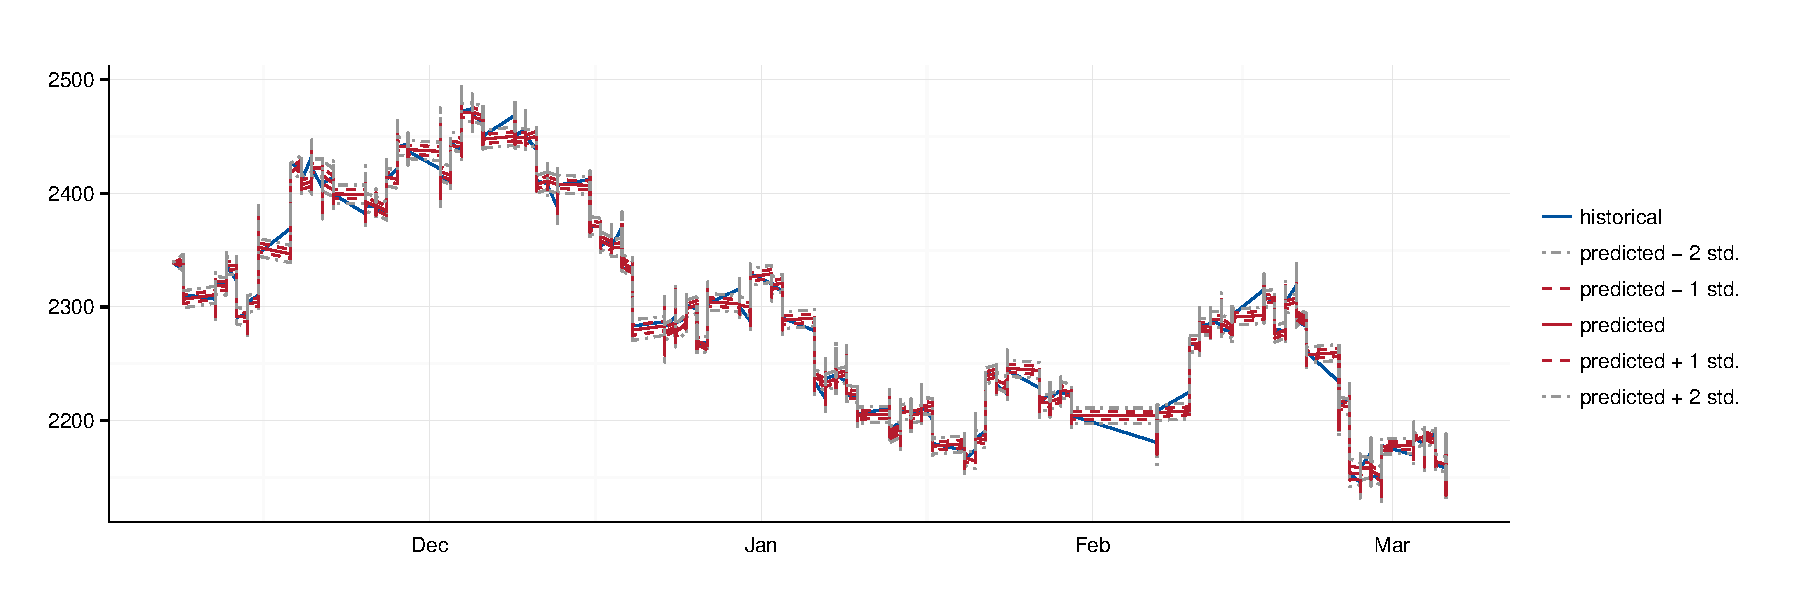
\includegraphics[width=0.49\textwidth]{10min_1314/predictionFig5.pdf}}
        \subfigure[Mar. 2014 $\sim$ Mar. 2015]
            {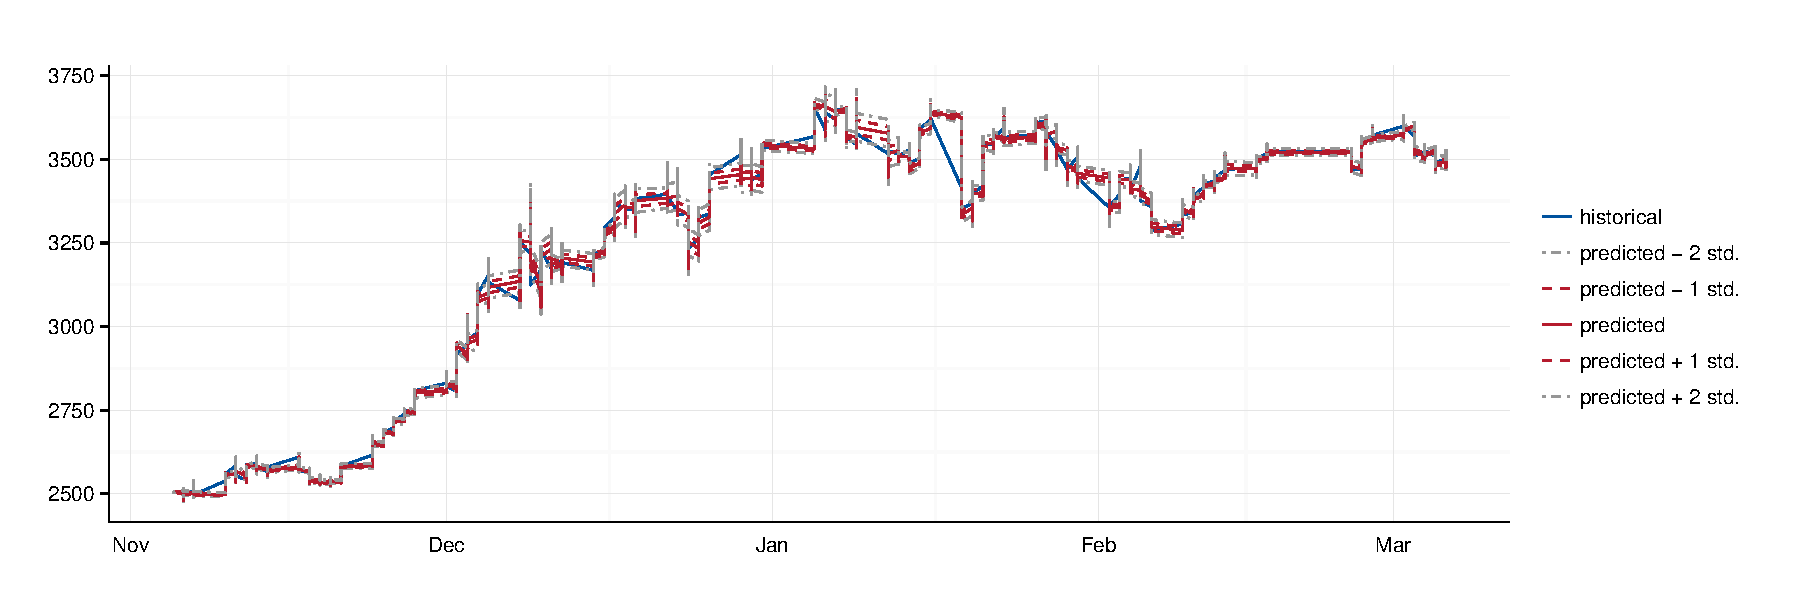
\includegraphics[width=0.49\textwidth]{10min_1415/predictionFig5.pdf}}
        \end{center}
        \subfigure[Mar. 2015 $\sim$ Mar. 2016]
            {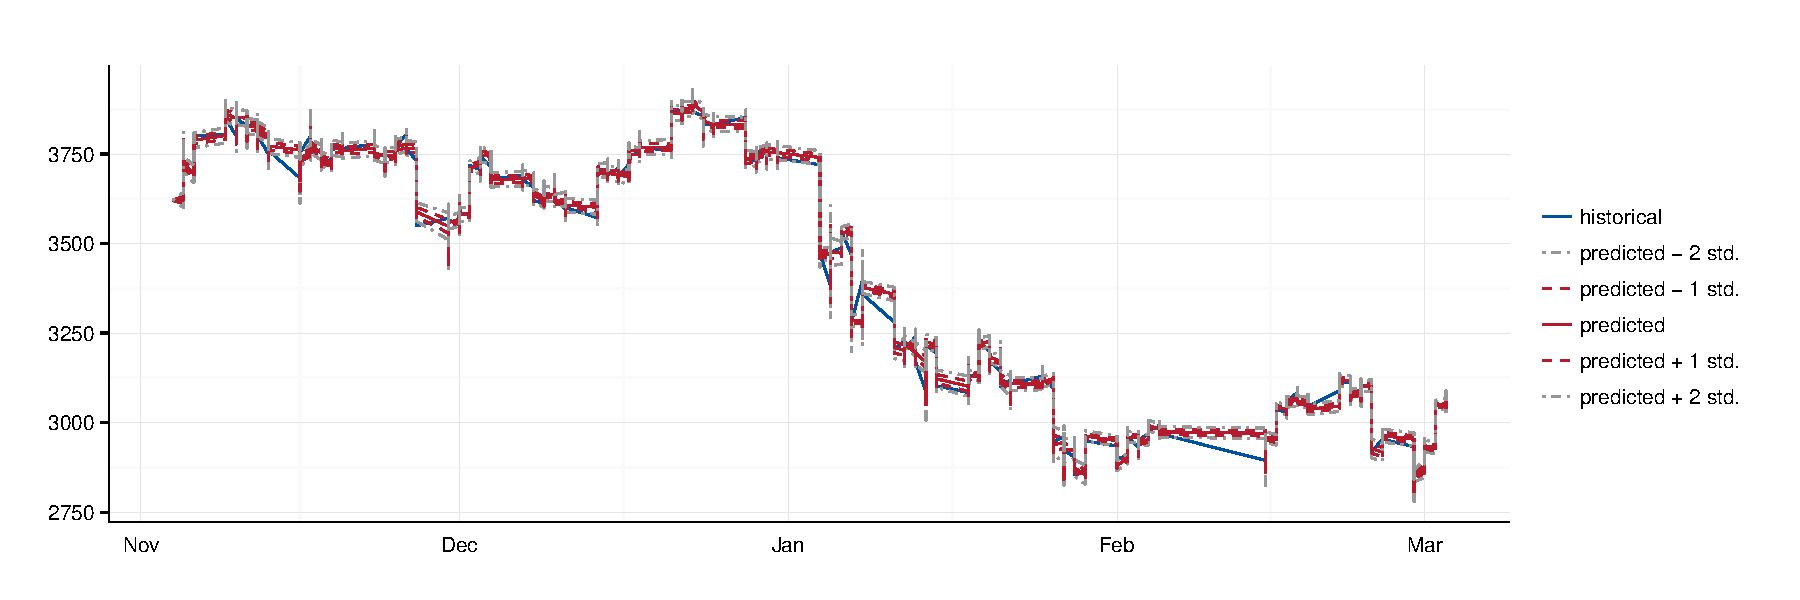
\includegraphics[width=0.49\textwidth]{10min_1516/predictionFig5.pdf}}
        \caption{CSI 300 10min data simulated prediction results}
        \label{fig:CSI10:prediction}
        \end{figure}
Win ratios in the three year are $51.7\%$, $57.5\%$ and $52.0\%$ separately,
better than ones in the 60min cases and of course the daily case.

Patterns are similar to 60min cases.
The slight increase in correctness is certainly not enough to 
cause revolutionary improvements of curve prediction and fitting,
yet still the increase is worth noticing and 
will be discussed about in Sec.\,\ref{sec:positive:result:frequency}.

%%%%%%%%%%%%%%%%%%%%%%%%%%

\section{Result analysis and comparisons}
\label{sec:positive:result}
Analysis of the results and various comparisons are carried out in this section.
Firstly we analyze all the prediction results and potential causes of errors.
Then comparisons from three different perspectives
(market, time period, data frequency) are conducted.
At last we discuss about setting of the number of hidden states,
as supplementary explanation to Assumption \ref{asp:states}. 

\subsection{Prediction correctness and error analysis}
\label{sec:positive:result:prediction}
So far we have performed eight complete stock return series predictions in total
(one for S\&P 500, seven for CSI 300 with different observation frequencies).
All results have a win ratio greater than $50\%$ (at least $50.2\%$),
so theoretically we can construct a trading strategy based on the model
and to profit through very frequent (not necessarily high-frequency) trades.
However, in practice, this ratio is quite low for real-life trading strategies 
since all kinds of transaction costs occur along with each trade, whatever win or lose.
Thus the prediction results heretofore has only theoretical values but 
not enough to apply to realistic problems.

As we found in previous sections, 
The biggest problem of the predictions is the time lag,
which proves Conjecture \ref{conj:lag} reasonable and very likely to be right.
Influences of outdated information is the main cause of prediction errors,
while this kind of errors can be reduced with sample reweighting or rolling window methods.
Potential methods to deal with time lags are presented in Sec.\,\ref{sec:future:lag} 
and no further discussions are given here.

Besides, the prediction method, given the current distribution of states, 
state transition matrix and corresponding conditional distribution parameters,
lower the correctness since it takes expectation (see Sec.\,\ref{sec:system:function:prediction}).
But it is statistically logical and meaningful, 
and reduces prediction variance for the next node.
We provide this point of view only to be thorough about potential causes of the errors.


\subsection{Comparisons between U.S. market and Chinese market}
\label{sec:positive:result:market}
Global decoding results and prediction correctness 
for both markets (daily data case) are similar.
There are not obvious contradictions to our expectation,
nor obvious differences in prediction effectiveness.
Thus currently it is safe to say that the performance of our model does not depend on the market.

However we should notice that the data we select have a very long length 
and they cover all (conventionally acknowledged) states that can be easily identified with our eyes.
One of the advantages of such data is that parameters distinguish clearly from one another.
Therefore, a more rigorous statement here is that,
when sample data are long enough to cover all traditional states 
(big rises, big falls, and long periods of fluctuations),
the model has no differences in performance for different markets.


\subsection{Comparisons among different time periods}
\label{sec:positive:result:time}
According to results in Sec.\,\ref{sec:positive:CSI60} and \ref{sec:positive:CSI10},
performances differ in terms of observation period.
Prediction correctness tends to increase during time when the trends are consistent,
e.g.\,bull all the time.
Actually this phenomenon seems overlap with Conjecture \ref{conj:lag} again, 
since inconsistency in trends actually means the ineffectiveness of old data.


\subsection{Comparisons among data of different frequencies}
\label{sec:positive:result:frequency}
Differences in performances with respect to data frequency are analyzed 
also based on Sec.\,\ref{sec:positive:CSI60} and \ref{sec:positive:CSI10}.
Prediction correctness in 10min cases are no smaller than in 60min cases 
($51.7\%$, $57.5\%$ and $52.0\%$ against $51.7\%$, $55.5\%$ and $50.5\%$).
Hence, apparently, higher observation frequency within the same period
leads to higher prediction accuracy,
since it contains more information with other conditions hold still.

        \begin{table}[!hbt]
        \center
        \caption{Brief description of all prediction results}
        \label{table:results}
        \begin{tabular}{c c c c c}
        \hline
        Target Index  &  Data Frequency  &  Time Period  &  Data Length  &  Win Ratio  \\
        \hline
        S\&P 500  &  daily  &  2013$\sim$2016  &  757  &  50.4\%  \\
        CSI 300   &  daily  &  2013$\sim$2016  &  729  &  50.2\%  \\
        CSI 300   &  60min  &  2013$\sim$2014  &  968  &  51.7\%  \\
        CSI 300   &  60min  &  2014$\sim$2015  &  976  &  55.5\%  \\
        CSI 300   &  60min  &  2015$\sim$2016  &  972  &  50.5\%  \\
        CSI 300   &  10min  &  2013$\sim$2014  &  5808  &  51.7\%  \\
        CSI 300   &  10min  &  2014$\sim$2015  &  5856  &  57.5\%  \\
        CSI 300   &  10min  &  2015$\sim$2016  &  5832  &  52.0\%  \\
        \hline
        \end{tabular}
        \end{table}
Table \ref{table:results} present a brief description of the eight groups 
on data frequency, time periods, data length (the number of records) and win ratios.

\subsection{Comparisons among different number of hidden states}
\label{sec:positive:result:states}
        \begin{figure}[!hbt]
        \begin{center}
        \subfigure[AIC vs. N]
            {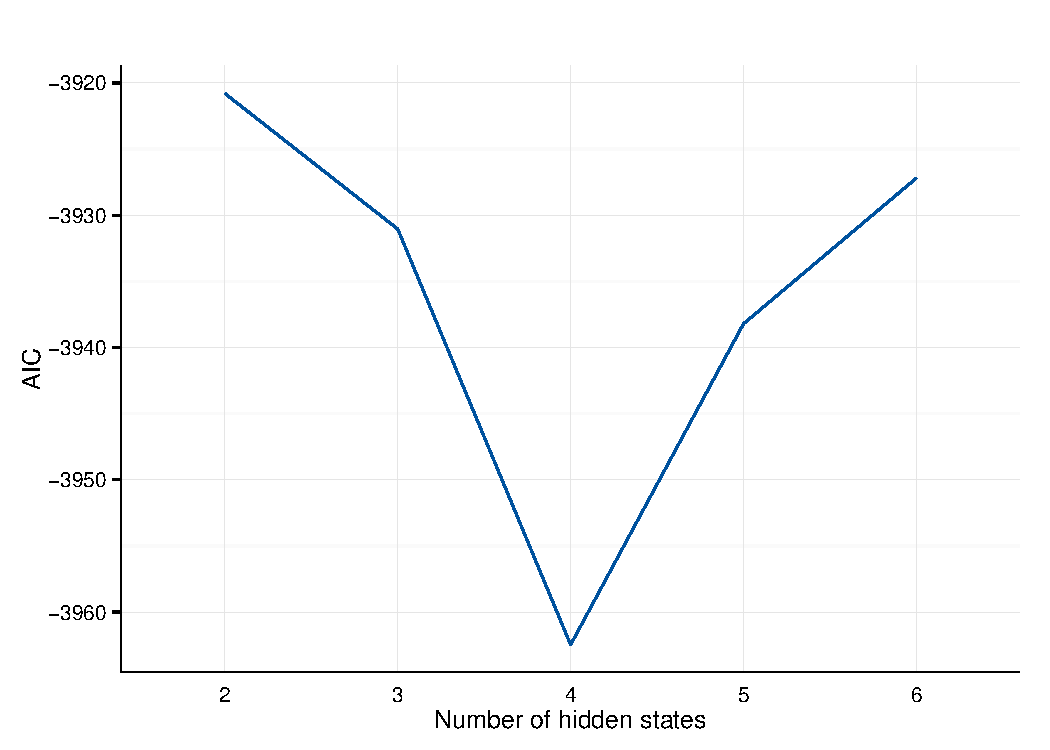
\includegraphics[width=0.45\textwidth]{states/numStateAIC.pdf}}
        \subfigure[BIC vs. N]
            {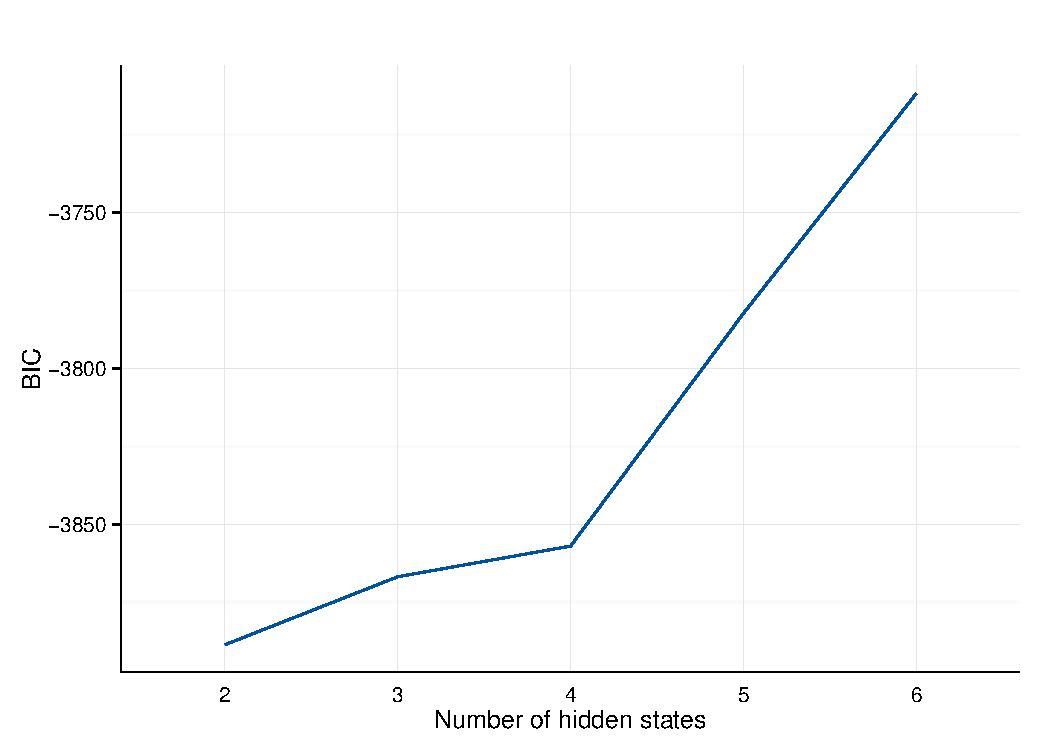
\includegraphics[width=0.45\textwidth]{states/numStateBIC.pdf}}
        \end{center}
        \caption{Goodness of fit for different number of hidden states}
        \label{fig:result:states}
        \end{figure}
We state in Assumption \ref{asp:states} that the markets have only three hidden states
and we name them as bear, intermediate and bull.
As is conventionally acknowledged, there are bull markets and bear markets.
However there are also intermediates that do not have obvious trends 
and fluctuations dominate during the period,
where only two states are not enough to describe the markets.
Certainly more market states could be introduced to the model 
(e.g.\,four to represent big rises, small rises, small falls and big falls),
but more states also bring higher risk of over-fitting and 
higher possibility to lack in realistic economic meanings.

Illus.\,\ref{fig:result:states} and Table \ref{table:result:states} indicate that 
two is the optimal parameter of 
the number of states based on BIC and four optimal according to AIC.
Thus we choose three as the parameter, 
which is the most widely used (see \cite{Zucchini:2009df,Dias:2015ky,Nystrup:2015ic}),
statistically (nearly) optimal and also economically meaningful.
Yet still the reader should notice that it is possible there are more optimal parameter selections.

        \begin{table}[!hbt]
        \center
        \caption{Numerical results of goodness of fit for different number of states}
        \label{table:result:states}
        \begin{tabular}{c c c}
        \hline
        Number of States  &  \hspace*{5em}AIC\hspace*{5em}  &  \hspace*{5em}BIC\hspace*{5em} \\
        \hline
        2   &   -3920.80    &   -3888.71    \\
        3   &   -3931.05    &   -3866.86    \\
        4   &   -3962.47    &   -3857.02    \\
        5   &   -3938.21    &   -3782.33    \\
        6   &   -3927.20    &   -3711.71    \\
        \hline
        \end{tabular}
        \end{table}


% !TEX encoding = UTF-8 Unicode
%%==================================================
%% thanks.tex for SJTU Bachelor Thesis
%% version: 0.5.2
%% Encoding: UTF-8
%%==================================================

\chapter{Conslusion}
\label{chap:conclusion}

In this chapter we summarize all contents above of this thesis and 
draw some conclusions on the stock return series prediction work we have done.

Up to now,
we have formally introduced the hidden Markov model (HMM) in Ch.\,\ref{chap:HMM},
including the model formulation and important statistics, 
model estimation methods, and ways to perform forecasts and decoding.
As a simple dynamic Bayesian network,
HMM is easy to be realized, 
and it excavates the information not only about the stock returns themselves 
but also the classifications of them.
which enables us to analyze the data from the angles of points and also intervals.
The number of model parameters in under control of the number of hidden states,
at the level of $\co(N^2)$ ($N$ represents the number of states),
which is usually small in empirical analysis.
From these perspectives, 
HMM is quite suitable to apply for stock return series analysis and prediction,
due to its easy implementation, appropriate complexity and small number of parameters.

In Ch.\,\ref{chap:system} we have constructed the stock return series prediction system,
which combines model initialization with K-Means,
model estimation, historical analysis (with HMM global decoding) and visualization.
The system is adaptive to different data populations 
(w.r.t.\,target index, time horizon, observation frequency, etc.) and 
exogenous parameters (e.g.\,the number of hidden states).
It is also complete, encapsulated and user-friendly 
(see Appendix \ref{app:code} for the user manuscript and source codes).

In Ch.\,\ref{chap:positive} we have carried out empirical analysis on 
both U.S. (the S\&P 500 Index) and Chinese (the CSI300 Index) stock markets.
With some modest assumptions,
the system has been well functioning for all the analysis.
From the perspective of prediction correctness,
the system is effective and always has a win ratio greater than 50\%,
and sometimes approaches 60\% under certain circumstances.
We can also draw the conclusion that data populations with higher observation frequencies
tend to outperform those with lower frequencies in this system
due to the difference in the amount of information contained in the data.
From the view of global decoding,
we come up to the conclusion that data populations with longer time horizon 
(i.e.\,longer observation period)
tend to have (better) global decoding results that more fit our usual acknowledgements.
Potential for improvement of the HMM-based system lies in 
the incorporation of resampling or sample reweighting,
which shall largely ameliorate the time lag effect.
This part will be briefly introduced in Ch.\,\ref{chap:future}.

To sum up,
we have successfully constructed the HMM-based stock return series prediction system
and have accomplished all the aims of this thesis.
We want to reinstate that this thesis in aimed to fulfill a complete implementation
of stock return prediction with HMM,
while we have no intention to realize the improvements of model-level techniques.
Finally note that the model is imperfect and there exist many unaddressed issues.
We cover some of them in the last chapter and hope to incorporate such improvements in future works.
% !TEX encoding = UTF-8 Unicode
%%==================================================
%% thanks.tex for SJTU Bachelor Thesis
%% version: 0.5.2
%% Encoding: UTF-8
%%==================================================

\chapter{Future work}
\label{chap:future}

In the final chapter, 
we briefly talk about some remaining issues mentioned in the previous chapters
and potential directions for future research.
In Sec.\,\ref{sec:future:lag} we discuss about the time lag effect that has been mentioned
multiple times in Ch.\,\ref{chap:positive},
and we propose some (possibly) feasible solutions to the problem.
In Sec.\,\ref{sec:future:PF} we introduce particle filters,
which is currently a preferred method for HMM estimations \cite{Jacob:2015um}.
We address these issues here merely for the reader's information,
and we hope to deal with them in future works.

%%%%%%%%%%%%%%%%%%%%%%%%%%

\section{Dealing with time lags}
\label{sec:future:lag}
As we stated in Conjecture \ref{conj:lag},
incorporation of too much out-dated information leads to large prediction errors,
and the results worsen as time goes by,
i.e.\,with the iterative (loops of out-of-sample data) predictions process.

The essential issue embedded in the problem is that all data sample take up equal weight
when they are used to fit the model.
The latest data point has the same significance as the one from a year ago,
which is intuitively problematic.
Therefore, reweighting of the sample observations are necessary to deal with the time lag effect.

We introduce two different ways in this section.
The first one described in Sec.\,\ref{sec:future:lag:rolling} implements a rolling window,
which makes cut-off of the data that are too old.
This method is mostly used in industries due to its simplicity and flexibility.
The second one presented in Sec.\,\ref{sec:future:lag:EWEM}, more popular in academia,
is the exponentially weighted EM algorithm.
The algorithm remains all sample data from the population,
and the only difference with the traditional EM is that the sample observations are reweighted.


\subsection{Prediction with rolling windows}
\label{sec:future:lag:rolling}
The rolling window method,
as is indicated from the name itself,
refers to the idea that the data sample (set) is updated with arrival of new observations
while the size of the sample remain the same.
Eq.\,\ref{eq:future:rolling} shows the dynamic process of data set changing.
		\begin{equation}
		\label{eq:future:rolling}
		\dots,\rlap{$\underbrace{\phantom{x_{t-l+1},x_{t-l+2},\dots,x_{t-1},x_{t}}}_{\text{sample}_{t}}$}
		x_{t-l+1},\overbrace{x_{t-l+2},\dots,x_{t-1},x_{t},x_{t+1}}^{\text{sample}_{t+1}},\dots
		\end{equation}

Every time when the system processes to the next loop,
the first (in time) sample point is discarded and the newly come observation is included,
and the length of observation series used to fit model remains $l$.
Simply put, we cut the tail of the data sample whenever a new observation is made.
Essentially the rolling window is a reweighting method,
only the weight for all out-dated observations are arbitrarily zero
and ones remained in the sample are equally weighted.

Due to its easiness to implement,
the rolling window method is commonly used in real-world financial analysis.
The only changeable parameter in the method is the size of the sample.
Usually the parameter is chosen to have some realistic meanings,
e.g.\,for analysis on daily return data,
$l$ is usually chosen as $5,10,21,63$, 
which separately stands for a week, half-month, a month and three months,
counting in trading days.
Optimization within the small pool helps us to find a (relatively) good choice of the parameter,
meanwhile reduces the risk of over-fitting.


\subsection{Exponentially weighted EM algorithm}
\label{sec:future:lag:EWEM}
Considering the change of importance over the time,
a few weighting methods are created based on the moving average (MA) concept.
The methods are then adopted beyond MA and used along with many other techniques,
e.g.\,the EM algorithm.

The exponentially weighted expectation maximization (EWEM) algorithm,
inspired by the idea of exponentially weighted moving average (EWMA),
performs reweighting of the sample observations.

Recall Eq.\,\ref{eq:HMM:EM:CDLL} and we rewrite the iteratively maximization problem
in form of function of the parameter $\btheta$:
		\begin{equation}
		\label{eq:future:CDLL}
		Q(\btheta,\btheta^{(i-1)}) = E \left[ \log p(\bx,\bs \mid \btheta)
			\mid \bx,\btheta^{(i-1)} \right],
		\end{equation}
and we shall introduce a time-dependent weight $\eta$ into Eq.\,\ref{eq:future:CDLL}:
		\begin{equation}
		\label{eq:future:CDLL:time}
		\begin{aligned}
		\hat{Q}(\btheta,\btheta^{(i-1)}) & = E\left[\log\eta p(\bx,\bs \mid \btheta) 
			\mid \bx,\btheta^{(i-1)} \right] \\
		& = E\left[\eta\log p(\bx,\bs \mid \btheta) \mid \bx,\btheta^{(i-1)} \right] \\
		& = \sum_{s \in \hs}\eta\log p(\bx,s \mid \btheta) p(s \mid \bx,\btheta^{(i-1)})
		\end{aligned}
		\end{equation}

The full description and analysis of the method 
(including definition, implementation, convergence result, etc.)
is explained in details in \cite{Zhang:2005tp},
and we do not provide further steps here.
The two equations above are enough for the introduction to the general idea.

The EWEM algorithm is more complex than the rolling window method and 
much more difficult to add to the traditional EM algorithm,
thus it is mostly discussed about in academia while seldom implemented for industrial research.
Yet the idea is very enlightening and 
we hope to study further on the sample reweighting of HMM in the future.

%%%%%%%%%%%%%%%%%%%%%%%%%%

\section{Particle filters}
\label{sec:future:PF}
Particle filters (PF) are also known as sequential Monte Carlo (SMC) methods,
which is a set of genetic-type particle Monte Carlo methodologies 
to solve the filtering problem \cite{wiki:PF},
and is firstly proposed in \cite{DelMoral:1997dp, Liu:1998fp}.

Firstly we re-formulate the HMM problem in a uniform way:
		\begin{subequations}
		\begin{align}
		\bx_n & = m_n(\bs_n,\epsilon_n), \\
		\bs_n & = h_n(\bs_{n-1},\eta_n),
		\end{align}
		\end{subequations}
where $\bx$ is the observed variable (vector) and $\bs$ the state variable (vector).
In previous chapters,
we redeem that both $\bs$ and $\bx$ are discrete and $\bs$ is even categorical,
while they may be continuous, discrete or even combined of the two \cite{Creal:2012ct}.
The functions $m_n$ and $h_n$ are very likely to be nonlinear and with unknown forms.

Similar to before, we write some important statistics as follows:
		\begin{itemize}
		\item joint smoothing distribution
			\begin{equation}
			\label{eq:PF:smoothing}
			p(\bs_{0:n} \mid \bx_{1:n};\theta) = \frac{p(\bs_{0:n},\bx_{1:n};\theta)}{p(\bx_{1:n};\theta)};
			\end{equation}
		\item transition density
			\begin{equation}
			\label{eq:PF:transition}
			p(\bs_n \mid \bx_{1:n-1};\theta) = \int p(\bs_n \mid \bs_{n-1};\theta)
				p(\bs_{n-1} \mid \bx_{1:n-1};\theta)\ d\bs_{n-1};
			\end{equation}
		\item filtering distribution
			\begin{equation}
			\label{eq:PF:filtering}
			\begin{aligned}
			p(\bs_n \mid \bx_{1:n};\theta) & = 
				\frac{p(\bx_n,\bs_n \mid \bx_{1:n-1};\theta)}{p(\bx_n \mid \bx_{1:n-1};\theta)} \\
			& = \frac{p(\bx_n \mid \bs_n;\theta)p(\bs_n \mid \bx_{1:n-1};\theta)}
				{\int p(\bx_n \mid \bs_n;\theta)p(\bs_n \mid \bx_{1:n-1};\theta)\ d\bx_n};
			\end{aligned}
			\end{equation}
		\item forecast distribution
			\begin{equation}
			\label{eq:PF:forecast}
			p(\bx_n \mid \bx_{1:n-1};\theta) = \int p(\bx_n \mid \bs_n;\theta)
				p(\bs_n \mid \bx_{1:n-1};\theta)\ d\bx_n;
			\end{equation}
		\end{itemize}
where $theta$ is the set of model parameters.
In order to estimate the probabilities and integrals,
we can implement the Monte Carlo (MC) methodologies,
which are simulation-based techniques to find estimates of them.

The reason we introduce the approximation method is that
analytic solutions to model estimation only exist for specific models,
such as discrete and categorical latent variable models (as in our case)
and linear-Gaussian observed variable models like Kalman Filter.

Variance reduction techniques are necessary for MC in order to 
accelerate the convergence and relieve the computational burden.
Importance sampling (IS) is one of the most commonly implemented method.
The method is proposed in \cite{Kahn:1953me,Marshall:1954us}.
It generates random particles from a importance (or proposal, or biased) distribution
and reweighting the samples to have the unbiased estimates of integrals.
Search for the importance distribution is, however, not easy.
Several methods have been proposed, 
e.g.\,efficient importance sampling in \cite{Richard:2007gz} and
cross-entropy (CE) method \cite{Rubinstein:2013ce,Gao:2015vv},
which minimizes the Kullback-Leibler divergence (KLD).
The methods have not been applied to HMM problems yet and we consider them very potential.

Computational cost is high to adopt standard IS in HMM problems,
thus sequential importance sampling (SIS) method has been proposed to 
draw random particles from a sequence of conditional distributions.
Furthermore, resampling algorithms are also incorporated in SIS and the new
sequential importance sampling with resampling (SISR) algorithm
mitigates the degeneracy problem so that the method shall
function much more efficient than the former one, see \cite{Rubin:1987co,Gordon:1993up}.
With the methods above, 
PF is largely implemented to solve HMM problems and has become a standard tool for them.

As for our problem,
it is possible to further modify our problem formulation and then 
solve the more complex problem with PF.
For example,
at present we assume the hidden states to be discrete, categorical and finite.
We can view the conditional distribution parameters as our latent variable 
and solve directly for them under certain assumptions,
such as certain function forms:
		\begin{equation}
		\label{eq:future:latent}
		\bs_t = (\mu_t,\sigma_t) = \left \{ 
		\begin{array}{l}
		\mu_t \sim \text{ARMA}(p,q), \\
		\sigma_t \sim \text{GARCH}(m,n). \\
		\end{array}
		\right.
		\end{equation}
We propose the equation above only to offer some possible ideas.
It remains to be examined whether Eq.\,\ref{eq:future:latent} is feasible for the problem.

Besides PF, there are also some other more advanced methods to solve for HMM problems,
e.g.\,approximate Bayesian computation (ABC) method \cite{Toni:2009abc,Dean:2014pe},
an exact, online and plug and play method based on PF named SMC$^2$ \cite{Jacob:2015um}.
The topic is quite beyond the scope of this thesis and we do not make further discussions here.








%%%%%%%%%%%%%%%%%%%%%%%%%%

\appendix
\renewcommand\theequation{\Alph{chapter}--\arabic{equation}}
\renewcommand\thefigure{\Alph{chapter}--\arabic{figure}}
\renewcommand\thetable{\Alph{chapter}--\arabic{table}}

% !TEX encoding = UTF-8 Unicode
\chapter{Visualization of Simulated Prediction Results}
\label{app:fig}

\section{CSI 300 daily return series}
\label{sec:fig:CSI:daily}

        \begin{figure}[!hbt]
        \center
        \subfigure[CSI 300 historical hidden states]
            {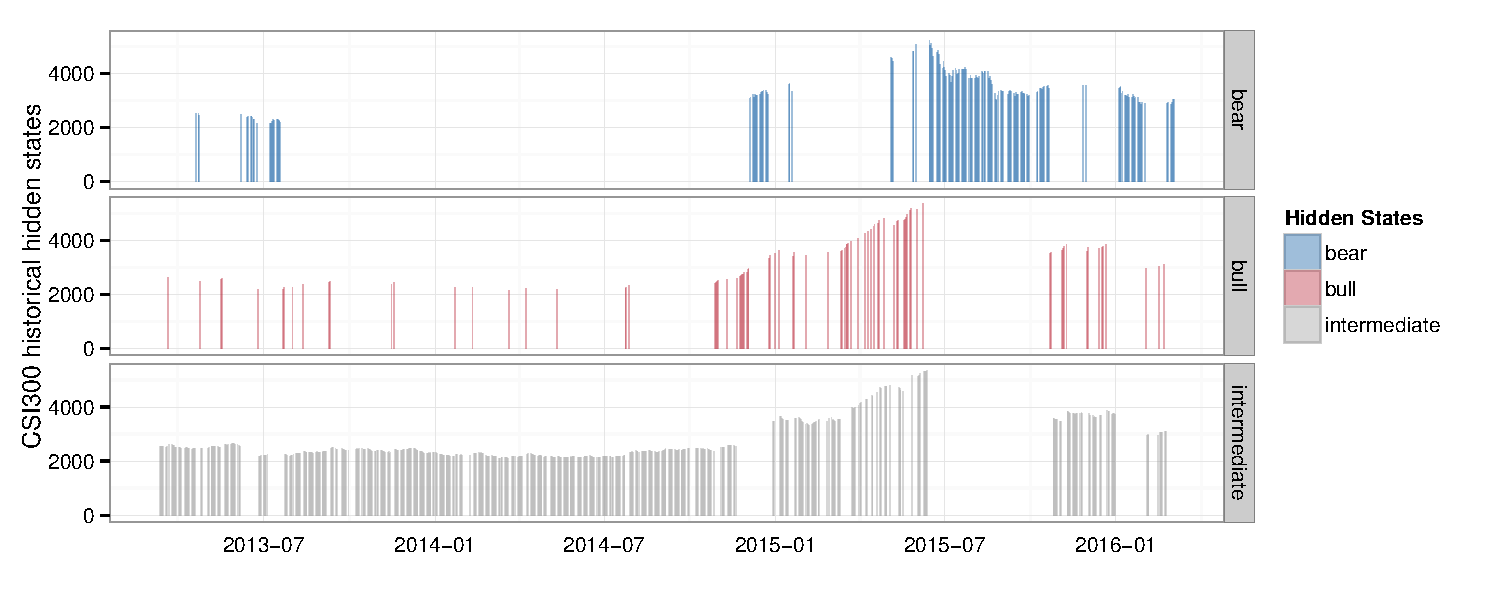
\includegraphics[width=0.49\textwidth]{daily/statesFig2.pdf}}
        \subfigure[Comparison between K-Means states and HMM hidden states]
            {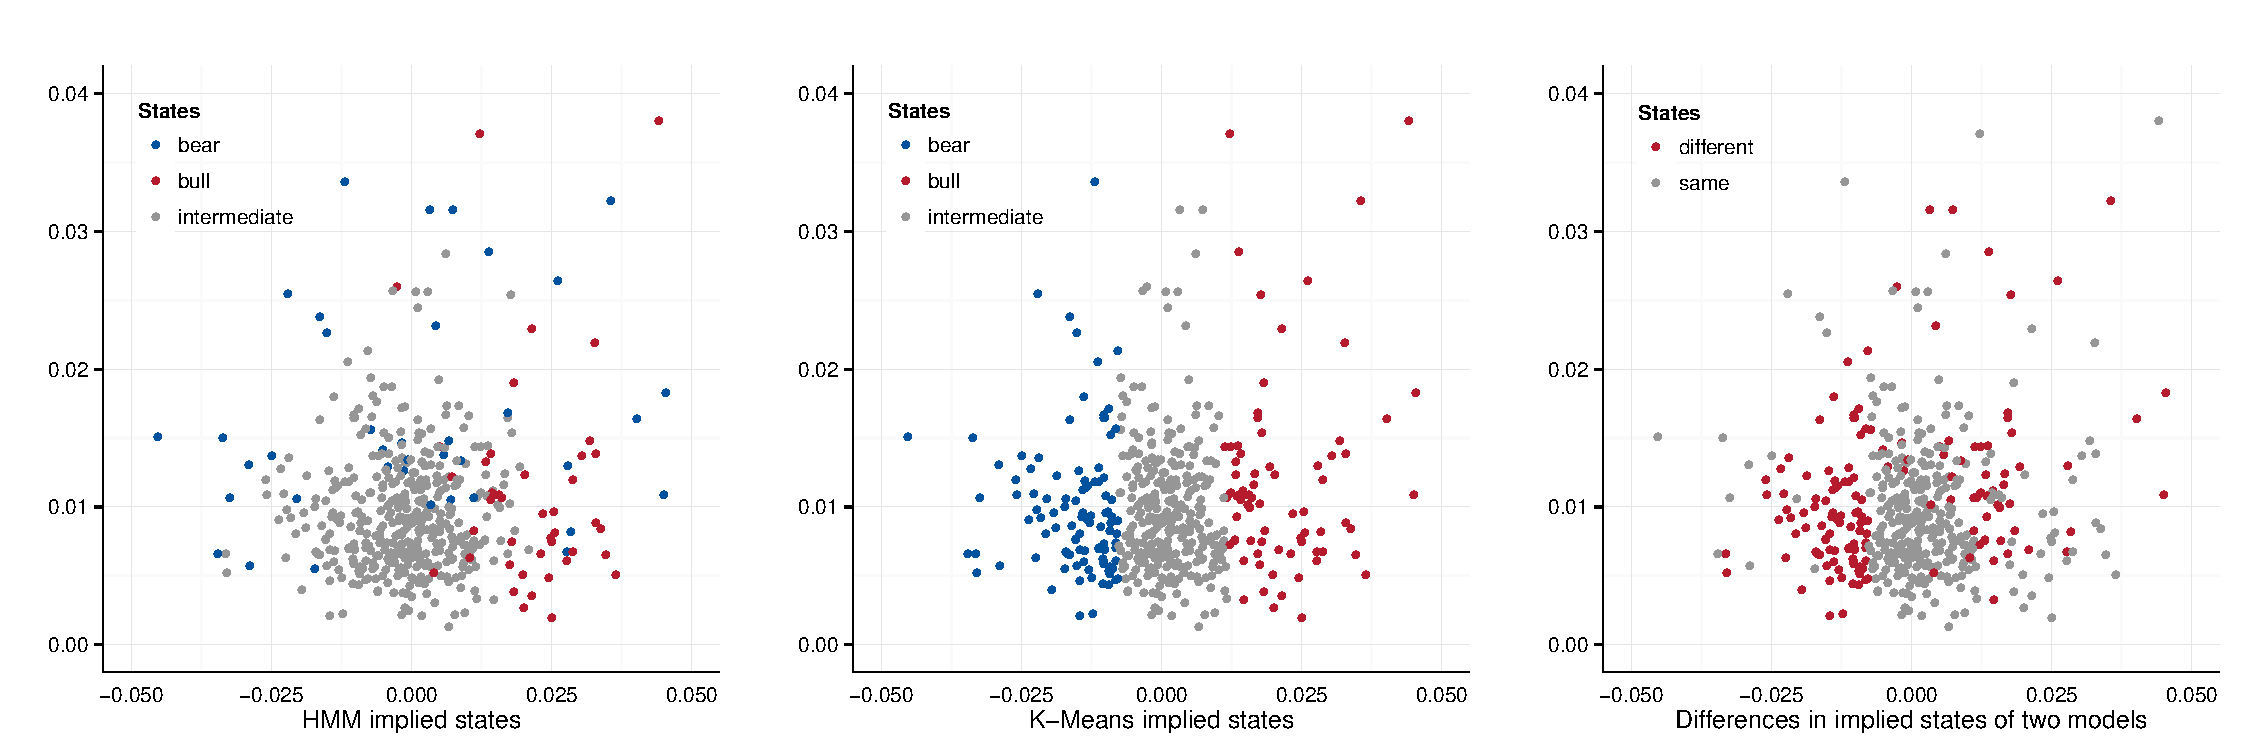
\includegraphics[width=0.49\textwidth]{daily/statesFig3.pdf}}
        \caption{CSI 300 daily data global decoding results}
        \label{fig:app:daily:states}
        \end{figure}

        \begin{figure}[!hbt]
        \center
        \subfigure[CSI 300 simulated prediction result out-of-sample part]
            {\includegraphics[width=0.49\textwidth]{daily/predictionFig2.pdf}}
        \subfigure[CSI 300 adaptive prediction]
            {\includegraphics[width=0.49\textwidth]{daily/predictionFig4.pdf}}
        \subfigure[CSI 300 simulated prediction result with confidence band]
            {\includegraphics[width=0.49\textwidth]{daily/predictionFig3.pdf}}
        \subfigure[CSI 300 adaptive prediction with confidence band]
            {\includegraphics[width=0.49\textwidth]{daily/predictionFig5.pdf}}
        \caption{CSI 300 daily data simulated prediction results}
        \label{fig:app:daily:prediction}
        \end{figure}


\section{CSI 300 60min return series}
\label{sec:fig:CSI:60}

\subsection{2013 - 2014}
\label{sec:fig:CSI:60:1314}

        \begin{figure}[!hbt]
        \center
        \subfigure[CSI 300 historical hidden states]
            {\includegraphics[width=0.49\textwidth]{60min_1314/statesFig2.pdf}}
        \subfigure[Comparison between K-Means states and HMM hidden states]
            {\includegraphics[width=0.49\textwidth]{60min_1314/statesFig3.pdf}}
        \caption{CSI 300 60min data global decoding results - 2013$\sim$2014}
        \label{fig:app:60:1314:states}
        \end{figure}

        \begin{figure}[!hbt]
        \center
        \subfigure[CSI 300 simulated prediction result out-of-sample part]
            {\includegraphics[width=0.49\textwidth]{60min_1314/predictionFig2.pdf}}
        \subfigure[CSI 300 adaptive prediction]
            {\includegraphics[width=0.49\textwidth]{60min_1314/predictionFig4.pdf}}
        \subfigure[CSI 300 simulated prediction result with confidence band]
            {\includegraphics[width=0.49\textwidth]{60min_1314/predictionFig3.pdf}}
        \subfigure[CSI 300 adaptive prediction with confidence band]
            {\includegraphics[width=0.49\textwidth]{60min_1314/predictionFig5.pdf}}
        \caption{CSI 300 60min data simulated prediction results - 2013$\sim$2014}
        \label{fig:app:60:1314:prediction}
        \end{figure}

\newpage
\subsection{2014 - 2015}
\label{sec:fig:CSI:60:1415}

        \begin{figure}[!hbt]
        \center
        \subfigure[CSI 300 historical hidden states]
            {\includegraphics[width=0.49\textwidth]{60min_1415/statesFig2.pdf}}
        \subfigure[Comparison between K-Means states and HMM hidden states]
            {\includegraphics[width=0.49\textwidth]{60min_1415/statesFig3.pdf}}
        \caption{CSI 300 60min data global decoding results - 2014$\sim$2015}
        \label{fig:app:60:1415:states}
        \end{figure}

        \begin{figure}[!hbt]
        \center
        \subfigure[CSI 300 simulated prediction result out-of-sample part]
            {\includegraphics[width=0.49\textwidth]{60min_1415/predictionFig2.pdf}}
        \subfigure[CSI 300 adaptive prediction]
            {\includegraphics[width=0.49\textwidth]{60min_1415/predictionFig4.pdf}}
        \subfigure[CSI 300 simulated prediction result with confidence band]
            {\includegraphics[width=0.49\textwidth]{60min_1415/predictionFig3.pdf}}
        \subfigure[CSI 300 adaptive prediction with confidence band]
            {\includegraphics[width=0.49\textwidth]{60min_1415/predictionFig5.pdf}}
        \caption{CSI 300 60min data simulated prediction results - 2014$\sim$2015}
        \label{fig:app:60:1415:prediction}
        \end{figure}

\newpage
\subsection{2015 - 2016}
\label{sec:fig:CSI:60:1516}

        \begin{figure}[!hbt]
        \center
        \subfigure[CSI 300 historical hidden states]
            {\includegraphics[width=0.49\textwidth]{60min_1516/statesFig2.pdf}}
        \subfigure[Comparison between K-Means states and HMM hidden states]
            {\includegraphics[width=0.49\textwidth]{60min_1516/statesFig3.pdf}}
        \caption{CSI 300 60min data global decoding results - 2015$\sim$2016}
        \label{fig:app:60:1516:states}
        \end{figure}

        \begin{figure}[!hbt]
        \center
        \subfigure[CSI 300 simulated prediction result out-of-sample part]
            {\includegraphics[width=0.49\textwidth]{60min_1516/predictionFig2.pdf}}
        \subfigure[CSI 300 adaptive prediction]
            {\includegraphics[width=0.49\textwidth]{60min_1516/predictionFig4.pdf}}
        \subfigure[CSI 300 simulated prediction result with confidence band]
            {\includegraphics[width=0.49\textwidth]{60min_1516/predictionFig3.pdf}}
        \subfigure[CSI 300 adaptive prediction with confidence band]
            {\includegraphics[width=0.49\textwidth]{60min_1516/predictionFig5.pdf}}
        \caption{CSI 300 60min data simulated prediction results - 2015$\sim$2016}
        \label{fig:app:60:1516:prediction}
        \end{figure}


\newpage
\section{CSI 300 10min return series}
\label{sec:fig:CSI:10}

\subsection{2013 - 2014}
\label{sec:fig:CSI:10:1314}

        \begin{figure}[!hbt]
        \center
        \subfigure[CSI 300 historical hidden states]
            {\includegraphics[width=0.49\textwidth]{10min_1314/statesFig2.pdf}}
        \subfigure[Comparison between K-Means states and HMM hidden states]
            {\includegraphics[width=0.49\textwidth]{10min_1314/statesFig3.pdf}}
        \caption{CSI 300 10min data global decoding results - 2013$\sim$2014}
        \label{fig:app:10:1314:states}
        \end{figure}

        \begin{figure}[!hbt]
        \center
        \subfigure[CSI 300 simulated prediction result out-of-sample part]
            {\includegraphics[width=0.49\textwidth]{10min_1314/predictionFig2.pdf}}
        \subfigure[CSI 300 adaptive prediction]
            {\includegraphics[width=0.49\textwidth]{10min_1314/predictionFig4.pdf}}
        \subfigure[CSI 300 simulated prediction result with confidence band]
            {\includegraphics[width=0.49\textwidth]{10min_1314/predictionFig3.pdf}}
        \subfigure[CSI 300 adaptive prediction with confidence band]
            {\includegraphics[width=0.49\textwidth]{10min_1314/predictionFig5.pdf}}
        \caption{CSI 300 10min data simulated prediction results - 2013$\sim$2014}
        \label{fig:app:10:1314:prediction}
        \end{figure}

\newpage
\subsection{2014 - 2015}
\label{sec:fig:CSI:10:1415}

        \begin{figure}[!hbt]
        \center
        \subfigure[CSI 300 historical hidden states]
            {\includegraphics[width=0.49\textwidth]{10min_1415/statesFig2.pdf}}
        \subfigure[Comparison between K-Means states and HMM hidden states]
            {\includegraphics[width=0.49\textwidth]{10min_1415/statesFig3.pdf}}
        \caption{CSI 300 10min data global decoding results - 2014$\sim$2015}
        \label{fig:app:10:1415:states}
        \end{figure}

        \begin{figure}[!hbt]
        \center
        \subfigure[CSI 300 simulated prediction result out-of-sample part]
            {\includegraphics[width=0.49\textwidth]{10min_1415/predictionFig2.pdf}}
        \subfigure[CSI 300 adaptive prediction]
            {\includegraphics[width=0.49\textwidth]{10min_1415/predictionFig4.pdf}}
        \subfigure[CSI 300 simulated prediction result with confidence band]
            {\includegraphics[width=0.49\textwidth]{10min_1415/predictionFig3.pdf}}
        \subfigure[CSI 300 adaptive prediction with confidence band]
            {\includegraphics[width=0.49\textwidth]{10min_1415/predictionFig5.pdf}}
        \caption{CSI 300 10min data simulated prediction results - 2014$\sim$2015}
        \label{fig:app:10:1415:prediction}
        \end{figure}

\newpage
\subsection{2015 - 2016}
\label{sec:fig:CSI:10:1516}

        \begin{figure}[!hbt]
        \center
        \subfigure[CSI 300 historical hidden states]
            {\includegraphics[width=0.49\textwidth]{10min_1516/statesFig2.pdf}}
        \subfigure[Comparison between K-Means states and HMM hidden states]
            {\includegraphics[width=0.49\textwidth]{10min_1516/statesFig3.pdf}}
        \caption{CSI 300 10min data global decoding results - 2015$\sim$2016}
        \label{fig:app:10:1516:states}
        \end{figure}

        \begin{figure}[!hbt]
        \center
        \subfigure[CSI 300 simulated prediction result out-of-sample part]
            {\includegraphics[width=0.49\textwidth]{10min_1516/predictionFig2.pdf}}
        \subfigure[CSI 300 adaptive prediction]
            {\includegraphics[width=0.49\textwidth]{10min_1516/predictionFig4.pdf}}
        \subfigure[CSI 300 simulated prediction result with confidence band]
            {\includegraphics[width=0.49\textwidth]{10min_1516/predictionFig3.pdf}}
        \subfigure[CSI 300 adaptive prediction with confidence band]
            {\includegraphics[width=0.49\textwidth]{10min_1516/predictionFig5.pdf}}
        \caption{CSI 300 10min data simulated prediction results - 2015$\sim$2016}
        \label{fig:app:10:1516:prediction}
        \end{figure}

% !TEX encoding = UTF-8 Unicode
\chapter{Model Realization Python Codes}
\label{app:code}

%%%%%%%%%%%%%%%%%%%%%%%%%%

\section{User manuscript}
\label{sec:code:manuscript}
All Python source codes for model realization are included in this appendix.
In this section we provide a brief instruction to these code files,
including the functionalities and how to run the codes,
after slight changes on file paths if needed.

Sec.\,\ref{sec:code:main} (\texttt{hmmMain.py}) is the main part of the model realization part,
which strictly follows the system we describe in Ch.\,\ref{chap:system}.
Sec.\,\ref{sec:code:class} (\texttt{hmmClass.py}) defines the Python class \texttt{HMM},
which is an encapsulated class object for the hidden Markov model.
Data members and member functions related to the model estimation are created within
(e.g.\,the observations, transition matrix, conditional distribution parameters, etc.).
One can find detailed information about the object in the introduction part of \texttt{hmmClass.py}.

Before running the \texttt{hmmMain.py} program,
make sure that \texttt{hmmClass.py} is under the same path of the main program.
In order to change the paths for data loading and results saving,
the user can modify the paths wherever \texttt{.from\_csv} and \texttt{.to\_csv} occur
and make the adjustments.
After certain changes, 
one can directly run \texttt{hmmMain.py} in an appropriate Python IDE.

Sec.\,\ref{sec:code:states} (\texttt{hmmStates.py}) is independent from the main program
and also requires (imports) the class definition module.
The program is intended to estimate the goodness of fitness of different models
with diverse number of hidden states,
which generates the results presented in Sec.\,\ref{sec:positive:result:states}.

%%%%%%%%%%%%%%%%%%%%%%%%%%

\newpage
\begin{spacing}{1.2}
\section{hmmMain.py}
\label{sec:code:main}
\begin{lstlisting}
# # # Graduation Thesis - Main
#
# The project is intended to construct a complete system for stock returns
# series prediction based on Hidden Markov Model. This program is the main 
# part of the project, realizing all aims of the empirical analysis part 
# along with other source code files.
#
# Source file lists
#   - hmmMain.py  : main part of the program
#   - hmmClass.py : include construction of the model, in the form of class
#   - hmmStates.py: a separate program to find the optimal number of hidden
#                   states
#
# Data files are import from .csv files and results will be stored in .csv
# format as well. Visualization analysis and presentation of the data will
# be realized in other programs.
 
# # # # # Program Starts Here # # # # #

## Library Import
import numpy as np
import pandas as pd
from math import sqrt
from sklearn.cluster import KMeans
from hmmClass import HMM

## Data Loading
dataYear = ''
dataFreq = 'daily'
dataFreqMin = 240
#dataFile = '/SP500Data_' + dataFreq + dataYear + '.csv'
dataFile = '/CSI300Data_' + dataFreq + dataYear + '.csv'
dataRaw = pd.DataFrame.from_csv(dataFreq + dataFile,index_col = False)
dataRet = pd.DataFrame({'ret': np.diff(np.log(dataRaw['close'])),
                        'time': dataRaw['time'][1:]})
                        
## In-sample & Out-of-sample Definition
numMin = 240 / dataFreqMin
numDay = len(dataRaw) / numMin
numStdDay = 5
lenInSample = int((numDay - numStdDay)*2/3)
lenOutSample = numDay - lenInSample - numStdDay
dataRetIn = dataRet.ix[0:(lenInSample + numStdDay)*numMin-1].copy()
dataRetIn.ix[:,'std'] = 0.0
for k in range(numStdDay*numMin,(lenInSample + numStdDay)*numMin):
    dataRetIn.ix[k,'std'] = np.std(dataRetIn.ix[(k-numStdDay*numMin):(k-1),
                                                'ret'])
dataRetIn = dataRetIn.tail(lenInSample*numMin)

## K-Means Clustering
# K-Means is used to find the initial probability distribution of the three
# states and corresponding conditional distribution parameters. 
# The parameters are used for HMM initialization.
numState = 3
label = ['bear','intermediate','bull']
modelKMeans = KMeans(n_clusters = numState).fit(dataRetIn[['ret','std']])
order = np.argsort(modelKMeans.cluster_centers_.T[0,:])
matParam = modelKMeans.cluster_centers_.T[:,order]
dataRetIn['label'] = ''
for k in range(0,len(dataRetIn)):
    dataRetIn.ix[dataRetIn.index[k],'label'] = label[np.where(order == modelKMeans.labels_[k])[0]]
matInit = np.array((dataRetIn['label'].value_counts())[label]/\
          len(dataRetIn))
matTrans = np.ones([numState,numState])/numState
dataRetIn.to_csv(dataFreq + '/dataReturnInSample' + dataYear + '.csv',
    index = False,encoding='utf-8',columns=['time','ret','std','label'])
dataRetIn.to_csv(dataFreq + '/dataPredict' + dataYear + '.csv',
    index = False,encoding='utf-8',columns=['time','ret','std'])

## Entire Period Estimation
dataRet = dataRet.ix[numStdDay*numMin:,]
model = HMM(dataRet,matTrans,matParam,matInit)
model.EM()
model.viterbi()
dataRet['label'] = ''
for k in range(0,len(dataRet)):
    dataRet.ix[dataRet.index[k],'label'] = label[int(model.matState[k])]
dataRet.to_csv(dataFreq + '/dataHistory' + dataYear + '.csv',
    index = False,encoding = 'utf-8',columns = ['time','ret','label'])

## Initialization
dataPredict = pd.DataFrame({'time':dataRet['time'],'ret':0.0,'std':0.0},
                            index = dataRet.index)
seqTrans = pd.DataFrame({'x11':0.0,'x12':0.0,'x13':0.0,
                         'x21':0.0,'x22':0.0,'x23':0.0,
                         'x31':0.0,'x32':0.0,'x33':0.0},
                         index = dataRet.index)
seqParam = pd.DataFrame({'mu1':0.0,'mu2':0.0,'mu3':0.0,
                         'sigma1':0.0,'sigma2':0.0,'sigma3':0.0},
                         index = dataRet.index)
seqParam.ix[(lenInSample+numStdDay)*numMin-1,] = \
    matParam.reshape(1,2*numState)
                         
## Estimation & Prediction
print 'HMM Loop starts now!'
for k in range(0,lenOutSample*numMin):
    print dataRet.ix[(lenInSample+numStdDay)*numMin+k,'time']
    model = HMM(dataRet.ix[:(lenInSample+numStdDay)*numMin+k-1],
                matTrans,matParam,matInit)
    model.EM()
    seqTrans.ix[(lenInSample+numStdDay)*numMin+k,] = model.matTrans.reshape(1,model.numState**2)
    seqParam.ix[(lenInSample+numStdDay)*numMin+k,] = model.matParam.reshape(1,2*model.numState)
    dataPredict.ix[(lenInSample+numStdDay)*numMin+k,'ret'] = model.matEnd.dot(model.matTrans).dot(model.matParam[0,])
    dataPredict.ix[(lenInSample+numStdDay)*numMin+k,'std'] = sqrt(((model.matEnd.dot(model.matTrans))**2).dot(model.matParam[1,]**2))
    pd.DataFrame(dataPredict.ix[(lenInSample+numStdDay)*numMin+k]).T.\
        to_csv(dataFreq + '/dataPredict' + dataYear + '.csv',mode = 'a',
        index = False,encoding = 'utf-8',
        header = False,columns = ['time','ret','std'])

seqTrans['time'] = dataRet['time']
seqParam['time'] = dataRet['time']
seqTrans.to_csv(dataFreq + '/matTrans' + dataYear + '.csv',
                index = False,encoding = 'utf-8',
                columns = ['time','x11','x12','x13',
                                  'x21','x22','x23',
                                  'x31','x32','x33'])
seqParam.to_csv(dataFreq + '/matParam' + dataYear + '.csv',
                index = False,encoding = 'utf-8',
                columns = list(['time']) + list(np.core.defchararray.add(list(np.repeat('mu',3)),map(str,range(1,4)))) \
                + list(np.core.defchararray.add(list(np.repeat('sigma',3)),map(str,range(1,4)))))
\end{lstlisting}
\newpage

\section{hmmClass.py}
\label{sec:code:class}
\begin{lstlisting}
# # # Graduation Thesis - HMM Class Definition
#
# This program include the construction of a HMM class. The members are 
# listed as follows:
#
# Member Data:
#   - obs: the observed sequence/time series
#   - numState: the number of hidden states
#   - matInit: the original probability distribution of hidden states
#   - matTrans: the state transition probability matrix
#   - matParam: the conditional distribution parameters of the observed 
#               sequence, corresponding to each hidden state
#   - matDist: the probability distribution matrix, corresponding to each 
#              observation at each state
#   - matEnd: the probability distribution of hidden states at the last 
#             observation
#
# Member Functions:
#   - __init__: built-in initialization function of the class
#   - forward: calculates the forward probability of observed sequence
#   - backward: calculates the backward probability of observed sequence
#   - expState: calculates the expectation of states
#   - expStateTrans: calculates the expected state transition probability
#   - EM: the major part of HMM parameter (including state transition 
#         probabilities, conditional distribution parameter, initial and 
#         final state distribution) estimation using Baum-Welch algorithm
#   - viterbi: global decoding to find the most probable sequence of 
#              hidden states using Viterbi algorithm

# # # # # Program Starts Here # # # # #
import numpy as np
import pandas as pd
from matplotlib.mlab import *

class HMM:
    def __init__(self,seqObserv,matTrans,matParam,matInit):
        '''HMM is the class defined to hold necessary data and functions 
        for a standard hidden Markov model. The initialization of a HMM 
        class requires 4 inputs given in the parameter list.
        
        Parameters
        ----------
        seqObserv : a data frame holding the stock return series
        matTrans : the initial state transition probability matrix
        matParam : the initial conditional distribution parameters 
                   corresponding to each hidden state
        matInit : the initial probability distribution of hidden states'''
        self.obs = seqObserv['ret'].copy()
        self.matTrans = matTrans.copy()
        self.matInit = matInit.copy()
        self.numState = matTrans.shape[0]
        self.matParam = matParam.copy()
        self.matDist = np.zeros([self.matTrans.shape[0],len(self.obs)])
        matDistTemp = pd.DataFrame(index = self.obs.index)
        for k in range(0,self.matTrans.shape[0]):
            matDistTemp['x' + str(k)] = normpdf(self.obs,self.matParam[0,k],self.matParam[1,k])
        self.matDist = np.array(matDistTemp.T)
    
    def forward(self):
        T = len(self.obs)
        alpha = np.zeros([self.numState,T])
        scale = np.zeros(T)
        alpha[:,0] = self.matInit[:] * self.matDist[:,0]
        scale[0] = np.sum(alpha[:,0])
        alpha[:,0] /= scale[0]
        for t in range(1,T):
            if np.sum(self.matDist[:,t]) != 0:
                alpha[:,t] = np.dot(alpha[:,t-1].T,self.matTrans).T *\
                             self.matDist[:,t]
                scale[t] = np.sum(alpha[:,t])
                alpha[:,t] /= scale[t]
            else:
                alpha[:,t] = alpha[:,t-1]
                scale[t] = scale[t-1] 
        logp = np.sum(np.log(scale[:]))
        return alpha, scale, logp
        
    def backward(self,scale):
        T = len(self.obs)
        beta = np.zeros([self.numState,T])
        beta[:,T-1] = 1/scale[T-1]
        for t in range(T-1,0,-1):
            beta[:,t-1] = np.dot(self.matTrans,
                                 (self.matDist[:,t]*beta[:,t]))
            beta[:,t-1] /= scale[t-1]
        return beta
        
    def expState(self,alpha,beta):
        gamma = np.zeros(alpha.shape)
        gamma = alpha[:,:] * beta[:,:]
        gamma = gamma / ((np.sum(gamma,0) == 0) + np.sum(gamma,0))
        return gamma
        
    def expStateTrans(self,alpha,beta):
        T = len(self.obs)
        xi = np.zeros((self.numState,self.numState,T-1))   
        for t in range(T-1):
            denom = np.dot(np.dot(alpha[:,t].T, self.matTrans) * \
                    self.matDist[:,t+1].T,beta[:,t+1])
            for i in range(self.numState):
                numer = alpha[i,t] * self.matTrans[i,:] * \
                        self.matDist[:,t+1].T * beta[:,t+1].T
                xi[i,:,t] = numer / (denom + (denom == 0))
        return xi
        
    def EM(self):
        T = len(self.obs)
        criterion = 0.001
        alpha, scale, logp = self.forward()
        beta = self.backward(scale)            
        gamma = self.expState(alpha,beta)    
        xi = self.expStateTrans(alpha,beta)
        matDistTemp = self.matDist
        loop = 0
        while True:
            for i in range(0,self.numState):
                denominator = np.sum(gamma[i,0:T-1])
                for j in range(0,self.numState): 
                    numerator = np.sum(xi[i,j,0:T-1])
                    self.matTrans[i,j] = numerator / \
                                    (denominator + (denominator == 0))
            
            tempMu = np.array([np.sum(gamma*np.array(self.obs.T),1)/np.sum(gamma,1)])
            tempSigma = np.sqrt(np.array([np.sum(gamma*(np.array(self.obs.T) - tempMu.T)**2,1) / np.sum(gamma,1)]))
            self.matParam[0,:] = tempMu
            self.matParam[1,:] = tempSigma
            matDistTemp = pd.DataFrame(index = self.obs.index)
            for k in range(0,self.matTrans.shape[0]):
                matDistTemp['x' + str(k)] = normpdf(self.obs,self.matParam[0,k],self.matParam[1,k])
            matDistTemp = np.array(matDistTemp.T)
            
            self.matDist = matDistTemp
            self.matInit = gamma[:,0]
            self.matEnd = gamma[:,-1]
            
            alpha, scale, logpNew = self.forward()
            beta = self.backward(scale)            
            gamma = self.expState(alpha,beta)    
            xi = self.expStateTrans(alpha,beta)
            
            delta = abs(logpNew - logp)
            logp = logpNew
            loop += 1
            if delta <= criterion:
                break
        
        self.valAIC = -2*logp + 2*(self.numState**2 + 2*self.numState - 1)
        self.valBIC = -2*logp + \
                      np.log(T)*(self.numState**2 + 2*self.numState - 1)
                
    def viterbi(self):
        T = len(self.obs)
        psi = np.zeros([self.numState,T])
        delta = np.zeros([self.numState,T])
        matState = np.zeros(T)
        temp = np.zeros([self.numState,self.numState])

        delta[:,0] = np.log(self.matInit) + np.log(self.matDist[:,0])
        for t in range(1,T):
            temp = (delta[:,t-1] + np.log(self.matTrans.T)).T
            ind = np.argmax(temp, axis = 0)
            psi[:,t] = ind
            delta[:,t] = np.log(self.matDist[:,t]) + \
                         temp[ind,range(self.numState)]
        
        max_ind = np.argmax(delta[:,T-1])
        matState[T-1] = max_ind
        for t in reversed(range(0,T-1)):
            matState[t] = psi[matState[t+1],t+1] 
        
        self.logProbState = delta[:,T-1][max_ind]
        self.matState = matState    
\end{lstlisting}
\newpage

\section{hmmStates.py}
\label{sec:code:states}
\begin{lstlisting}
# # # Graduation Thesis - Number of States 
#
# This program is very similar to the main one, except that is elminates 
# the part of prediction and focuses on evaluating the goodness of fit of 
# models with different number of hidden states. Notice that the analysis 
# is performed only for CSI300 daily data.
#
# Data files are import from .csv files and results will be stored in .csv
# format as well.
 
# # # # # Program Starts Here # # # # #

## Library Import
import numpy as np
import pandas as pd
from sklearn.cluster import KMeans
from hmmClass import HMM

## Data Loading
dataPath = 'states'
dataPathMin = 240
dataRaw = pd.DataFrame.from_csv('daily/CSI300Data_daily.csv',
                                index_col = False)
dataRet = pd.DataFrame({'ret': np.diff(np.log(dataRaw['close'])),
                        'time': dataRaw['time'][1:]})
                        
## In-sample & Out-of-sample Definition
numMin = 240 / dataPathMin
numDay = len(dataRaw) / numMin
numStdDay = 5
lenInSample = int((numDay - numStdDay)*2/3)
lenOutSample = numDay - lenInSample - numStdDay
dataRetIn = dataRet.ix[0:(lenInSample + numStdDay)*numMin-1].copy()
dataRetIn.ix[:,'std'] = 0.0
for k in range(numStdDay*numMin,(lenInSample + numStdDay)*numMin):
    dataRetIn.ix[k,'std'] = np.std(dataRetIn.ix[(k-numStdDay*numMin):(k-1),
                                                'ret'])
dataRetIn = dataRetIn.tail(lenInSample*numMin)

## Loop for Different Number of States
seqAIC = pd.DataFrame({'number':range(2,7),'value':0},index = range(2,7))
seqBIC = pd.DataFrame({'number':range(2,7),'value':0},index = range(2,7))

for numState in range(2,7):
    print 'Number of States:', numState
    ## K-Means Clustering
    label = range(0,numState)
    modelKMeans = KMeans(n_clusters = numState).\
                         fit(dataRetIn[['ret','std']])
    order = np.argsort(modelKMeans.cluster_centers_.T[0,:])
    matParam = modelKMeans.cluster_centers_.T[:,order]
    dataRetIn['label'] = ''
    for k in range(0,len(dataRetIn)):
        dataRetIn.ix[dataRetIn.index[k],'label'] = label[np.where(order == modelKMeans.labels_[k])[0]]
    matInit = np.array((dataRetIn['label'].value_counts())[label]/\
            len(dataRetIn))
    matTrans = np.ones([numState,numState])/numState
    
    ## Entire Period Estimation
    dataRet = dataRet.ix[numStdDay*numMin:,]
    model = HMM(dataRet,matTrans,matParam,matInit)
    model.EM()
    seqAIC.ix[numState,'value'] = model.valAIC
    seqBIC.ix[numState,'value'] = model.valBIC
    
seqAIC.to_csv(dataPath + '/aic.csv',index = False,encoding = 'utf-8')
seqBIC.to_csv(dataPath + '/bic.csv',index = False,encoding = 'utf-8')
\end{lstlisting}
\end{spacing}

%%%%%%%%%%%%%%%%%%%%%%%%%%

\backmatter

\begin{spacing}{1.1}
\bibliography{ref/ref}
\end{spacing}

%%==================================================
%% thanks.tex for SJTU Bachelor Thesis
%% version: 0.5.2
%% Encoding: UTF-8
%%==================================================

\begin{thanks}

I would like to express my great gratitude to my parents, teachers and friends.
Thank you for backing me up all the time.
It is never tough to come up with an undergraduation thesis,
but it is never easy to keep fighting until the last second of my college life even I am graduating.
Life has been especially hard in the last year,
and thanks to you all because I know I would be confused without your advice and encouragements.

Thanks to Prof. Jianzhong Lin for being the my supervisor of the thesis, 
and for spending time reading the thesis and providing suggestions.

Thanks to my parents for never pushing me even slightly.
Thank you for telling me to stop and take a break whenever I am working hard.
I know I would never stop, 
yet I still need this to find solace when I am too frustrated to rest.

Special thanks to Prof. Jinglai Li for introducing me to the realm of academic research,
and for all the supports during my graduate school applications.
Special thanks to Qun Zhao, 
a true friend and a great mentor,
for all kinds of advice and help on career path and academic research and 
other things that are too numerous to mention.
Special thanks to my competitors during all exams, interviews and contests.
Thank you for always reminding me that there is still a long long way to go,
to become a better person and to do more things.

Finally, special thanks to myself,
for never giving up and never having the thought to give up,
for all the fun and excitement during the life adventure,
and for all the passion that keeps me fighting and looking for new funs.

Life sucks when you are ordinary.
So be more than that,
beat whatever stands between yourself and your goals,
especially your past selves,
the vulnerable and weak ones that hinder you from going further.
If you should fail, you fail,
but never stop trying.
If you would live, you live,
and always live better, 
long and prosper.

% Special thanks to my future girlfriend, 
% if there should be one,
% for not showing up during the last year so that I could be fully concentrated on whatever I was doing.
% Now it is time to show yourself.
% 
% Special and great thanks to Fat Huang, Big Huang, Small Huang, 
% Small Hua, Small Hui, Small Bai, Small Hei, et al., 
% from PYG Library, without whom I would never have enjoyed the last year so much.
%
% Life sucks when you are ordinary.
% Fuck life, and enjoy it.

\end{thanks}



% 发表文章目录
%\include{body/pub}
% 参与项目列表
%\include{body/projects}

%%%==================================================
%% bigabstract.tex for SJTU Bachelor Thesis
%% version: 0.5.2
%% Encoding: UTF-8
%%==================================================

\begin{bigabstract}

In the area of quantitative finance,
research and analysis on stock return series is one of the most concentrated topics 
shared by both the industry and the academia.
Conditional on different market states,
the distributions of stock returns vary largely,
and the hidden Markov model is able to quantitatively depict the state-dependency of stock returns.

This thesis is intended to implement the hidden Markov model to 
analyze and describe the hidden states of stock markets,
from which to deduce the conditional distributions of the returns,
and carry out stock return series prediction based on the model.

In this thesis, 
we provide analyses and explanations with details on the model.
Formal definition and formulation of a hidden Markov is provided,
followed by the derivation of marginal distributions and other primary statistics.
We introduce the forward and backward procedure and 
expectation maximization algorithm for model parameters estimation,
after which forecast distributions are also covered.
In order to excavate information about the historical hidden states,
the concepts of state probabilities, local decoding and global decoding are introduced,
and we use the Viterbi algorithm to conduct global decoding for the hidden Markov model.

Based on this theoretical model and some other related knowledge and techniques,
we construct a complete stock return series prediction system.
We achieve the aim of prediction through three steps,
model initialization with K-Means clustering,
model estimation with expectation maximization algorithm,
and iterative one-step forecasts for the out-of-sample data.
The task of model realization is accomplished through Python programming.

We then use the realized system to perform empirical analysis and model validation 
on the CSI 300 Index from Chinese stock market and the S\&P 500 Index from the U.S. stock market.
After making appropriate assumptions and conjectures,
we in order analyze the S\&P 500 daily return data, CSI 300 daily data,
and CSI 300 medium frequency (60min and 10min) data.
Thorough analyses and comparions are carried out and numerical results are provided,
along with presentations of results visualization.

Additionally, we provide further discussions on unaddressed issues remained 
in the model construction part and empirical analysis part,
including the time lag effect and model estimations for other more general hidden Markov models.
To ameliorate the time lag effect we propose two potential solutions,
which are adopting rolling windows for sample data censoring and 
a data reweighting algorithm named exponantially weighted expectation maximization.
For more general hidden Markov models,
we restate the problem formulation and provide the derivations of some key statistics.
The particle filter method is also introduced as a standard tool for model estimation.
We hope to solve these remaining problems and further our research on the model in future works.

\end{bigabstract}


%%%%%%%%%%%%%%%%%%%%%%%%%%
\end{document}